% use the MIT thesis document class
\documentclass[12pt]{mitthesis}

% some packages needed for library-compliant typesetting
\usepackage{lgrind}
\usepackage{cmap}
\usepackage[T1]{fontenc}
\pagestyle{plain}

% packages Scott put into the template
\usepackage{pdfpages} % to include pdfs
\usepackage{caption} % for caption*
\usepackage{graphicx} % for figures
\usepackage{chapterbib} % for bibliographies in each chapter
\usepackage{tocloft} % for fixing table of contents
\usepackage{booktabs} % for nice tables

% options for controlling the table of contents typesetting
\setcounter{tocdepth}{1} % only show chapters in table of contents
\renewcommand{\cftchapfont}{\rmfamily} % chapters in not bold
\renewcommand{\cftchappagefont}{\rmfamily} % page in not bold

% Packages Claire needed for individual papers
\usepackage[colorlinks=false]{hyperref} % for links and urls
\usepackage{amsmath,amssymb} % for math
\usepackage{color,soul} % for highlighting
\usepackage{rotating,multirow} % for nice tables
\usepackage[numbers]{natbib}
\usepackage[above]{placeins} % for FloatBarrier
\usepackage{amsmath} % for pretty fraction text
\usepackage{booktabs} % for multi-line tables
\usepackage{lineno} % for line numbers
\usepackage{geometry} % for supp fig large pages

\begin{document}

\title{Mining the human microbiome for clinical insight}

\author{Claire Marie Noëlle Duvallet}

\prevdegrees{B.S., Columbia University (2013)}

\department{Department of Biological Engineering}

\degree{Doctor of Philosophy in Biological Engineering}

% Valid degree months are September,
% February, or June.  The default is June.
\degreemonth{June}
\degreeyear{2019}
\thesisdate{11 January 2019}

%% By default, the thesis will be copyrighted to MIT.  If you need to copyright
%% the thesis to yourself, just specify the `vi' documentclass option.  If for
%% some reason you want to exactly specify the copyright notice text, you can
%% use the \copyrightnoticetext command.
%\copyrightnoticetext{\copyright IBM, 1990.  Do not open till Xmas.}

% If there is more than one supervisor, use the \supervisor command
% once for each.
\supervisor{Eric J. Alm}{Professor}

% This is the department committee chairman, not the thesis committee
% chairman.  You should replace this with your Department's Committee
% Chairman.
\chairman{Forest White}{Chair of Graduate Program, Department of Biological Engineering}

% Make the titlepage based on the above information.  If you need
% something special and can't use the standard form, you can specify
% the exact text of the titlepage yourself.  Put it in a titlepage
% environment and leave blank lines where you want vertical space.
% The spaces will be adjusted to fill the entire page.  The dotted
% lines for the signatures are made with the \signature command.
\maketitle

% The abstractpage environment sets up everything on the page except
% the text itself.  The title and other header material are put at the
% top of the page, and the supervisors are listed at the bottom.  A
% new page is begun both before and after.  Of course, an abstract may
% be more than one page itself.  If you need more control over the
% format of the page, you can use the abstract environment, which puts
% the word "Abstract" at the beginning and single spaces its text.

% You can either \input (*not* \include) your abstract file, or you can put
% the text of the abstract directly between the \begin{abstractpage} and
% \end{abstractpage} commands.
\cleardoublepage
\setcounter{savepage}{\thepage}
\begin{abstractpage}
%% The text of your abstract and nothing else (other than comments) goes here.
%% It will be single-spaced and the rest of the text that is supposed to go on
%% the abstract page will be generated by the abstractpage environment.

The human microbiome is essential for health and has been implicated in many diseases.
DNA sequencing has enabled the detailed characterization of these human-associated microbial communities, leading to a rapid expansion in studies investigating the human microbiome.
%However, extracting clinically-relevant associations from microbiome datasets remains challenging because of the high dimensional nature of the data and variability across studies.
In this thesis, I describe three projects which overcome various data analysis challenges to extract useful clinical insights from microbiome data.
In the first project, I present an analysis of lung, stomach, and oropharyngeal microbiomes.
I leverage data collected from multiple sites per patient to identify aspiration-associated changes in the relationships between aerodigestive communities, discovering new properties of the aerodigestive microbiome and suggesting new approaches for treatment.
%These changes suggest new approaches for developing diagnostics and treatments for aspiration-related respiratory complications.
%I leverage data collected from multiple sites per patient to find aspiration-associated changes in the relationships between aerodigestive communities which suggests new targets for treatment and diagnosis.
In the second project, I perform a meta-analysis of case-control gut microbiome datasets with standard data processing and analysis methods.
I find consistent patterns characterizing disease-associated microbiome changes and a set of shared associations which could inform clinical treatment and therapeutic development approaches for many different microbiome-mediate diseases.
In the third project, I describe a framework for rational donor selection in fecal microbiota transplant clinical trials.
In this framework, knowledge derived from clinical and basic science research is used to inform which donor is selected for fecal transplants, increasing the likelihood of successful trials.
Together, these projects demonstrate a variety of approaches to mine the human microbiome for clinically-relevant insights and suggests multiple avenues forward for translating findings from microbiome data analyses into clinical impact.

\end{abstractpage}

\cleardoublepage

\section*{Acknowledgments}

Mentors:
Rafa - will always be a friend of the lab
Jim
Deb
Ilana - for being the mentor I didn't know I needed

Thomas - being my first introduction to computational work with patience and enthusiasm, enabling me to find my passion here
Mariana - drive and ability to make impossible things actually happen was an inspiration, expanded the scope of what a PhD student could do
Scott - being a role model, mentor, collaborator, and now close friend. Hope you remain all four forever. Also for encouraging me to start doing diversity and REFS
Sean Gibbons - modeling pure interest in science for the sake of science, encouraging me and being patient when I thought it was all fake, modeling success and being a joy to work with

Peers:
Nathaniel
Diversity co-conspirators: Scott and Manu, Bevin, and now my GSC crew for revitalizing me in the work (Nas, Josue, Danielle, German, Halston, and Bianca)

Funding:
NDSEG
Siebel

Friends, family, and frisbee
Carolyn and Megan
Andee and Shelby
Janyne for keeping me adventuring
sMITe
Felix (for GTD, 20% rule, and inspiration to version control everything)
ET (for putting us to shame by having a job and real life)
Parents (for supporting me, recognizing my passions better than I do, and listening to me talk about poop over many dinners)

\pagestyle{plain}
\include{contents}

% include each tex file
%% This is an example first chapter.  You should put chapter/appendix that you
%% write into a separate file, and add a line \include{yourfilename} to
%% main.tex, where `yourfilename.tex' is the name of the chapter/appendix file.
%% You can process specific files by typing their names in at the
%% \files=
%% prompt when you run the file main.tex through LaTeX.

\chapter{Introduction}

\section{The human microbiome in health and disease}

The microbes that live in and on our bodies make up the human microbiome, are essential for health, and have been implicated in many diseases.
Almost all human body sites are colonized by microbes, ranging from the gut, the largest human-associated microbial community, to the lungs, which were for many years considered sterile \cite{sender-2016-bhratio,beck-2012-lungmicrobiome}.
These microbial communities perform essential functions for health, including fighting off and preventing infections, regulating host metabolism and interacting with the immune system, and metabolizing xenobiotics or other compounds which are indigestible by the host.
Additionally, perturbations in human microbiomes have been implicated in many diseases, including inflammatory, metabolic, neurological, and respiratory conditions \cite{beck-2012-lungmicrobiome,ibd-papa,ridaura-2013-obfmt,hsiao-2013-autism}.

The potential for microbiome-based therapies to improve human health and address a broad range of diseases has led to a recent expansion of research and clinical studies in this field.
Much of the emerging research has been driven in part by the increasing accessibility of DNA sequencing technology, which can provide a detailed view of the bacteria in these communities without the need for time-consuming and difficult culturing experiments \cite{hmp-2012}.
However, identifying clinically-relevant associations from microbiome studies remains challenging \cite{knights-2011-predictivevalue}.
Microbiome datasets are high-dimensional, with hundreds to thousands of bacterial species measured in usually only tens to hundreds of patient samples.
Microbial communities are also highly variable across people, making it more difficult to identify individual bacterial biomarkers that can consistently distinguish health and disease across many different patients.
Finally, microbiome datasets provide a window into associations but not causal relationships, and researchers must perform follow-up mechanistic studies or clinical trials to confirm the clinical relevance of any identified associations.
In this thesis, I present unique analyses of microbiome data which overcome some of these challenges and which illustrate a variety of approaches for extracting useful clinical insights from mining microbiome data.
Together, the following chapters aim to move findings from the individual microbiome data analyses beyond statistical significance and toward clinical meaningfulness.

\section{Multi-site sampling to identify clinical associations in the aerodigestive microbiome}

In Chapter \ref{chap:aspiration}, I leverage simultaneous sampling within patients to identify clinically-relevant aerodigestive microbiome characteristics that distinguish patients with swallowing dysfunction from those with normal swallow.
The current gold standard to diagnose aspiration resulting from impaired swallow function involves imaging a patient as they ingest different quantities and consistencies of contrast material \cite{cook-1999-dysphagia}, but identifying lung microbial biomarkers could provide a useful non-radioactive alternative to this diagnosis.
Additionally, patients with impaired swallow function are at higher risk for respiratory infections, but the extent to which the lung microbiome is perturbed by aspiration and thus potentially involved in mediating this risk is unknown \cite{cook-1999-dysphagia,thomson-2016-asppneumo}.
Finally, clinical interventions to treat respiratory symptoms in patients with impaired swallow focus on preventing material transfer from the stomach into the lungs, for example via anti-reflux medication or fundoplication surgery \cite{goldin-2006-fundo,lee-2008-fundo}.
However, the clinical utility of these interventions in pediatric populations is not fully established, and the extent to which the gastric vs. mouth microbiome mediates respiratory complications is not known.

In this study, I analyzed a set of aerodigestive microbiome samples collected from over 200 patients at Boston Children's Hospital.
I first show that lung and stomach microbiomes are highly variable across people and driven primarily by person rather than body site, complicating the search for a reliable microbial biomarker of aspiration across patients.
I overcome this challenge by leveraging the fact that we have multiple samples per patient, comparing instead the within-patient \textit{relationships} between microbial communities in the aerodigestive tract of patients with and without aspiration.
Using this approach, I show that aspiration shifts lung microbial communities toward the oropharyngeal but not the stomach microbiome, suggesting that the mouth is likely an important source of lung microbiome changes in these patients.
Thus, approaches for treating aspiration-related respiratory symptoms should target microbial transfer from the mouth into the lungs in addition to focusing on the gastric-lung axis, as most current interventions do.
This study also illustrates the power of multi-site within-patient sampling to overcome variability across people to identify clinically meaningful microbiome-based biomarkers.

\section{Re-analyzing datasets to find consistent patterns of associations between the gut microbiome and disease}

In Chapter \ref{chap:meta-analysis}, I perform a meta-analysis of 28 case-control gut microbiome studies across 10 diseases to synthesize findings across studies and identify generalizable associations.
Although the human gut microbiome has been extensively studied in many diseases, there is little consensus on which disease associations are consistent across patient cohorts.
In other fields like medicine or psychology, consensus is usually achieved through meta-analyses of published literature \cite{glass-1976}.
However, comparing published results across microbiome studies is not straightforward.
The field lacks standard data processing and analysis methods, making many reported results impossible or inappropriate to compare directly between studies.
For example, different studies often use incompatible bioinformatics or statistical methods: they may compare bacteria at different taxonomic levels and use different bioinformatics workflows, and they may identify significant associations through univariate statistical tests or machine learning models, results from which can not be readily compared \cite{edd-singh,crc-baxter,crc-zeller,ob-zupancic}.
Additionally, studies led by clinicians often ask very different questions of the data than studies led by microbial ecologists, and so the reported results are not necessarily representative of the comprehensive information contained in the full dataset \cite{asd-son,ra-scher,nash-wong}.
This issue is especially relevant in this field, where non-invasive sample collection and open-source bioinformatics software suites have made microbiome research accessible to a broad range of scientists and clinicians.

In this chapter, I perform a meta-analysis of gut microbiome studies which overcomes many of these challenges by reprocessing and reanalyzing raw data with standard methods.
Even though specific bacterial associations vary across studies of the same disease, I identify patterns of general microbiome shifts which are consistent  and which suggest different approaches for developing microbiome-based therapeutics.
When looking across multiple diseases, I find a set of bacteria which are non-specifically associated with health and disease, perhaps forming a shared or core response to general health and disease status.
These results highlight the importance of contextualizing results from individual studies within the existing body of work, and also hints at the possibility of developing broadly beneficial targeted probiotic and antibiotic therapies.

\section{Enabling more powerful meta-analyses by developing a batch correction method for microbiome data}

Motivated and enabled by the work presented in Chapter \ref{chap:meta-analysis}, I present a method to correct for batch effects in case-control microbiome studies in Chapter \ref{chap:perc-norm}.
Traditionally, meta-analyses compile published p-values and effect sizes and determine their consistency, significance, and magnitude across studies to glean an overall understanding of true effects \cite{glass-1976}.
However, this is challenging to do in the microbiome research field for reasons described above and in Chapter \ref{chap:meta-analysis}.
A more powerful way to synthesize findings across studies is to combine the raw data and re-perform analyses on this expanded sample size.
However, analyzing raw data combined from multiple studies is not appropriate without first correcting for batch effects.
In microbiome data, batch effects result from biological and technical variation between studies and although statistical methods to correct for these have been developed for other `omics data types, few are applicable for microbiome data \cite{gibbons-2018}.

In this chapter, we describe a method to correct for batch effects in microbiome data.
Briefly, the method converts the abundances of taxa in case samples to percentiles of their respective distributions in the control samples within each study, in essence considering control samples as the null.
Assuming that control patients should represent biologically similar groups, this allows for pooling of percentile-normalized data across studies.
We show that this non-parametric method successfully removes batch effects in case-control studies, enabling more powerful analyses on combined microbiome data and reducing the number of false positives from individual analyses.
My main contributions to this joint work were processing the datasets used to develop and test the method and implementing the method into a popular microbiome software suite, QIIME 2 \cite{qiime2}, expanding its reach and accessibility.

\section{Translating microbiome research through rationally designed fecal microbiota transplant clinical trials}

In Chapter \ref{chap:donor-selection}, I present a framework for rationally selecting donors in fecal microbiota transplant (FMT) clinical trials.
In recurrent \textit{Clostridium difficile} infection (rCDI), FMTs have proven themselves as a remarkably effective clinical treatment, generating excitement about the clinical potential of FMTs in other diseases \cite{quraishi-2017-rcdifmt,bafeta-2017-fmt}.
Clinical trials in non-rCDI diseases can be used to identify promising conditions in which the microbiome may have a causal role to play.
However, although there is little donor-dependent variability in FMT efficacy in rCDI, it is becoming apparent that in many other non-rCDI conditions, donor heterogeneity likely plays a role in patient response \cite{moayyedi-2015,olesen-2018-superstool}.
Thus, as FMT trials expand to new indications, many trials may fail not because the indication was not amenable to improvement by FMT but rather because an ineffective donor was chosen.
As a consequence, excitement and support for FMT research will be dampened, slowing progress toward finding clinical applications of microbiome-based therapies.

In this chapter, we present an approach for selecting donors in FMT trials to increase the likelihood that these trials will succeed.
In our proposed framework, a clinician applies her existing knowledge and hypotheses for how her indication of interest is being mediated by the microbiome to drive the donor selection process.
We present four types of disease models to describe underlying processes mediating microbiome-related diseases: acute dysbiosis, mediation by individual taxa, missing or overactive community function, and complex host-microbiome interactions.
We suggest associated donor selection strategies for each of these disease models, and provide case studies illustrating the process of selecting donors rationally.
Finally, I perform a power simulation which finds that most FMT trials are unlikely to be powered enough to identify the key donor bacteria mediating patient responses to FMT.
Thus, to successfully make discoveries from completed trials, clinicians should perform hypothesis-driven retrospective analyses and plan for these during the clinical trial design process, for example by collecting paired donor and patient and/or longitudinal samples.
The framework that we present encourages clinicians to leverage their clinical experience, existing microbiome research and published datasets, and the increasing availability of screened donor stools to more efficiently translate microbiome research into clinical impact.
It also suggests approaches for improving retrospective analyses of the microbiome data generated during these clinical trials.

\section{Mining the microbiome and metabolome of residential sewage for community-level public health surveillance}

In Chapter \ref{chap:24hr}, I present preliminary work analyzing untargeted metabolomics and microbiome data of residential sewage for human health and activity markers with public health relevance.
Wastewater epidemiology has long been proposed for many applications in population health, but has so far found only limited success in polio surveillance \cite{polio} and illicit drug consumption monitoring \cite{Subedi2014,Ort2014}.
Standard wastewater epidemiology methods sample sewage at the wastewater treatment plant and perform targeted analyses to measure individual metabolites or viruses of interest.
Sampling at the treatment plant can capture information about large urban populations, but does not provide spatially resolved information about individual communities within the city.
This makes current wastewater epidemiology methods inappropriate for many public health applications, since a major goal of public health activities is to reduce disparities between populations by tailoring interventions to specific high-risk groups \cite{Ramaswami2018,Weeramanthri2018,Khoury2016}.
Implementing wastewater epidemiology within communities could be used to evaluate the impact of neighborhood-level public health campaigns or policy changes.
As one example, although it would take many years to measure the impact of a citywide sugar tax on obesity rates, biomarkers of human sugar consumption should quickly decrease upon the implementation of the tax in neighborhoods where it is expected to have a large impact.

In this chapter, we present a platform to implement wastewater epidemiology within cities that mines the metabolome and microbiome of residential sewage to find biomarkers with potential public health relevance.
This project is the culmination of a large collaboration between computational biologists, urban designers, engineers, city workers, and public health officials, and it is presented in its entirety in Chapter \ref{chap:24hr}.
My contribution to this work was identifying and confirming many human biomarkers in the untargeted metabolomics data.
By comparing the masses and fragmentation spectra of our metabolite features with databases and published work, I identified over 20 glucuronide compounds which are direct markers of human excretion and were abundant in our residential sewage samples but rarely detected at downstream sites.
In collaboration with our mass spectrometry specialist, we confirmed multiple urinary and fecal metabolites and showed that these reflected expected human activity patterns over the course of a 24-hour hourly sampling.
Further putative matches between our metabolomics features and a large database of human metabolites \cite{hmdb} suggests that this work could be extended to identify many different types of biomarkers reflecting human health, diet, and lifestyle.

\begin{singlespace}
\bibliography{chap1}
\bibliographystyle{unsrt}
\end{singlespace}

%% This is an example first chapter.  You should put chapter/appendix that you
%% write into a separate file, and add a line \include{yourfilename} to
%% main.tex, where `yourfilename.tex' is the name of the chapter/appendix file.
%% You can process specific files by typing their names in at the
%% \files=
%% prompt when you run the file main.tex through LaTeX.

\graphicspath{{aspiration/figures/}}]

\chapter{Sampling multiple sites within patients reveals altered microbial exchange in aerodigestive microbiomes of children with impaired swallow function}

The contents of this chapter have been submitted for publication as:

Claire Duvallet, Kara Larson, Scott Snapper, Sonia Iosim, Ann Lee, Katherine Freer, Kara May, Eric J. Alm, and Rachel Rosen. "Aerodigestive sampling reveals altered microbial exchange between lung, oropharyngeal, and gastric microbiomes in children with impaired swallow function." In review, November 2018.

\clearpage
% % Double-spaced
%\usepackage{setspace}
%\onehalfspacing

\section*{Abstract}

\subsection*{Background}

Children with oropharyngeal dysphagia have impaired airway protection mechanisms and are at higher risk for pneumonia and other pulmonary complications.
Aspiration of gastric contents is often implicated as a cause for these pulmonary complications, despite being supported by little evidence.
The goal of this study is to determine the relative contribution of oropharyngeal and gastric microbial communities to perturbations in the lung microbiome of children with and without oropharyngeal dysphagia and aspiration.

\subsection*{Methods}

We conducted a prospective cohort study of 222 patients consecutively recruited from a tertiary aerodigestive center undergoing simultaneous esophagogastroduodenoscopy and flexible bronchoscopy.
Bronchoalveolar lavage, gastric and oropharyngeal samples were collected and 16S sequencing was performed.
A subset of patients also underwent video fluoroscopic swallow studies to assess swallow function and were categorized as aspiration/no aspiration.
Microbial communities across the aerodigestive tract were compared in patients with and without aspiration by calculating within-patient beta diversities and quantifying microbial exchange across sites.

\subsection*{Results}

Within all patients, lung, oropharyngeal and gastric microbiomes overlap.
The degree of similarity is the lowest between the oropharynx and lungs (median Jensen-Shannon distance (JSD) $=$ 0.90), and as high between the stomach and lungs as between the oropharynx and stomach (median JSD $=$ 0.55 and 0.56, respectively; p $=$ 0.6).
Unlike the oropharyngeal microbiome, lung and gastric communities are highly variable across people and driven primarily by person rather than body site.
In patients with aspiration, the lung microbiome more closely resembles oropharyngeal rather than gastric communities and there is greater prevalence of microbial exchange between the lung and oropharynx than between gastric and lung sites (p $=$ 0.04 and 3x10$^{-5}$, respectively).

\subsection*{Conclusions}

The gastric and lung microbiomes display significant overlap in patients with intact airway protective mechanisms while the lung and oropharynx remain distinct.
In patients with impaired swallow function and aspiration, the lung microbiome shifts towards oropharyngeal rather than gastric communities.
This finding may explain why antireflux surgeries fail to show benefit in pediatric pulmonary outcomes.

\newpage
\section{Introduction}

The economic and social impact of oropharyngeal dysfunction and aspiration is well known in the adult stroke population; adults with oropharyngeal dysfunction are at greater risk of pneumonia than those without \cite{holas1994aspcomplications}.
Little is known about aspiration-related lung disease in children, though recent studies suggest that up to 10\% of all pneumonia hospitalizations in pediatrics are related to aspiration \cite{thomson2016asppneumo}.
Clinicians often assume these pneumonias result from the aspiration of refluxed gastric contents and frequently treat these children with antireflux surgery, fundoplication.
Despite this common surgical practice, there are no pediatric studies which conclusively show improved pulmonary outcomes after fundoplication, suggesting that the respiratory symptoms seen in aspirating patients may not be related to aspiration of gastric contents \cite{barnhart2013fundo,lee2008fundo,goldin2006fundo,yeh2016,srivastava2009fundo}.
An alternative hypothesis is that aspiration-related respiratory symptoms may result from aspirated oropharyngeal contents.
To test this hypothesis, we determined the microbial signatures of the lungs, stomach, and oropharynx in children with and without oropharyngeal dysphagia (i.e. with and without impaired airway protective mechanisms) to determine the relative contributions of the oropharyngeal and gastric microbiomes to the lung microbiome.

Previous studies have shown that the mouth, upper respiratory tract, and lung microbiota contain similar microbes, and that upstream oral communities seed downstream sites (e.g. lungs and stomach) \cite{Bassis2015source,Charlson2011topographical,rosen2015ppi}.
However, there is little consensus on whether there exists a distinct or "core" lung microbiome that is consistent across people \cite{Charlson2011topographical,venkataraman-2015-dispersal,segal-2013-pneumotypes,erbDownward-2011-COPD}.
Most studies, however, agree that the lung microbial communities share taxa with the oral microbiome, but that there are some bacteria present in lung communities whose abundances cannot be traced solely to the mouth \cite{Bassis2015source,Charlson2011topographical,morris-2013-healthsmokers,segal-2013-pneumotypes}.

While the importance of oropharyngeal flora in seeding the lungs has been heavily studied in ICU settings \cite{tantipong2008decontamination,koeman2006decontamination,hu2010pseudo}, the role of oropharyngeal-lung flora exchange in otherwise heathy children with isolated swallowing dysfunction is unknown.
Furthermore, studies investigating the relationships between microbial communities across the aerodigestive tract have not examined how microbes exchange between the stomach and lungs, and how this exchange relates to clinical factors such as aspiration and gastroesophageal reflux.

If the lung microbiome of aspirating patients exhibits more exchange with the oropharynx than the stomach, this could provide evidence for why anti-reflux surgery is not helpful in patients with aspiration-related respiratory symptoms.
Furthermore, a shift in the lung microbial communities toward an oropharyngeal population could not only result in overt pneumonia but may also have more subtle, pro-inflammatory effects \cite{segal-2016-inflammation}.
Finally, if there is a unique aerodigestive microbial signature in aspirating patients, microbial profiling may be helpful as a diagnostic tool for oropharyngeal dysphagia.

\section{Methods}

\subsection{Patient cohort and sample collection}

We conducted a prospective cross sectional cohort study of children ages 1--18 undergoing bronchoscopy and esophagogastroduodenoscopy (EGD) for the evaluation of chronic cough.
Patients with gastrostomy or nasogastric tubes, a history of gastrointestinal surgery, or antibiotics within 4 weeks of sample acquisition were excluded.
The study was approved by the Boston Children's Hospital Institutional Review Board and informed consent was obtained from all patients/parents.

We first performed brushing of the posterior tongue to obtain oropharyngeal samples, placing the brush in TE buffer at -80C.
Second, the bronchoscopy and bronchoalveolar lavage (BAL) was performed through an endotracheal tube in distal airways of the right middle lung or the most visually inflamed lung.
Finally, gastric sampling was performed during the EGD.
The endoscope was advanced, without suctioning, immediately into the stomach where the gastric fluid was suctioned into a sterile leukitrap.
A minimum of 1 cc of gastric and lung fluid were collected and transferred to -80C.
Each patient had a triad of samples collected: oropharynx, gastric fluid, and BAL (Tables \ref{tab1} and \ref{tab2}) \cite{rosen2015ppi}.

\subsection{Multichannel intraluminal impedance with pH (pH-MII)}

A subset of patients had pH-MII testing at the discretion of the patient's primary gastroenterologist.
Acid reflux episodes were defined as episodes detected by the impedance (MII) sensors with associated drop in pH to $<$ 4; non-acid episodes did not have the associated drop.
The percentage of time that reflux was in the proximal/distal esophagus was calculated by dividing the sum of the bolus clearance times in the proximal/distal esophagus by the total study duration.
The percentage of full column reflux events was defined as the percentage of the total reflux events that reached the proximal two impedance sensors (i.e., the proximal most impedance channel) \cite{rosen2004impedance}.

\subsection{Oropharyngeal dysphagia assessment}

A subset of the patients included in this study had a videofluoroscopic swallow study (VFSS) to asses swallow function and were divided into two groups (normal swallow function and aspiration/penetration).
Because patients with penetration on VFSS have similar pulmonary symptoms and respond similarly to thickening as patients that aspirate, we included patients with aspiration and penetration in one group.

\subsection{Sample processing and sequencing}

Oropharyngeal swabs, BAL, and gastric fluid samples suspended in Tris-Saline buffer were centrifuged for 3 minutes at 10,000 rcf prior to DNA isolation.
DNA was extracted from the sample pellet with the Qiagen DNeasy PowerSoil Kit as described by the manufacturer, with the following modifications: protein precipitation in one step using 100 $\mu$L of each C2 and C3 solutions, and column centrifugation at 10,000 rcf for 10 minutes.
Sequencing was performed in two batches at the Broad Institute.
Patients with multiple samples had all of their respective samples sequenced in the same batch.

\subsection{Microbiome data processing and analysis}

Paired end reads were merged using USEARCH \texttt{-fastq\_mergepairs} and truncated to 200 bp.
Reads with more than 2 expected errors were discarded.
Operational taxonomic units (OTUs) were clustered at 99\% similarity and assigned taxonomy using the RDP classifier (c $=$ 0.5) \cite{wang2007rdp}.
All quality filtering and OTU calling steps were performed with an in-house pipeline \\ (https://github.com/thomasgurry/amplicon\_sequencing\_pipeline).

Beta diversity was calculated with the Jensen-Shannon distance (JSD).
Only samples which were sequenced in the same batch were considered in cross-patient comparisons.
Differences in overall community structure across sites was assessed using the PERMANOVA test as implemented in scikit-bio v 0.4.2 (\texttt{skbio.stats.distance.permanova}).

To define exchanged OTUs, we used data from patients with all three sites sequenced.
For each OTU, we calculated the Spearman partial correlation ($\frac{r_{xy} - r_{xz}r_{zy})}{\sqrt{(1 - r_{xz}^2)(1 - r_{zy}^2)}}$) between its non-zero abundances in two sites, partialled on the third site (Scipy v 0.19.0 \texttt{stats.spearmanr}).
P-values for each OTU were calculated as the percentage of null correlations larger than the observed correlation after shuffling abundances 2000 times.
Only OTUs present in two sites in at least 10 patients were considered.
OTUs with FDR-corrected q-value $<$ 0.1 were defined as ``exchanged'' (\texttt{sandbox.stats.multicomp.multipletests} with \texttt{method=`fdr\_bh'}).
To determine the statistical significance of the number of exchanged OTUs, we shuffled the patient IDs for each OTU in each site and re-defined ``null'' exchanged OTUs as described above.

We used five-fold cross-validation and Random Forest classifiers (scikit-learn v 0.18.1 \newline \texttt{ensemble.RandomForestClassifier} with n\_estimators=1000) for all supervised machine learning analyses.
Areas under the ROC curve (AUCs) were calculated based on the predictions on each fold's test set (mean values across folds is reported) and Fisher p-values were calculated from all test set predictions.
The aspiration/non-aspiration classifiers varied different train/test splits, so we report the mean results across 100 repetitions.

\subsection{Availability of data and materials}
Code to reproduce the analyses presented here are available at www.github.com/cduvallet/aspiration-analysis-public.
The 16S sequencing data used in this study will be made available in the SRA repository at accession number SRP141148 upon publication and clinical metadata are available upon request from the corresponding author.

\section{Results}

Two hundred and twenty two patients were included in the analysis (Tables \ref{tab1} and \ref{tab2}).
The mean age of the patients was 7.1 $\pm$ 5.4 years.
One hundred out of 222 patients were taking proton pump inhibitors at the time of sampling.
One hundred and four patients had a videoflouroscopic swallow study of which 47 (45\%) had evidence of aspiration or penetration and 57 (55\%) had normal swallow function.
Thirty one patients had pH-MII testing for gastroesophageal reflux at the time of sample collection.

\subsection{Aerodigestive microbiome across people}

%To \textbf{characterize the baseline composition of aerodigestive communities}, we examined patients who had all three sites (oropharyngeal swab, lung, and gastric fluid) sequenced (Table \ref{tab:intra_samples}).
%Similarly to the adult aerodigestive microbiome,
At the genus level, pediatric aerodigestive communities share many predominant members, including \textit{Streptococcus}, \textit{Prevotella}, \textit{Haemophilus}, \textit{Veillonella}, and \textit{Neisseria} (Figure \ref{fig1}).
Despite genus-level similarities, OTU-level aerodigestive communities are distinct and highly variable across people.
The overall community composition was significantly different between sites (PERMANOVA on JSD, p $<$ 0.001, Figure \ref{fig2}B).
Furthermore, lung communities were very different across people (median lung-lung JSD $=$ 0.88) while oropharyngeal communities tended to be more similar (median oropharyngeal-oropharyngeal JSD $=$ 0.59, Figure \ref{fig2}A).

%These findings point to a lack of an OTU-level ``core'' lung microbiome, and complicate the search for reliable non-pathogenic microbial biomarkers in the lung microbiome, since most patients will have few lung OTUs in common with other patients.

%Proteobacteria and Firmicutes were the most abundant phyla in the aerodigestive microbiome, comprising more than half of the relative abundance in all three sites.
%\textit{Streptococcus} and \textit{Haemophilus} were among the top three most abundant genera in all three sites.
%\textit{Prevotella} was the most abundant genus (21\% average abundance) in the oropharyngeal samples and among the top ten most abundant genera in the other sites (9\% and 3\% average abundance in gastric fluid and lungs, respectively).

%\textbf{Despite similar genus-level taxonomic profiles, aerodigestive sites are distinct and variable across people.}


\subsection{Aerodigestive microbiome within people}

We compared aerodigestive communities within patients who had multiple sites sequenced (Table \ref{tab2}, Figure \ref{fig3}).
Oropharyngeal and gastric fluid communities are similar within patients (median JSD $=$ 0.56), reflecting that the mouth seeds the gastric microbiome \cite{Bassis2015source,Charlson2011topographical}.
The majority of patients had very different lung and oropharyngeal communities (median JSD $=$ 0.90), and these differences were significantly higher than either the lung-gastric fluid or gastric fluid-oropharyngeal beta diversities (p $< 1 \times 10^{-8}$, Figure \ref{fig3}A).
Surprisingly, lung and stomach communities were as similar to each other as stomach and oropharyngeal communities (median JSD $=$ 0.55 versus median JSD $=$ 0.56, respectively, p $=$ 0.6).
%One possible explanation for these similar gastric and lung communities is that they are both being seeded by the oropharynx, resulting in similar compositional profiles \cite{Bassis2015source,venkataraman-2015-dispersal}.
%Alternatively, as our data has previously suggested, the lungs and stomach may directly exchange bacteria through microaspiration of gastric contents or coughing and subsequent swallowing \cite{rosen2011culture}.
%Finally, both the lungs and stomach have low biomass and harsh selective pressures, which may lead to similar community taxonomic profiles without necessarily requiring direct exchange of individual bacteria \cite{Bassis2015source,venkataraman-2015-dispersal,Dickson2014}.

To identify specific microbes exchanging between sites, we reasoned that an actively exchanging microbe's abundances in two sites should be correlated across patients (Supplementary Figure A-1 and Methods).
We identified 12 OTUs exchanged between lung and oropharyngeal, 74 between gastric fluid and lung, and 118 between oropharyngeal and gastric fluid communities.
These results were statistically significant: we found a maximum of 2 exchanged OTUs between sites in our null analysis.
The low number of directly exchanged OTUs between the oropharynx and lungs supports the finding that these sites are more distinct than others in the aerodigestive tract.
The lungs and stomach exchange fewer OTUs than the oropharynx and stomach even though they have comparable intra-patient similarities, suggesting that factors other than specific bacterial exchange contributes to the similarity between lungs and stomachs within patients.

Random Forest classifiers trained to distinguish between sites (ensuring that samples from the same patient were in the same train/test set) were able to identify a generalizable oropharyngeal microbial signature that distinguishes the oropharynx from other sites across people (AUC $=$ 0.95 for both gastric fluid and lung comparisons, Figure \ref{fig3}B).
Surprisingly, when we compared within-patient similarities across sites to across-patient similarites for the same sites, we found that lung and stomach communities within patients were more similar than lungs across patients and than stomachs across patients (Table \ref{tab3}, p $< 1 \times 10^{-8}$).
Thus, while there exists a ``core'' oropharyngeal microbiome across people, lung and gastric communities are more variable and driven primarily by the person rather than body site.
These results challenge the prevailing hypothesis that human-associated microbial communities are primarily driven by body habitat and instead suggest that patient-specific relationships may be equally, if not more, important in determining community structure in the aerodigestive microbiome \cite{costello2009bodysites,huttenhower2012hmp,lozupone2013bodysites}.

\FloatBarrier

\subsection{Aspiration modulates the relationship between lung and oropharyngeal microbiomes but not the lung and stomach}

Next, we investigated the impact of oropharyngeal dysphagia and aspiration on the relationships between aerodigestive microbiomes.
Aspirators had significantly more similar lung and oropharyngeal communities than non-aspirators (Figure \ref{fig4}A, p $=$ 0.04) and were much more likely to have the pre-defined oropharyngeal-lung microbes in both their oropharynx and lungs than non-aspirators (p $= 2 \times 10^{-5}$) (Figure \ref{fig4}B).
Lung-oropharynx exchanged OTUs co-occurred in a median of 42\% of aspirators' lung and oropharyngeal communities but only 20\% of non-aspirators'.
Aspirators were not more likely to have stomach-lung microbes present in both the lungs and gastric fluid than non-aspirators (Figure \ref{fig4}B, p $>$ 0.5), and lung and gastric communities of aspirating patients were not necessarily more similar to each other than those of non-aspirating patients (Figure \ref{fig4}A, p $=$ 0.5).

To identify potential microbial biomarkers of aspiration, we looked at the exchanged OTUs which were most frequently present in the lung and oropharyngeal communities of aspirators relative to non-aspirators.
In the oropharyngeal-lung exchanged OTUs, these were an unknown OTU in the \textit{Flavobacteriaceae} family, OTUs in the \textit{Fusobacterium}, \textit{Rothia}, \textit{Veillonella} genera, and an unknown OTU in the \textit{Prevotellaceae} family, among others (Table \ref{tab4}, gastric-lung OTUs in Supplementary Table A-1).

We used Random Forest classifiers trained on the presence of exchanged OTUs in different sites to test their potential as biomarkers.
The concordant presence or absence of exchanged OTUs in the two sites improved classifiers based on the oropharyngeal-lung OTUs but not the ones based on the lung-gastric OTUs, relative to classifiers based on the presence of the exchanged OTUs in either site alone (Table \ref{tab5}).
Using Random Forest classifiers trained on the entire microbiomes, we found that combining the oropharynx and lung communities resulted in a better classifier than either community alone (Table \ref{tab6}).
Surprisingly, the classifiers trained on oropharyngeal and gastric communities performed well, despite our expectation that aspiration-induced changes in the microbiome would manifest in the lungs rather than the oropharynx or stomach.
We confirmed that the patients' aspiration status was not confounded with proton pump inhibitor usage (Fisher exact p-value $>$ 0.2), but there may be other co-morbidities or unmeasured confounders that could be driving the differences detected in these communities.
However, taken together, these results suggest that identifying a biomarker for aspiration based on bacteria in both the lungs and oropharynx may be possible, and that these two sites together contain more information about a patient's aspiration status than either site alone.

\FloatBarrier

\subsection{Reflux may impact the relationship between lung and stomach microbiomes}

Reflux profiles for the 31 patients are shown in Table \ref{tab7}.
The percent of full column, distal, and proximal reflux were slightly negatively correlated with gastric-lung JSD, indicating that patients with more frequent reflux may have more similar gastric and lung microbial communities (Figure \ref{fig5}).
However, the large range of gastric-lung JSDs across all patients and relatively weak correlation suggests that other non-reflux factors likely contribute more to the similarities between gastric and lung communities that are observed across all people.

%Due to insufficient patients with both pH-MII and VFSS testing, we were unable to determine whether the relationship between reflux and lung-gastric similarity was more pronounced in patients with impaired airway protective mechanisms.
%However, our previous results that aspiration from the oropharynx has a larger effect on lung microbial communities than aspiration from the stomach suggest that this is likely not the case.
%Thus, if reflux is not a primary driver of microbial exchange between the stomach and lungs, efforts to reduce microbial exchange should not focus exclusively on reflux-related factors but should also consider preventing aspiration from the mouth.

\FloatBarrier

\section{Discussion}

In this study, we characterized the relationships between the oropharyngeal, lung, and gastric microbiomes in a large pediatric cohort with and without swallowing dysfunction.
Leveraging our simultaneous sampling of multiple sites per patient, we find that there exists a ``core'' oropharyngeal microbiome across patients, that the lung and gastric communities are highly variable across patients and driven primarily by patient rather than body site, and that within patients the lung and oropharyngeal communities remain most distinct.
We show for the first time that in patients with impaired swallowing, the lung microbiome shifts toward oropharyngeal flora rather than gastric flora.
Our results also suggest that identifying biomarkers for aspiration based on the presence of certain bacteria in both the lungs and oropharynx may ultimately be possible.
% We also show that, despite the common perception that gastroesophageal reflux results in microbial changes in the lung, gastroesophageal reflux did not have a large effect on the relationship between lung and gastric microbial communities, suggesting that other mechanisms contribute more to microbial exchange between these sites

There are several limitations to our study.
First, because it is unethical to perform bronchoscopies on healthy children, our patients in this study had respiratory symptoms.
However, we believe that our patient population represents patients typically seen in aerodigestive centers and that understanding the degree of microbial exchange is most clinically relevant in patients with symptoms.
The microbial populations we found in this study are similar to those of previously published studies of both healthy and symptomatic adults which reinforces the validity of our results \cite{Bassis2015source,Charlson2011topographical,erbDownward-2011-COPD,morris-2013-healthsmokers}.
Second, the number of patients undergoing pH-MII testing was relatively small which limits our conclusions about the impact of gastroesophageal reflux on the lung.
However, our study raises enough concerns about the significance of oropharyngeal-lung exchange in children with impaired swallowing that gastroesophageal reflux should not be considered as the primary source of microbial exchange causing pulmonary symptoms.
Third, the diagnosis of oropharyngeal dysphagia in this study was based on VFSS.
While this only categorizes patients based on a ``one-point-in-time'' study, it is the gold standard test to diagnose oropharyngeal dysphagia in children and therefore we feel it is appropriate for use in this study.

Despite these limitations, our findings have broad clinical implications for the understanding and treatment of oropharyngeal dysphagia with resultant aspiration.
Our clinical finding that the lung microbiome in children with aspiration shifts toward the oropharynx rather than the stomach highlights the importance of understanding the primary driver of microbial exchange so that therapies can be tailored accordingly.
For example, if the mechanism of lung symptoms and disease in aspirating children results from a microbial shift towards oropharyngeal flora, anti-reflux surgery will be of no benefit to preventing oropharyngeal-lung exchange.
Instead, therapies may need to be tailored to focused on changing oropharyngeal flora or salivary properties.

While there are no existing pediatric microbiome studies of the aerodigestive microbiome in patients with dysphagia, there is evidence that children with oropharyngeal dysphagia are predisposed to pneumonia and that this could be due to increased aspiration of microbes from the oral microbiome.
In a study of 382 children undergoing VFSS, evidence of aspiration predicted pneumonia risk, though the causative organisms for these pneumonias were not known \cite{weir2007pneumoasp}.
In cohort of elderly aspirating patients, oral colonization by respiratory pathogens was associated with increased risk of pneumonia, highlighting the potential importance of oral flora in influencing the lung outcomes \cite{ortega2015oralpatho}.
Finally, a previous study of healthy adults found that individuals with oropharyngeal bacteria in their lungs had increased evidence of inflammatory metabolomic signals, suggesting that even a change of lung flora to commensal oropharyngeal bacteria can trigger inflammation even in healthy patients \cite{segal-2016-inflammation}.
Our results add to these findings and suggest that changes in the lung microbiome towards oropharyngeal flora merit additional study to determine if these shifts result in increased morbidity or worse clinical outcomes, including the development of pneumonia.

From a microbial perspective, we identified bacterial families and genera that are more commonly exchanged between the oropharynx and lungs of children that aspirate than of children with intact swallowing mechanism.
While there are no other 16S sequencing studies determining aspiration pneumonia risk in children, there is evidence from the adult literature that similar bacteria are involved in aspiration pneumonia risk.
For example, oropharyngeal \textit{Streptococci} were found to be more abundant in the lungs of adults with pneumonia and aspiration risk factors than without aspiration risk \cite{akata2016oralstrepto}.
In a study of 173 adults in long term care facilities, patients with oropharyngeal \textit{Prevotella} and \textit{Veillonella} had increased risk of death from pneumonia compared to patients who had oropharyngeal \textit{Neisseria} and \textit{Fusobacterium} \cite{kageyama2017pneumomortality}.
Our study is a critical first step toward identifying bacteria present in the oropharynx and lungs of aspirating children that may result in higher risk for pneumonias, with additional studies needed to determine their impact on pediatric outcomes.

In summary, our findings suggest that interventions to reduce aspiration-related respiratory complications due to increased microbial exchange should target aspiration from the oropharynx rather than the stomach.
This microbial data supports the clinical observation that antireflux surgery fails to prevents pulmonary complications such as pneumonias or hospitalizations \cite{barnhart2013fundo,lee2008fundo,goldin2006fundo,yeh2016,srivastava2009fundo}.
By simultaneously sampling multiple sites per patient, we show that the lung and stomach microbiomes are highly variable across patients and determined primarily by patient rather than body site.
Understanding the relationships between aerodigestive communities in aspirating and non-aspirating patients provides insight into the potential pathophysiology behind aspiration-related respiratory outcomes and suggests potential diagnostics and therapeutics for future investigation.

\section{Declarations}

\subsection{Acknowledgments}

We thank Scott Olesen and Manu Kumar for helpful discussions on statistical analyses, and Nathaniel Chu and members of the Alm lab for helpful discussions on presenting and visualizing the results.

\subsection{Funding}

This work was supported by NIH R01 DK097112 (R.R.), the Boston Children's Hospital Translational Research Program (R.R.), and the North American Society for Pediatric Gastroenterology, Hepatology and Nutrition Grant for Diseases of the Upper Gastrointestinal Tract (R.R.).
Computational resources for this work were supported by the Center for Microbiome Informatics and Therapeutics (E.A.).
C.D. acknowledges support through the National Defense Science \& Engineering Graduate Fellowship (NDSEG).

\subsection{Author contributions}

R.R. designed the study, recruited patients, and performed the endoscopies.
R.R. led patient recruitment.
A.L. and S.I. assisted with patient recruitment.
K.L. performed and interpreted the videofluoroscopic swallow studies.
K.M. performed the bronchoscopies in this study.
K.F. and S.S. performed the DNA isolation for 16S sequencing.
C.D. processed and analyzed the microbiome data.
C.D., E.A., and R.R. interpreted the results.
C.D. and R.R. wrote the manuscript.

\subsection{List of abbreviations}

EGD: esophagogastroduodenoscopy \\
BAL: bronchoalveolar lavage \\
MII: multichannel intraluminal impedance \\
VFSS: videofluoroscopic swallow study \\
OTU: operational taxonomic unit \\
JSD: Jensen-Shannon distance \\
PERMANOVA: permutational multivariate analysis of variance \\
AUC: area under the ROC (receiver operating characteristic) curve \\

\FloatBarrier
\newpage

\section{Tables}

\begin{table}[H]
\begin{center}
\begin{tabular}{ccccc}
 & Normal & Aspirators & Not tested & Total \\
 \midrule
BAL & 33 & 33 & 36 & 102 \\
Oropharyngeal swab & 43 & 36 & 97 & 176 \\
Gastric fluid & 48 & 41 & 58 & 147 \\
Stool & & & 20 & 20 \\
\bottomrule
\end{tabular}
\caption{Number of patient samples for each body site.}\label{tab1}
\end{center}
\end{table}

\begin{table}[H]
\begin{center}
\begin{tabular}{ccccc}
 & Normal & Aspirators & Not tested & Total \\
 \midrule
BAL and oropharyngeal swab & 23 & 25 & 25 & 73 \\
BAL and gastric fluid & 28 & 29 & 32 & 89 \\
Gastric fluid and oropharyngeal swab & 35 & 32 & 45 & 112 \\
Stool and oropharyngeal swab & & & 20 & 20 \\
\bottomrule
\end{tabular}
\caption{Number of patients with multiple body sites sequenced.}\label{tab2}
\end{center}
\end{table}


\begin{table}[H]
\begin{center}
\begin{tabular}{cccc}
	Within people & & Across people & p \\
	\midrule
	Lung and oropharynx & more different & oropharynx & $< 1 \times 10^{-8}$ \\
	& not significant & lungs & 0.8 \\
	\midrule
	Lung and gastric fluid & more similar & lungs & $< 1 \times 10^{-11}$ \\
	& more similar & gastric & $< 1 \times 10^{-8}$ \\
	\midrule
	Gastric and oropharyngeal & more similar & gastric & $< 1 \times 10^{-11}$ \\
	& not significant & oropharyngeal & 0.07 \\
	\bottomrule
\end{tabular}
\caption{\textbf{Lung and gastric microbial communities are driven primarily by person rather than body site.} For each patient and each aerodigestive site, we compared the average JSD between that patient's site and all other patients' communities of that same site with the JSD between that patient's site and their other two aerodigestive sites. For example, the top row shows the comparisons between (1) the average JSD between a patient's oropharyngeal community and all other oropharyngeal communities and (2) the JSD between that patient's own oropharyngeal and lung communities. We subtracted each patient's between-sites JSD from their average between-patient JSD and calculated Wilcoxon signed-rank p-values using Python's \texttt{scipy.stats.wilcoxon} function.}\label{tab3}
\end{center}
\end{table}

\begin{table}[H]
\begin{center}
\begin{tabular}{ccccc}
	Family & Genus & Non-aspirator & Aspirator & Difference \\
	\midrule
	Flavobacteriaceae &  & 8.7 & 48.0 & 39.3 \\
	Fusobacteriaceae & Fusobacterium & 30.4 & 68.0 & 37.6 \\
	Micrococcaceae & Rothia & 8.7 & 44.0 & 35.3 \\
	Veillonellaceae & Veillonella & 26.1 & 60.0 & 33.9 \\
	Prevotellaceae &  & 43.5 & 76.0 & 32.5 \\
	Porphyromonadaceae & Porphyromonas & 39.1 & 68.0 & 28.9 \\
	Streptococcaceae & Streptococcus & 13.0 & 40.0 & 27.0 \\
	Veillonellaceae & Centipeda & 8.7 & 32.0 & 23.3 \\
	Prevotellaceae & Prevotella & 17.4 & 36.0 & 18.6 \\
	Leptotrichiaceae & Streptobacillus & 21.7 & 40.0 & 18.3 \\
	Fusobacteriaceae & Fusobacterium & 17.4 & 32.0 & 14.6 \\
	Aerococcaceae & Abiotrophia & 21.7 & 28.0 & 6.3 \\
	\bottomrule
\end{tabular}
\caption{\textbf{Prevalence of lung-oropharynx exchanged OTUs.} Prevalence is calculated as the percentage of patients who have the OTU present in both their lungs and oropharynx, calculated separately among aspirators (N $=$ 25) and non-aspirators (N $=$ 23). OTUs are ordered by their differential prevalence in aspirators relative to non-aspirators, and are labeled with their family- and genus-level taxonomies. Blank genus names indicate OTUs which were not annotated at the genus level. A similar table for the lung-gastric exchange OTUs can be found in Supplementary Table A-1.}\label{tab4}
\end{center}
\end{table}

%% Exchange classifiers based on presence
% These values are copied manually from 2018-01-19.aspiration_classifiers_results_final
\begin{table}[H]
\begin{center}
%\begin{tabular}{ll}

% Left table - lung-throat
\begin{tabular}{cccc}
\textbf{Lung-oropharynx OTUs (12)} & AUC & p & N (non-asp/asp) \\
\toprule
Lung & 0.63 & 0.29 & 33/33 \\
Oropharyngeal & 0.48 & 0.59 & 43/36 \\
Concordance & 0.66 & 0.19 & 23/25 \\
\bottomrule
\\

% Right table - lung-gastric
\textbf{Lung-gastric OTUs (74)} & & & \\
\toprule
Lung & 0.63 & 0.19 & 33/33 \\
Gastric fluid & 0.66 & 0.04 & 48/41 \\
Concordance & 0.56 & 0.71 & 28/29 \\
\bottomrule
\end{tabular}
%\end{tabular}

\caption{\textbf{Classifiers based on the presence of exchanged OTUs.} (Top) Classifiers built from the presence of lung-oropharynx exchanged OTUs. (Bottom) Classifiers built from the presence of lung-gastric exchanged OTUs. Rows indicate which microbial community was used to train each classifier. In the ``concordance'' classifiers, OTUs which were either present or absent in both sites were coded as 1 and OTUs which were present in one site but absent in the other were coded as 0. AUCs are calculated as the area under the average ROC curve from five-fold cross validation. Fisher's exact p values are calculated on the predictions on the hold-out data for all cross validation folds. Each classifier was built 100 times with random patient splits and classifier initializations, and mean values are reported here. Similar classifiers built from the abundance of exchanged OTUs are shown in Supplementary Table A-2. AUCs and Fisher p-values from all 100 repetitions for all classifiers are shown in Supplementary Figures A-2 and A-3.) }\label{tab5}
\end{center}
\end{table}

% These have been updated from 2018-01-17.aspiration_classifiers_full_community_final
\begin{table}[H]
\begin{center}
\begin{tabular}{cccc}
  Sites & AUC & Fisher p-value & N (non-asp/asp) \\
 \midrule
Lung & 0.66	& 0.2 & 33/33 \\
Oropharyngeal swab & 0.71 & 0.02 & 43/36 \\
Gastric fluid & 0.67 & 0.11 & 48/41 \\
Lung and oropharyngeal swab & 0.81 & 0.01 & 23/25 \\
Lung and gastric fluid & 0.70 & 0.07 & 28/29 \\
Oropharyngeal swab and gastric fluid & 0.76 & 0.02 & 35/32 \\
All three sites & 0.83 & 0.01 & 19/23 \\
\bottomrule
\end{tabular}
\caption{\textbf{Classifiers based on perturbed relationship between lung and oropharyngeal microbiota can distinguish aspirators from non-aspirators.} Areas under the ROC curve (AUC) and Fisher p-values calculated from classifiers trained on the entire microbial communities. Each row is a different classifier based on different combinations of aerodigestive communities, indicated in the ``Sites'' column. In the multi-site classifiers, the abundances of OTUs in different sites were used as separate features. For each classifier type, 100 classifiers were built, with random patient splits and classifier initializations. Mean values are reported. The distribution of AUCs and Fisher p-values from all 100 repetitions are shown in Supplementary Figure A-4.}\label{tab6}
\end{center}
\end{table}

% This table is from Rachel
\begin{table}[H]
\begin{center}
\begin{tabular}{cc}
 & Mean (std) \\
 \midrule
Number of acid episodes & 24.1 (26.9) \\
Number of nonacid episodes & 14.8 (16.4) \\
Number of pH only episodes & 16.6 (14.8) \\
Number of total reflux episodes & 38.9 (33.8) \\
Percent time proximal reflux & 0.005 (0.005) \\
Percent time distal reflux & 0.012 (0.011) \\
Percent time pH $<$ 4 & 7.2 (11.5) \\
Number abnormal by pH-metry & 9 \\
Number abnormal by MII & 4 \\
\bottomrule
\end{tabular}
\caption{Reflux characteristics measured by pH-MII.}\label{tab7}
\end{center}
\end{table}

\FloatBarrier
\newpage


\section{Figures}

\begin{figure}[h]
        \begin{center}
        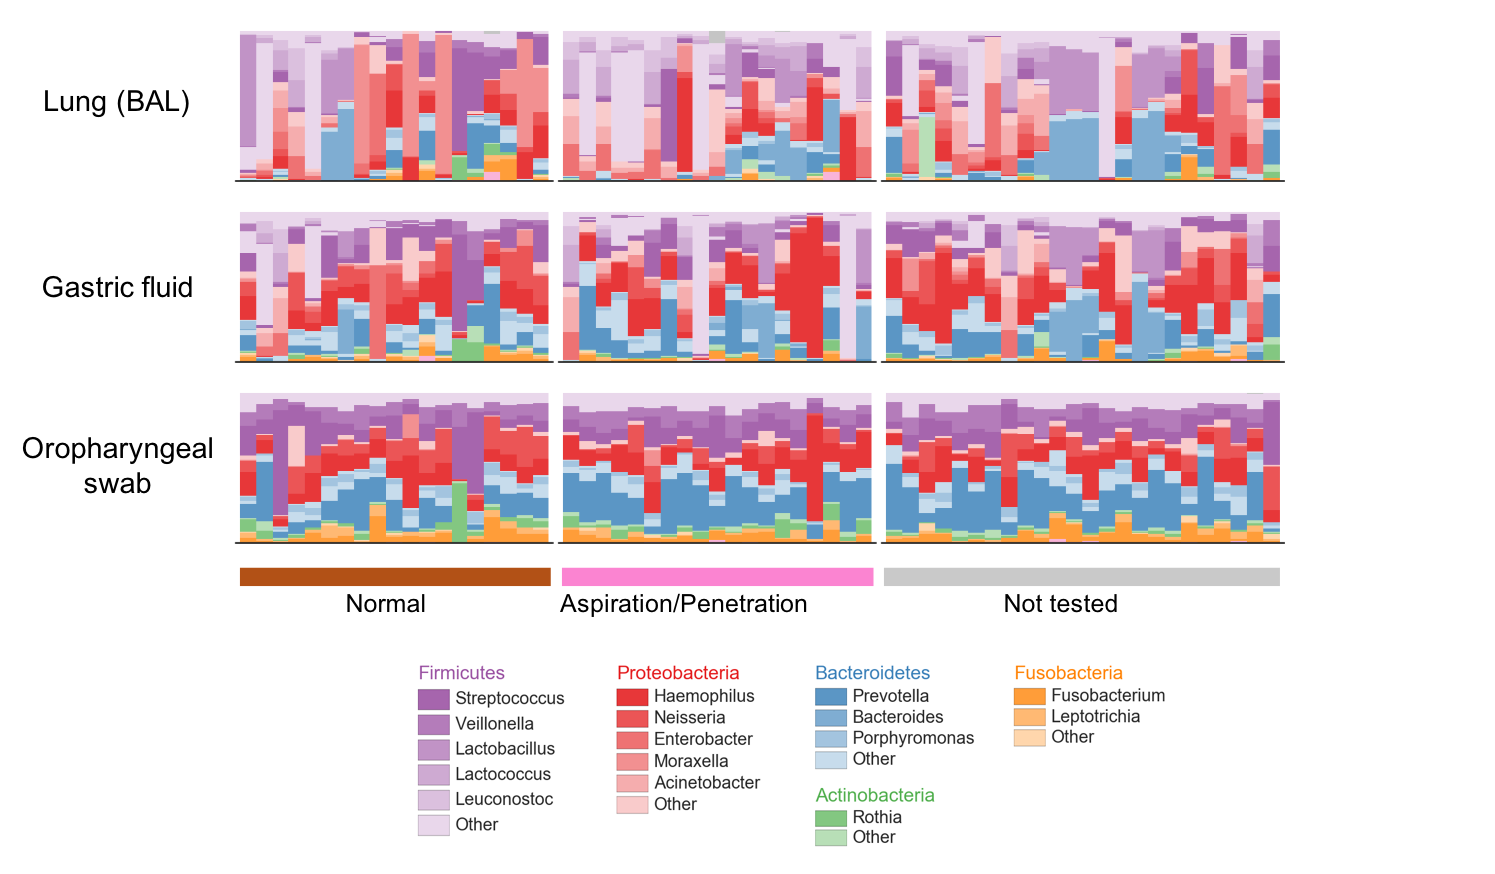
\includegraphics[width=1.2\textwidth]{community_overview_whitebckg.png}
        \caption{\textbf{Aerodigestive communities have similar predominant genera.} Bar plots showing relative abundances of aerodigestive OTUs collapsed to the genus level. Each column corresponds to one patient who had all three aerodigestive sites sequenced (N $=$ 19 non-aspirators, 23 aspirators, 24 untested). Phyla in legend are those with mean abundance $>$ 0.01 across all patients. Any other phyla are colored gray.}
        \label{fig1}
        \end{center}
\end{figure}

\begin{figure}[h]
        \begin{center}
        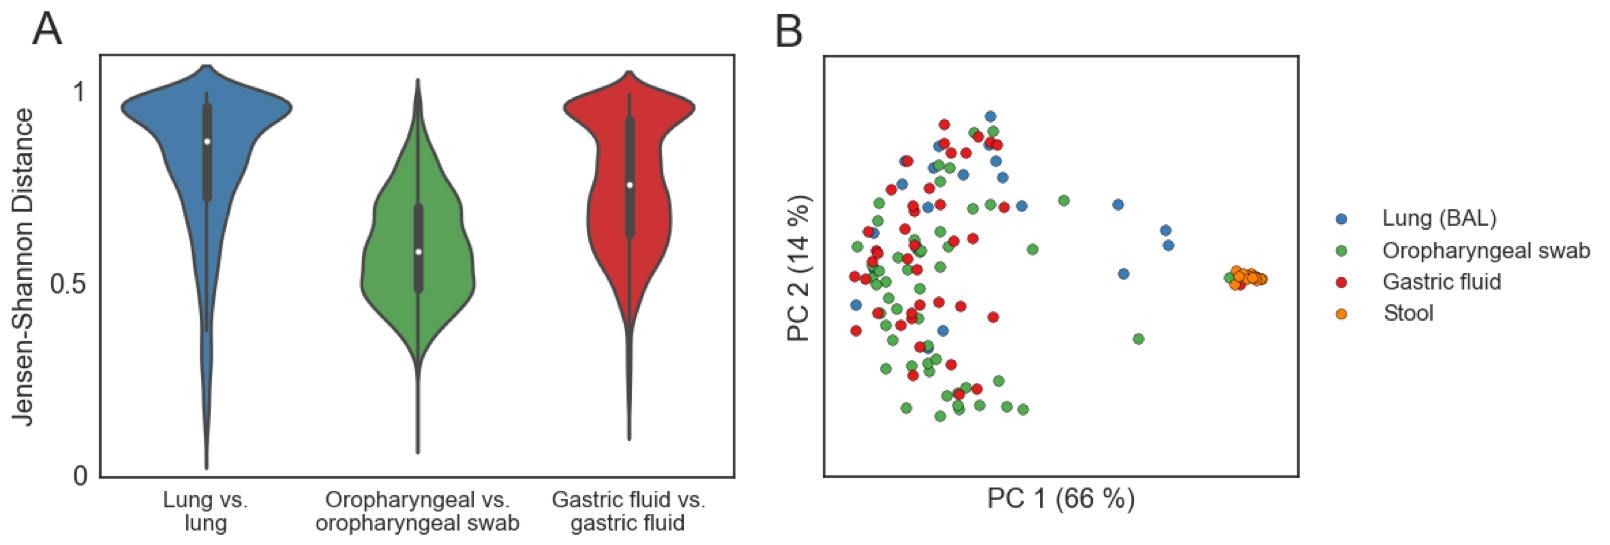
\includegraphics[width=\textwidth]{baseline_aerodigestive_across_patients_whitebckg.png}
        \caption{\textbf{Lung and gastric communities are more variable across people than oropharyngeal communities.} (A) Violin plot of the Jensen-Shannon distance (JSD) between samples from the same site across different patients. A JSD close to 1 indicates that communities are very different (less similar). (B) PCoA plots of aerodigestive and stool microbial communities for all patients in the 2016 sequencing batch (N $=$ 21 BAL, 52 oropharyngeal swab, 43 gastric fluid, and 14 stool samples).}
        \label{fig2}
        \end{center}
\end{figure}

\begin{figure}[h]
        \begin{center}
        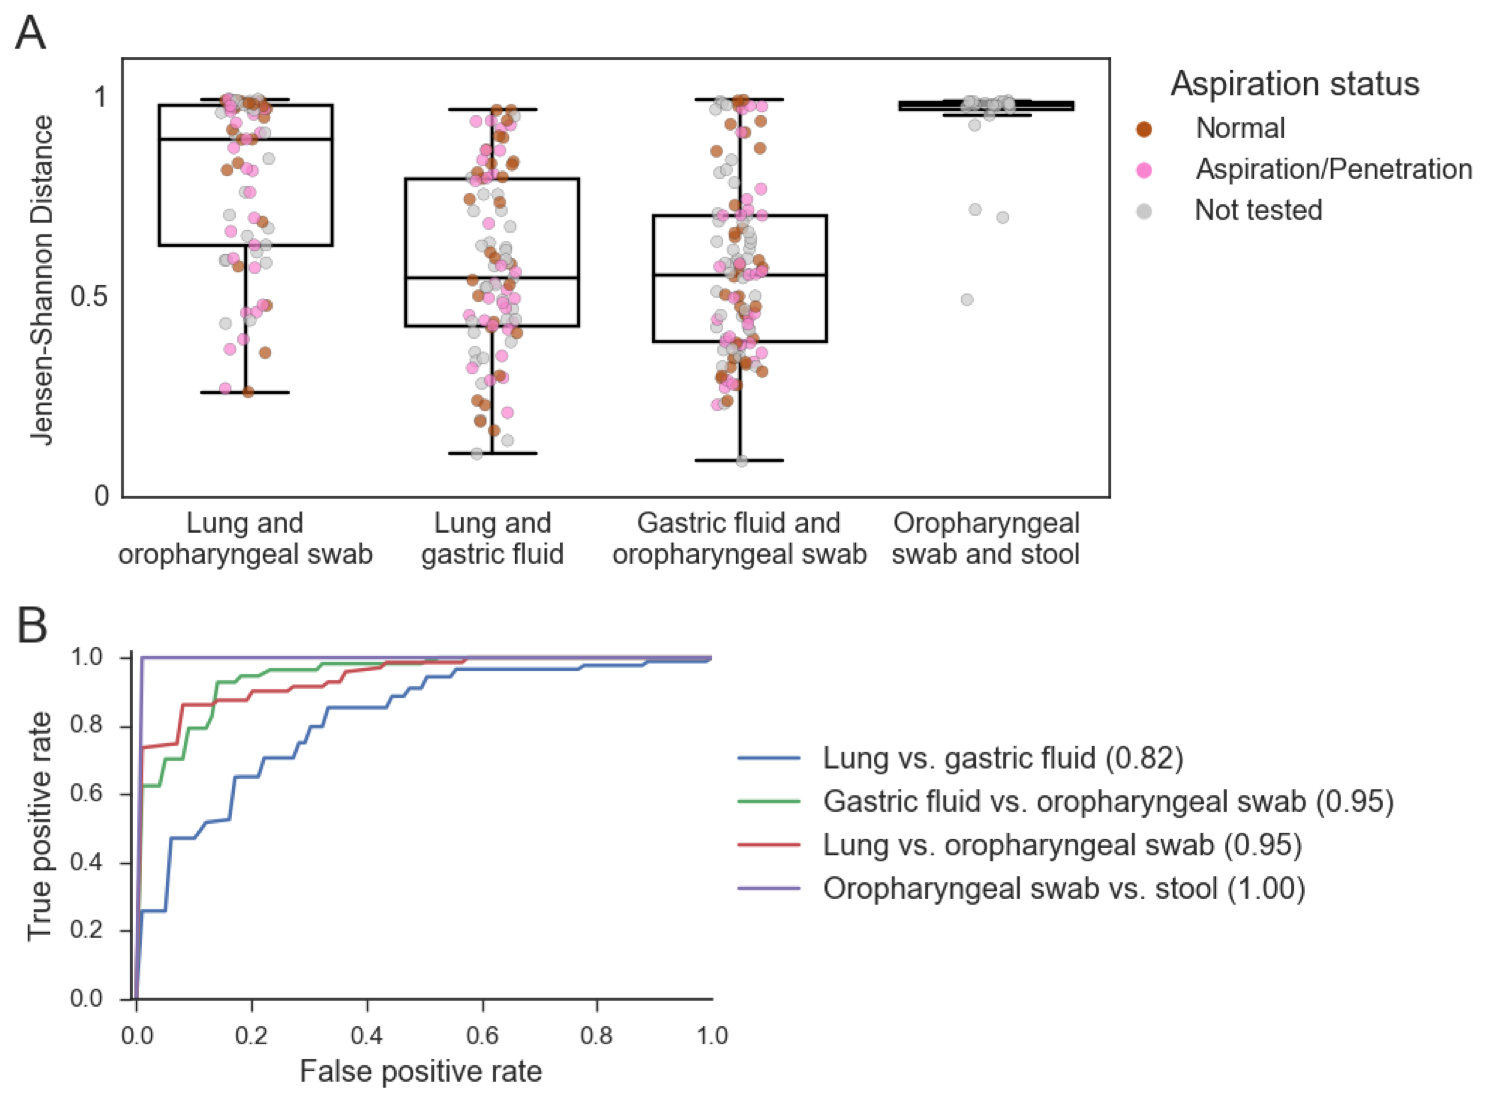
\includegraphics[width=\textwidth]{baseline_aerodigestive_within_patients_whitebckg.png}
        \caption{\textbf{Within patients, aerodigestive communities are similar but lung and oropharynx remain most distinct.} (A) Jensen-Shannon distances between samples from different sites from the same patient. Comparisons between stool and oropharynx are included to contextualize these results, as these are expected to be very different. All comparisons are significant (Wilcoxon rank sums test calculated with Python's \texttt{scipy.stats.ranksums} function) except the lung and gastric fluid vs. gastric fluid and oropharyngeal swab beta diversities (p $=$ 0.6). Lung and oropharyngeal vs. oropharyngeal and stool, p $=$ 0.005. All other comparisons:  $p < 1 \times 10^{-8}$. (B) ROC curve of classifiers distinguishing different aerodigestive sites. Mean areas under the ROC curve (AUCs) are reported in parentheses in the legend.}
        \label{fig3}
        \end{center}
\end{figure}

\begin{figure}[h]
        \begin{center}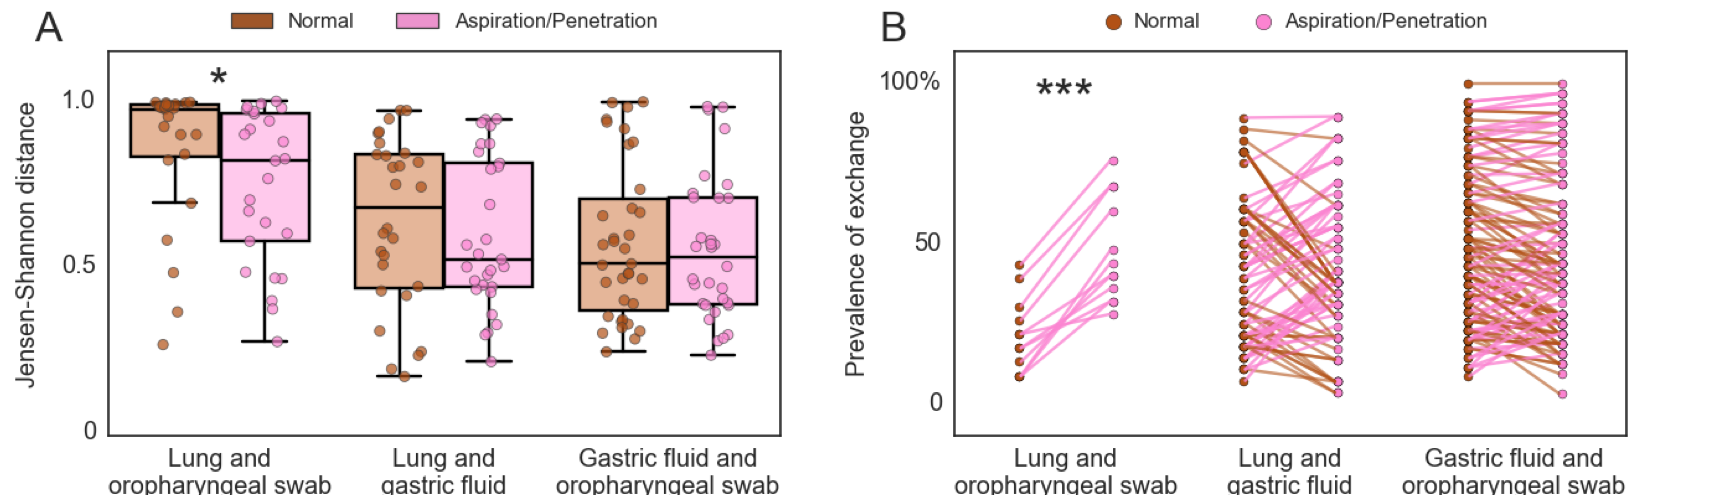
\includegraphics[width=\textwidth]{aspiration_jsd_exchange_whitebckg.png}
        \caption{\textbf{Dysphagia increases aspiration of microbes from the oropharynx but not the stomach} (A) Intra-patient Jensen Shannon distance for different aerodigestive site comparisons in non-aspirators (brown) and aspirators (pink). Each point represents one patient. P-values (Wilcoxon rank sums test, calculated with Python's \texttt{scipy.stats.ranksums} function): lung and oropharyngeal swab $p = 0.04$, lung and gastric fluid $p = 0.5$, gastric fluid and oropharyngeal swab $p = 0.8$. (B) Percentage of patients with the previously defined exchanged microbes present in both of the respective sites (x-axis) in non-aspirators (brown) and aspirators (pink). Each pair of points represents one exchanged OTU. P-values (paired t-test on $log_{10}$ prevalence values, calculated with Python's \texttt{scipy.stats.ttest\_rel} function: lung and oropharyngeal swab $p = 3 \times 10^{-5}$, lung and gastric fluid $p = 0.8$, gastric fluid and oropharyngeal swab $p = 0.09$.}
        \label{fig4}
        \end{center}
\end{figure}

\begin{figure}[h]
        \begin{center}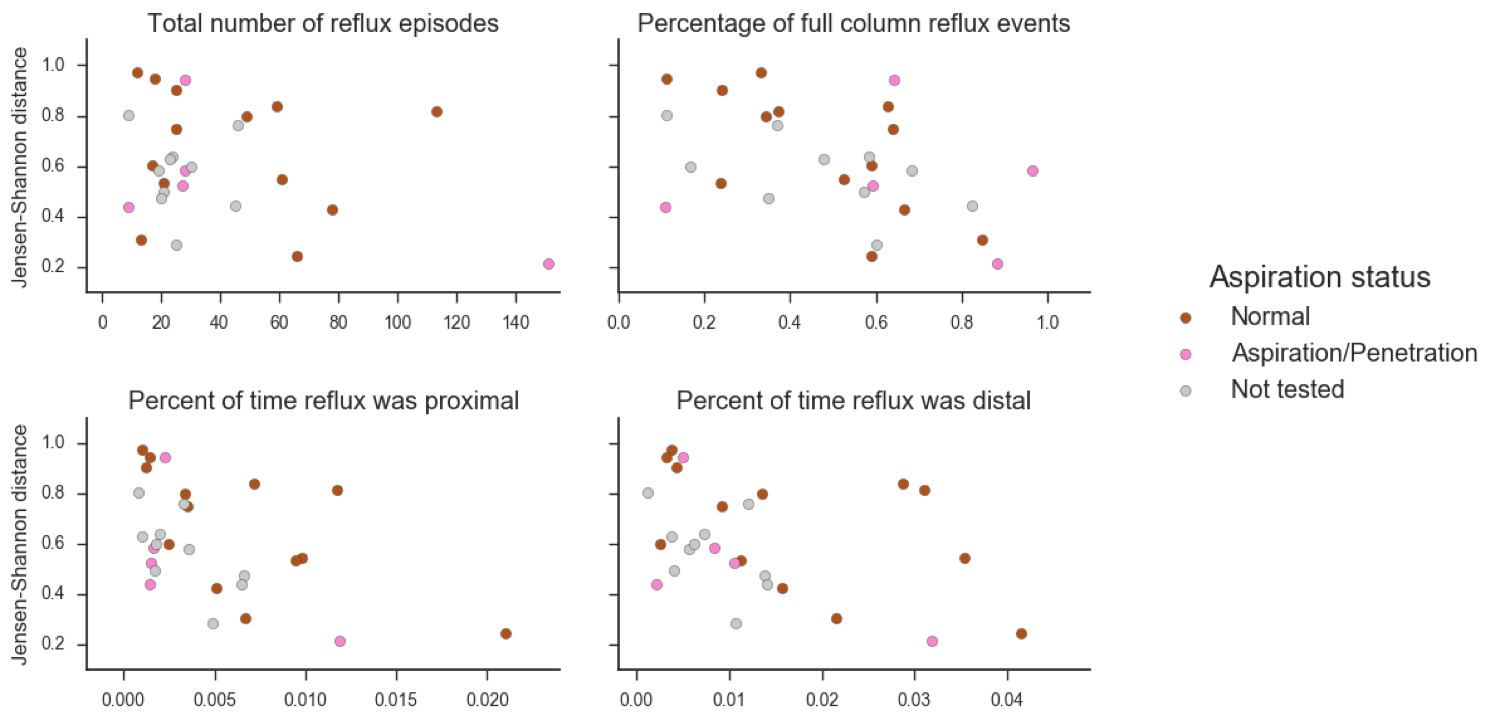
\includegraphics[width=\textwidth]{reflux_correlation_with_bal_gastric.png}
        \caption{\textbf{Reflux severity may correlate with the similarity between lung and gastric communities.} Each plot shows the correlation between different reflux measures and the within-patient Jensen-Shannon distance between BAL and gastric fluid samples. Points are colored according to aspiration status. All reflux measures include both acid- and non-acid reflux. Spearman correlation and p-values: total number of reflux episodes $\rho_s = -0.14, p = 0.5$, percentage of full column reflux events $\rho_s = -0.41, p = 0.03$, percent of time reflux was proximal $\rho_s = -0.47, p = 0.01$, percent of time reflux was distal $\rho_s = -0.43, p = 0.02$.}
        \label{fig5}
        \end{center}
\end{figure}

\FloatBarrier
\newpage

\bibliographystyle{unsrtnat}
\bibliography{aspiration/aspiration_refs.bib}

%\end{document}


\clearpage

\section{Figures}

\begin{figure}[h]
        \begin{center}
        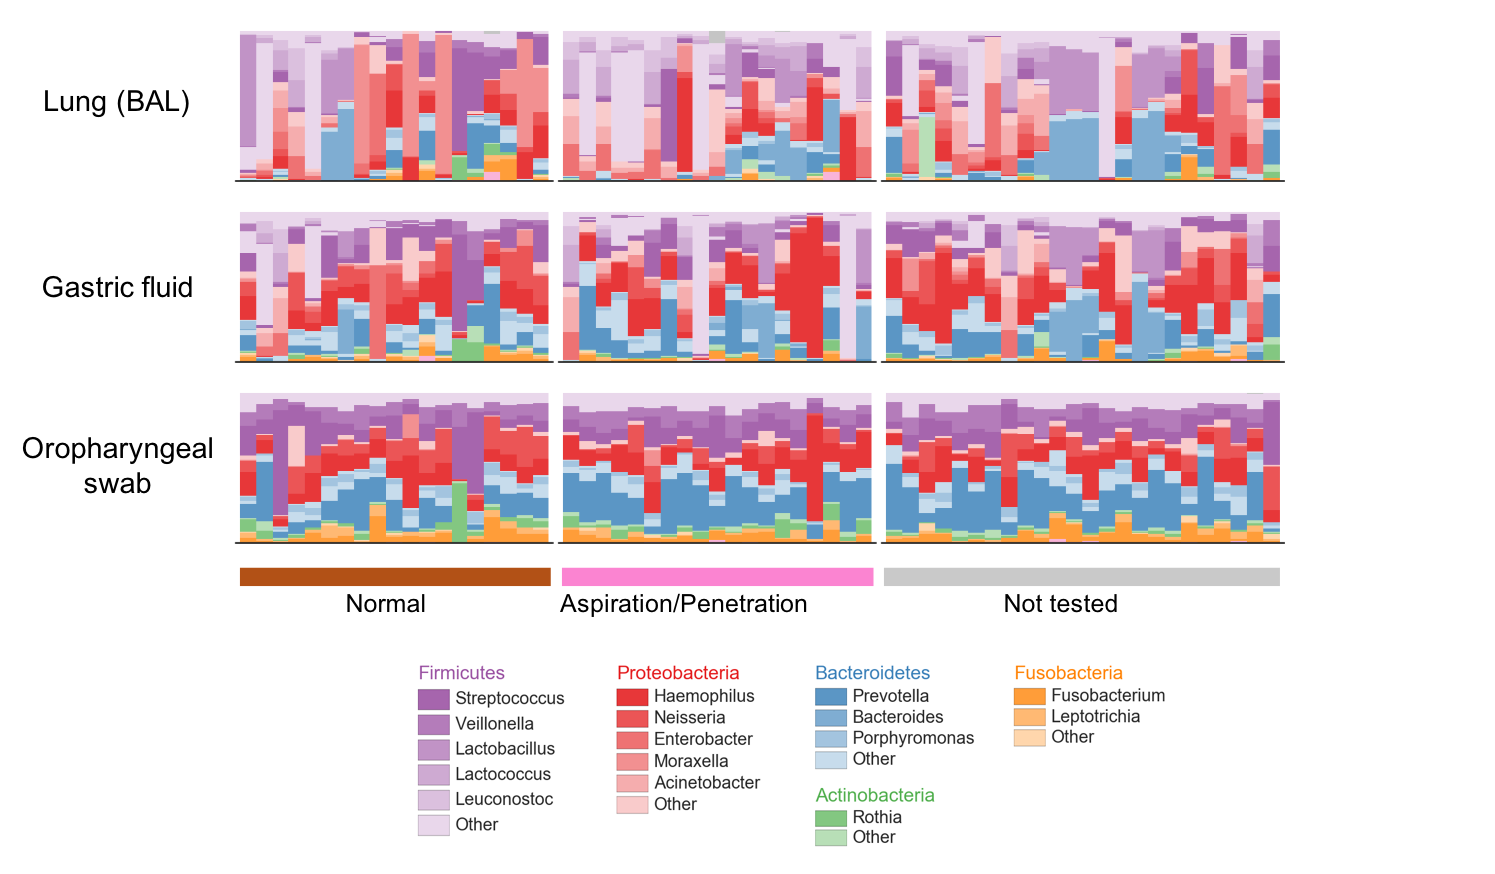
\includegraphics[width=1.2\textwidth]{community_overview_whitebckg.png}
        \caption{\textbf{Aerodigestive communities have similar predominant genera.} Bar plots showing relative abundances of aerodigestive OTUs collapsed to the genus level. Each column corresponds to one patient who had all three aerodigestive sites sequenced (N $=$ 19 non-aspirators, 23 aspirators, 24 untested). Phyla in legend are those with mean abundance $>$ 0.01 across all patients. Any other phyla are colored gray.}
        \label{fig:overview_plots}
        \end{center}
\end{figure}

\begin{figure}[h]
        \begin{center}
        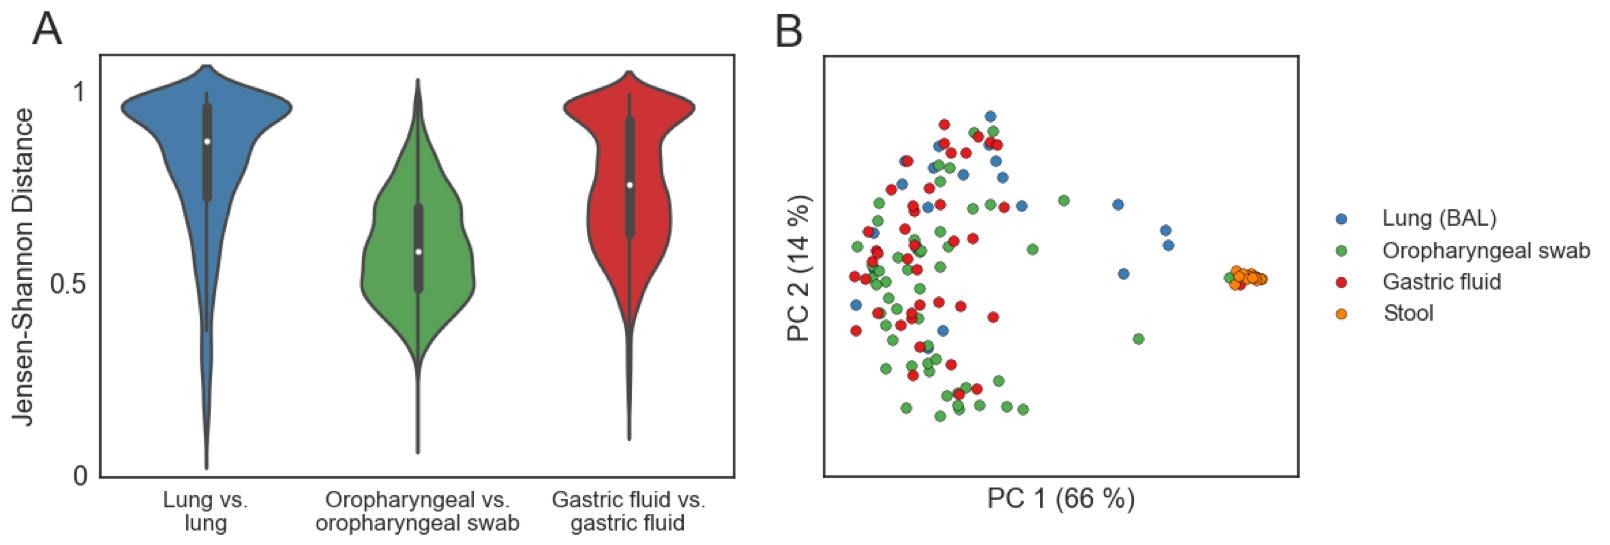
\includegraphics[width=\textwidth]{baseline_aerodigestive_across_patients_whitebckg.png}
        \caption{\textbf{Lung and gastric communities are more variable across people than oropharyngeal communities.} (A) Violin plot of the Jensen-Shannon distance (JSD) between samples from the same site across different patients. A JSD close to 1 indicates that communities are very different (less similar). (B) PCoA plots of aerodigestive and stool microbial communities for all patients in the 2016 sequencing batch (N $=$ 21 BAL, 52 oropharyngeal swab, 43 gastric fluid, and 14 stool samples).}
        \label{fig:across_people}
        \end{center}
\end{figure}

\begin{figure}[h]
        \begin{center}
        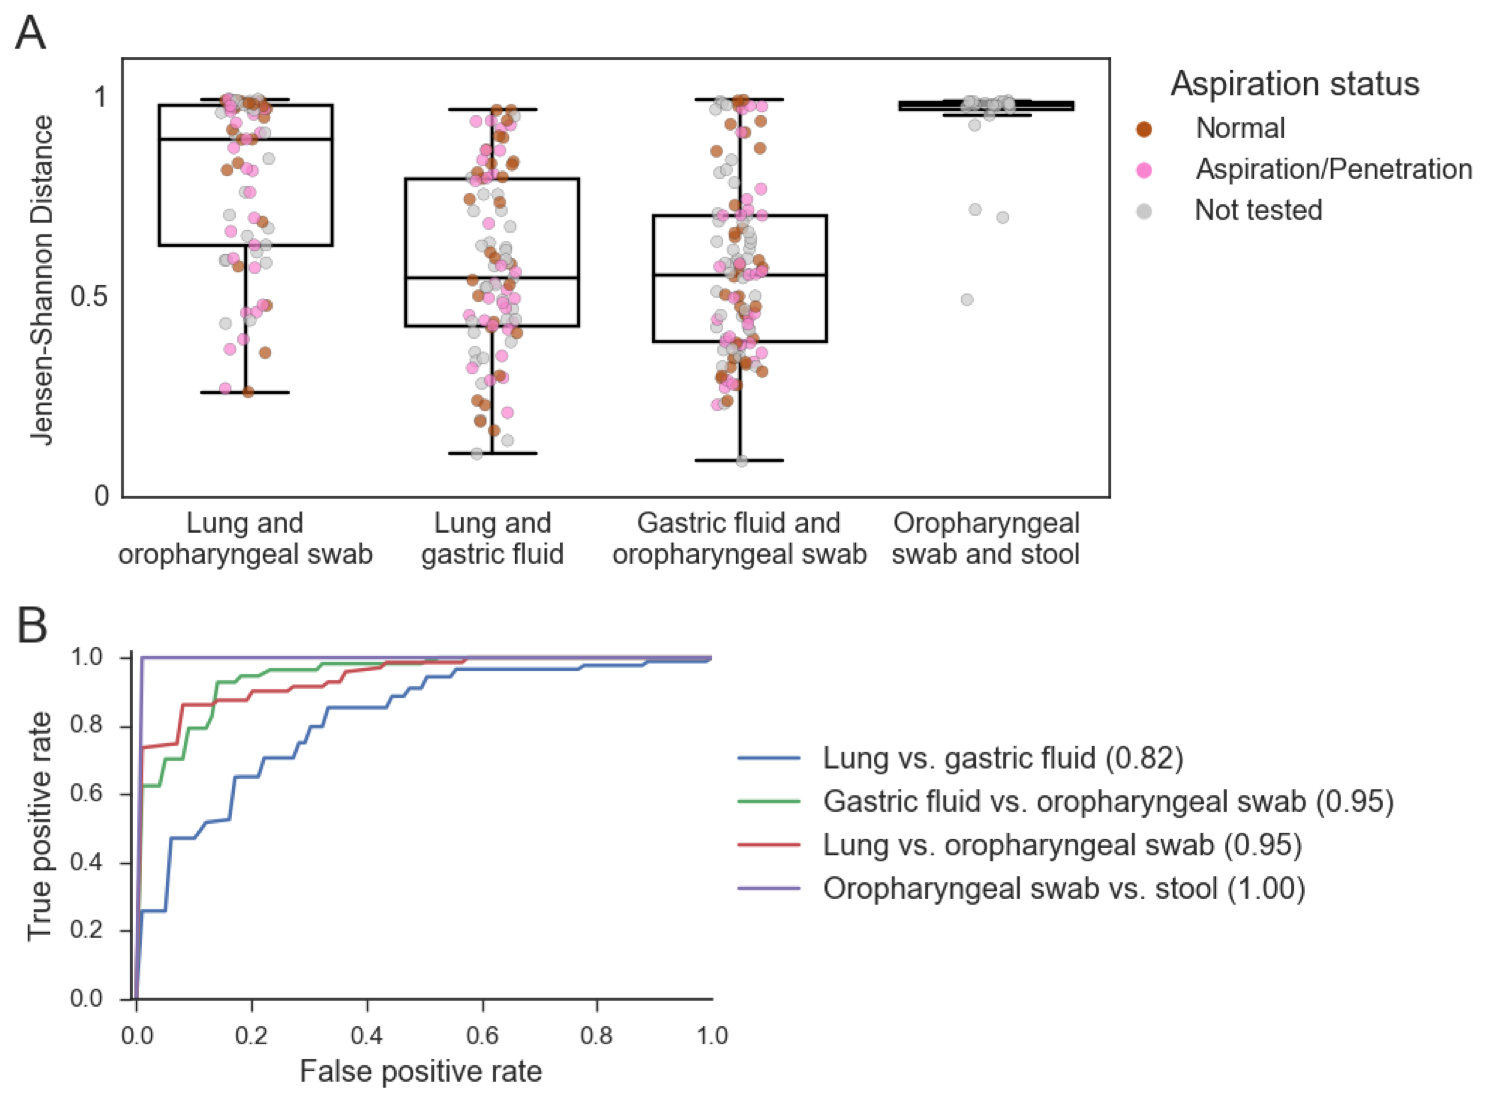
\includegraphics[width=\textwidth]{baseline_aerodigestive_within_patients_whitebckg.png}
        \caption{\textbf{Within patients, aerodigestive communities are similar but lung and oropharynx remain most distinct.} (A) Jensen-Shannon distances between samples from different sites from the same patient. Comparisons between stool and oropharynx are included to contextualize these results, as these are expected to be very different. All comparisons are significant (Wilcoxon rank sums test calculated with Python's \texttt{scipy.stats.ranksums} function) except the lung and gastric fluid vs. gastric fluid and oropharyngeal swab beta diversities (p $=$ 0.6). Lung and oropharyngeal vs. oropharyngeal and stool, p $=$ 0.005. All other comparisons:  $p < 1 \times 10^{-8}$. (B) ROC curve of classifiers distinguishing different aerodigestive sites. Mean areas under the ROC curve (AUCs) are reported in parentheses in the legend.}
        \label{fig:within_patients}
        \end{center}
\end{figure}

\begin{figure}[h]
        \begin{center}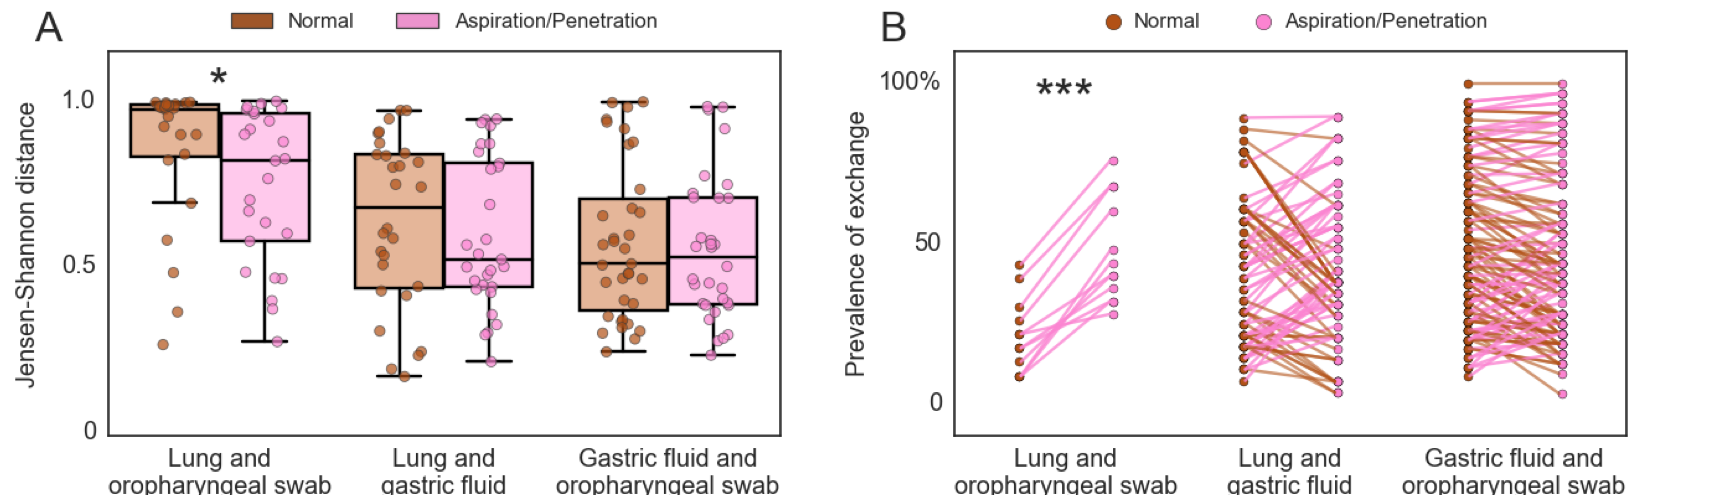
\includegraphics[width=\textwidth]{aspiration_jsd_exchange_whitebckg.png}
        \caption{\textbf{Dysphagia increases aspiration of microbes from the oropharynx but not the stomach} (A) Intra-patient Jensen Shannon distance for different aerodigestive site comparisons in non-aspirators (brown) and aspirators (pink). Each point represents one patient. P-values (Wilcoxon rank sums test, calculated with Python's \texttt{scipy.stats.ranksums} function): lung and oropharyngeal swab $p = 0.04$, lung and gastric fluid $p = 0.5$, gastric fluid and oropharyngeal swab $p = 0.8$. (B) Percentage of patients with the previously defined exchanged microbes present in both of the respective sites (x-axis) in non-aspirators (brown) and aspirators (pink). Each pair of points represents one exchanged OTU. P-values (paired t-test on $log_{10}$ prevalence values, calculated with Python's \texttt{scipy.stats.ttest\_rel} function: lung and oropharyngeal swab $p = 3 \times 10^{-5}$, lung and gastric fluid $p = 0.8$, gastric fluid and oropharyngeal swab $p = 0.09$.}
        \label{fig:aspiration}
        \end{center}
\end{figure}

\begin{figure}[h]
        \begin{center}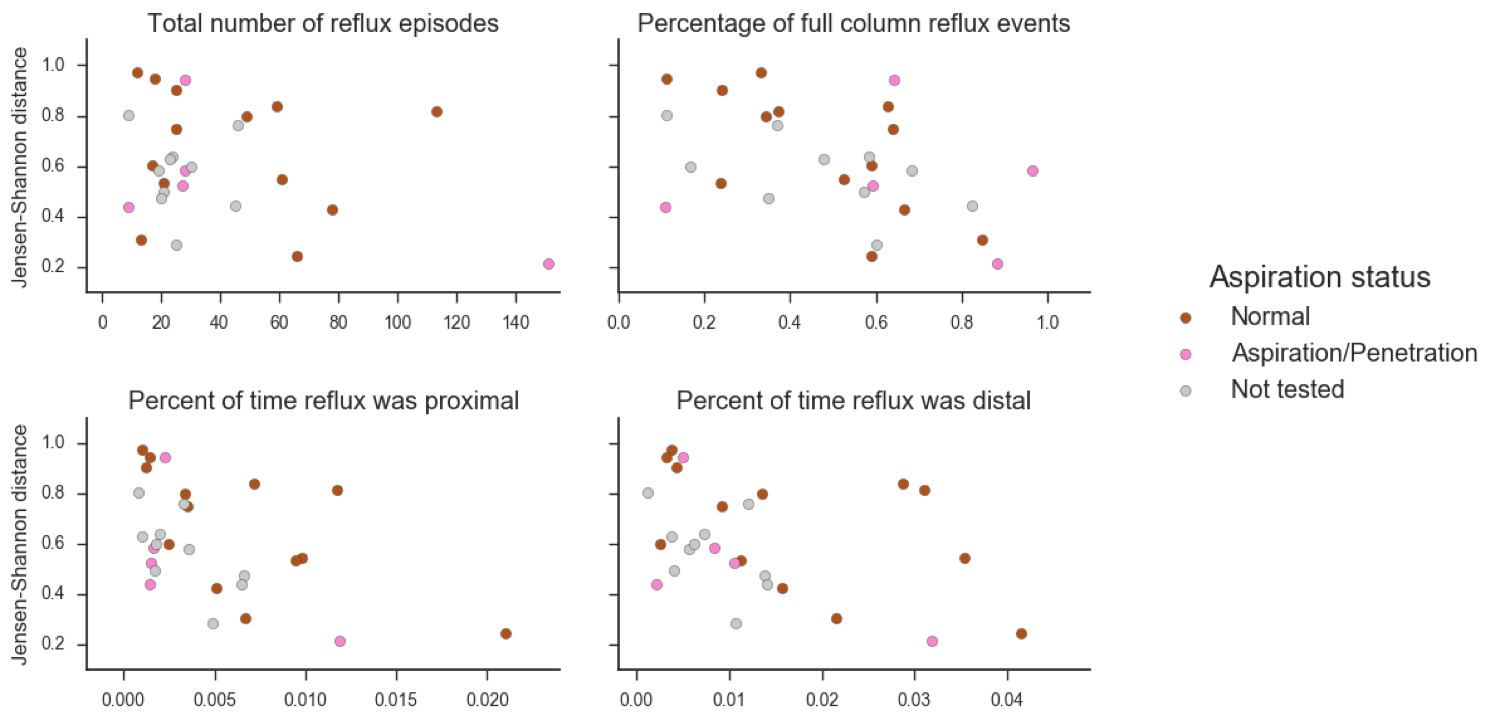
\includegraphics[width=\textwidth]{reflux_correlation_with_bal_gastric.png}
        \caption{\textbf{Reflux severity may correlate with the similarity between lung and gastric communities.} Each plot shows the correlation between different reflux measures and the within-patient Jensen-Shannon distance between BAL and gastric fluid samples. Points are colored according to aspiration status. All reflux measures include both acid- and non-acid reflux. Spearman correlation and p-values: total number of reflux episodes $\rho_s = -0.14, p = 0.5$, percentage of full column reflux events $\rho_s = -0.41, p = 0.03$, percent of time reflux was proximal $\rho_s = -0.47, p = 0.01$, percent of time reflux was distal $\rho_s = -0.43, p = 0.02$.}
        \label{fig:reflux_corr}
        \end{center}
\end{figure}


%TODO: need to add references to the figures in the aspiration main.text (or just put the figures in that file)

%% This is an example first chapter.  You should put chapter/appendix that you
%% write into a separate file, and add a line \include{yourfilename} to
%% main.tex, where `yourfilename.tex' is the name of the chapter/appendix file.
%% You can process specific files by typing their names in at the
%% \files=
%% prompt when you run the file main.tex through LaTeX.

\graphicspath{{meta-analysis/figures/}}

\chapter{Meta-analysis of gut microbiome studies identifies disease-specific and shared responses}

The contents of this chapter were published as:

Claire Duvallet, Sean M. Gibbons, Thomas Gurry, Rafael A. Irizarry, and Eric J. Alm. "Meta-analysis of gut microbiome studies identifies disease-specific and shared responses." \textit{Nature Communications}. (2017)

The figures are at the end of the chapter. The Supplementary Information is in Appendix B.

\clearpage

%\usepackage[colorlinks=true]{hyperref} % for links and urls
%\usepackage{amsmath,amssymb} % for math
%\usepackage{color,soul} % for highlighting
%\usepackage{booktabs,rotating,multirow} % for nice tables
%\usepackage{authblk} % for author affiliations
%\usepackage{graphicx} % for figures
%\usepackage[numbers]{natbib}
%\usepackage[superscript,biblabel]{cite} % for superscript citations
%\usepackage[above]{placeins} % for FloatBarrier
%\usepackage{amsmath} % for pretty fraction text (heatmap caption)
%\usepackage{lineno} % for line numbers
%\usepackage{geometry} % for supp fig large pages

%% Smaller captions
%\usepackage[font=footnotesize]{caption}

\section*{Abstract}
Hundreds of clinical studies have demonstrated associations between the human microbiome and disease, yet fundamental questions remain on how we can generalize this knowledge.
Results from individual studies can be inconsistent and comparing published data is further complicated by a lack of standard processing and analysis methods.
Here, we introduce the MicrobiomeHD database, which includes 28 published case-control gut microbiome studies spanning ten diseases.
We perform a cross-disease meta-analysis of these studies using standardized methods.
We find consistent patterns characterizing disease-associated microbiome changes.
Some diseases are associated with over 50 genera, while most show only 10 to 15 genus-level changes.
Some diseases are marked by the presence of potentially pathogenic microbes whereas others are characterized by a depletion of health-associated bacteria.
Furthermore, we show that about half of genera associated with individual studies are bacteria which respond to more than one disease.
Thus, many associations found in case-control studies are likely not disease-specific but rather part of a non-specific, shared response to health and disease.

\newpage

\section{Introduction}

The human gastrointestinal tract digests food, absorbs nutrients, and plays important roles in maintaining metabolic homeostasis.
The microbes residing in our gut harvest energy from the food we eat, train our immune system, break down xenobiotics and other foreign products, and release metabolites and hormones important for regulating our physiology \cite{nash-baker, asd-kb, turnbaugh2006obesity}.
Chemical signals from our microbiota can act locally within the gut, and can also have larger systemic effects (e.g. the `gut-brain axis') \cite{Hsiao2013gutbrain,Cryan2012gutbrain,Poutahidis2013gutbrain}.

Due to the physiological interplay between humans and our microbial communities, many diseases are hypothesized to be associated with shifts away from a ``healthy'' gut microbiome.
These include metabolic disorders, inflammatory and auto-immune diseases, neurological conditions, and cancer, among others \cite{nash-baker, turnbaugh2006obesity, asd-son, crc-zhao, par-schep}.
Certain gut-related conditions (e.g. obesity and inflammatory bowel disease) have been extensively studied in human cohorts and in animal experiments, where significant and sometimes causal microbial associations have been shown.
These studies have spurred research into a number of complex diseases with unclear etiologies where a connection to the microbiome is suspected.

Overall, our current understanding of the precise relationships between the human gut microbiome and disease remains limited.
Existing case-control studies often report finding disease-associated microbial ``dysbiosis''.
However, the term ``dysbiosis'' is inconsistently and often vaguely defined, and can have a wide range of interpretations \cite{olesen2016dysbiosis,zaneveld2017karenina}.
Thus, we lack a comprehensive understanding of precisely how microbial communities and specific microbes within those communities cause, respond to, or contribute to disease.
Are different diseases characterized by distinct shifts in the gut microbiome?
Are some diseases marked by an invasion of pathogens whereas others show a depletion of beneficial bacteria?
Can we identify microbial biomarkers for certain conditions, which are consistently enriched or depleted in a disease across many patient cohorts?
Finally, are some bacteria part of a non-specific ``healthy'' or ``diseased'' microbiome and consistently associated with health or disease in general?

One approach to synthesize existing knowledge is to identify consistencies across studies through a meta-analysis, which allows researchers to find and remove false positives and negatives that may obscure underlying biological patterns.
However, prior meta-analyses of case-control gut microbiome studies have yielded mixed results and did not contextualize their findings across multiple diseases \cite{walters2014meta, Sze07092016,finucane2014obesity}.
For some conditions like inflammatory bowel disease (IBD), an overall difference in the gut microbiota was found within several studies, but no individual microbes were consistently associated with IBD across studies \cite{walters2014meta}.
For other conditions like obesity, multiple meta-analyses have found little to no difference in the gut microbiomes of obese and lean patients \cite{walters2014meta,Sze07092016,finucane2014obesity}, even though the microbiome has been causally linked to obesity in mouse models \cite{turnbaugh2006obesity, ridaura2013gut}.
These meta-analyses have been limited by focusing on only one or two diseases, and thus do not extend their findings across a broader landscape of human disease to answer more general questions about overall patterns of disease-associated microbiome shifts.

In this paper, we collected 28 published case-control 16S amplicon sequencing gut microbiome datasets spanning ten different disease states.
We acquired raw data and disease metadata for each study and systematically re-processed and re-analyzed the data.
We investigated whether consistent and specific disease-associated changes in gut microbial communities could be identified across multiple studies of the same disease.
Certain diseases (e.g. colorectal cancer (CRC)) are marked by an enrichment of disease-associated bacteria, while others (e.g. IBD) are characterized by a depletion of health-associated bacteria.
Some conditions (e.g. diarrhea) exhibit large-scale community shifts with many associated microbes, while most show only a handful of associations.
However, many associations are not specific to individual diseases but rather respond to multiple disease states.
In most studies, the majority of the individual disease-associated microbes were part of this set of bacteria that respond non-specifically to healthy and diseased states.
Thus, associations from individual case-control studies should be interpreted with caution, as these microbes may be indicative of a shared response to disease rather than part of disease-specific differences.
Together, these findings reveal distinct categories of dysbioses which can inform the development of microbiome-based diagnostics and therapeutics.

\section{Results}

\subsection{Most disease states show altered microbiomes}

To answer questions about the reproducibility and generalizability of reported associations between the human microbiome and disease, we collected, re-processed, and re-analyzed raw data from a collection of microbiome datasets.
We included studies with publicly available 16S amplicon sequencing data (i.e. FASTQ or FASTA) for stool samples from at least 15 case patients which also had associated disease metadata (i.e. case or control disease labels).
Studies which exclusively focused on children under 5 years old were excluded from our analyses.
We identified over 50 suitable case-control 16S datasets, of which 28 were successfully downloaded, processed, and included in a publicly available database which we called MicrobiomeHD \cite{microbiomehd}.
Characteristics of these datasets, including sample sizes, diseases and conditions, and references, are shown in Table \ref{tab:datasets} and Supplementary Table \ref{tab:datasets_full_info}.
For each downloaded study, we processed the raw sequencing data through our 16S processing pipeline (\url{https://github.com/thomasgurry/amplicon_sequencing_pipeline}) (see Supplementary Tables \ref{tab:processing} and \ref{tab:data} for detailed data sources and processing methods).
100\% denovo OTUs were assigned taxonomy with the RDP classifier \cite{wang2007naive} (c $=$ 0.5), converted to relative abundances by dividing by total sample reads, and collapsed to the genus level. OTUs which were not assigned at the genus level were discarded.
By collapsing data to the genus level, we lost the sensitivity to detect fine-scale differences in species or strain abundances across case and control groups, but we minimized certain batch effects that plague comparisons across studies.
Thus, we took a course-grained approach to optimize our ability to compare data across studies at the expense of phylogenetic resolution.

We first asked whether reported associations between the gut microbiome and disease would be recapitulated once we controlled for processing and analysis approaches.
To test whether the gut microbiome is altered in a variety of disease states, we built genus-level random forest classifiers to classify cases from controls within each study.
We compared the resulting area under the Receiver Operating Characteristic (ROC) curves (AUC) across studies (Figure \ref{fig:fig1}A, Supplementary Figure \ref{fig:roc_curves}).
We could classify cases from controls (AUC $>$ 0.7) for at least one dataset for all diseases except arthritis and Parkinson's disease, which each only had one study.
Notably, all diarrhea datasets (except Youngster et al. (2014) \cite{cdi-youngster}, which had only 4 distinct control patients and thus was not included in this analysis) had very high classifiability (AUC $>$ 0.9).
We successfully classified patients from controls (AUC $>$ 0.7) in three out of four IBD studies and all four CRC studies, which is consistent with previous work showing that these patients can be readily distinguished from controls using supervised classification methods \cite{walters2014meta,ibd-papa,crc-baxter,crc-zeller}.
Thus, the microbiome is indeed altered in many different diseases.

\subsection{Loss of beneficial microbes or enrichment of pathogens}

We next wondered whether the specific type of alteration was consistent across independent cohorts of patients with the same disease.
We performed univariate tests on genus-level relative abundances for each dataset independently and compared results across studies (Kruskal-Wallis (KW) test with the Benjamini-Hochberg false discovery rate (FDR) correction \cite{benjamini-hochberg}).
Our re-analyses of the studies were largely consistent with the originally reported results.
The same taxonomic groups showed similar trends as in the original publications, despite differences in data-processing methodologies (see Supplementary Note \ref{sec:lit_comp} for a full comparison of our re-analysis with previously published results).
Furthermore, we found that the disease-associated changes in the microbiome could be categorized into meaningful groups which provide insight into possible etiologies or therapeutic strategies for different types of disease.

In some diseases, microbiome shifts are dominated by an enrichment of a small number of ``pathogenic'' bacteria.
In these cases, it is possible that the microbes play a causal role and that they could be targeted with narrow-spectrum antimicrobials.
Colorectal cancer is characterized by such a shift, and we found significant agreement across three of the four CRC studies \cite{crc-zhao,crc-baxter,crc-zeller,crc-xiang} (Figures \ref{fig:fig1}B and \ref{fig:fig2}, genus labels in Supplementary Figure \ref{fig:supp_dis_specific}).
Dysbiosis associated with CRC is generally characterized by increased prevalence of the known pathogenic or pathogen-associated \textit{Fusobacterium}, \textit{Porphyromonas}, \textit{Peptostreptococcus}, \textit{Parvimonas}, and \textit{Enterobacter} genera (i.e. these genera were higher in CRC patients in 2 or more studies, Figures \ref{fig:fig2} and \ref{fig:fig3}A, genus labels in Supplementary Figures \ref{fig:supp_dis_specific} and \ref{fig:supp_meta_heatmap}).
\textit{Fusobacterium} is associated with a broad spectrum of human diseases and \textit{Porphyromonas} is a known oral pathogen \cite{Han2015fusopatho, Flynn2016oral}.

By contrast, other disease-associated microbiome shifts are characterized by a depletion of health-associated bacteria in patients relative to controls.
In these cases, probiotics that replace missing taxa may be a better treatment strategy than anti-microbials.
Across our four IBD studies, patient microbiomes were dominated by a depletion of genera in patients relative to controls, especially butyrate-producing \textit{Clostridiales} \cite{ibd-papa,ibd-gevers,ibd-hut,ibd-engstrand} (Figures \ref{fig:fig1}B and \ref{fig:fig2}, genus labels in Supplementary Figure \ref{fig:supp_dis_specific}).
In particular, five genera from the \textit{Ruminococcacaea} and \textit{Lachnospiracaea} families were consistently depleted in IBD patients relative to controls in at least two studies (Figure \ref{fig:fig3}A, genus labels in Supplementary Figure \ref{fig:supp_meta_heatmap}).
While not all genera within \textit{Ruminococcacaea} and \textit{Lachnospiracaea} are verified short-chain fatty acid (SCFA) producers, the dominant genera within these families are known to harbor genes for short chain fatty acid production \cite{louis2010diversity} and are often associated with colonic health \cite{flint2012role,miquel2013faecalibacterium,reeves2012suppression}.
We found similar results when comparing Crohn's disease and ulcerative colitis patients to controls separately, without any consistent patterns across datasets that distinguished either IBD sub-type (Supplementary Note \ref{sec:split_cases}; Supplementary Figures \ref{fig:split_cases_fig1} and \ref{fig:split_cases_heatmaps}).

Some conditions are characterized by a broad restructuring of gut microbial communities.
In these cases, full community restoration strategies like fecal microbiota transplants may be more appropriate.
For example, diarrhea consistently results in large-scale rearrangements in the composition of the gut microbiome, which is likely reflective of reduced stool transit time (Figures \ref{fig:fig1} and \ref{fig:fig2}).
We saw many microbes consistently associated with both \textit{Clostridium difficile} infection (CDI) and non-CDI diarrhea (Figures \ref{fig:fig2} and \ref{fig:fig3}A) \cite{cdi-youngster,cdi-schubert,cdi-vincent,edd-singh}.
In general, Proteobacteria increase in prevalence in patients with diarrhea, with a concomitant decrease in the relative abundances of Bacteroidetes and some Firmicutes.
In particular, we see a reduction in butyrate-producing Clostridia, including genera within \textit{Ruminococcaceae} and \textit{Lachnospiraceae} families, which have been associated with a healthy gut \cite{wong2006colonic}.
We also see an increase in prevalence of genera that contain organisms often associated with lower pH and higher oxygen levels of the upper-gut, like \textit{Lactobacillaceae} and \textit{Enterobacteriaceae}, in patients with diarrhea (Figure \ref{fig:fig3}A) \cite{donaldson2016gut}.
Additionally, both CDI and non-CDI diarrhea patients had lower alpha diversity, a measure of overall community structure, than healthy controls in all studies (Supplementary Figures \ref{fig:fig_alpha}-\ref{fig:fig_alpha_simpson}).
Consistent with the CDI and non-CDI diarrheal studies, we also found that organisms associated with the upper gut, like \textit{Lactobacillus} and \textit{Enterobacteriaceae}, appear to be enriched in IBD patients, who can present with diarrheal symptoms (Supplementary Figure \ref{fig:supp_dis_specific}) \cite{donaldson2016gut,Kirsner1982ibd}.
IBD patients also tended to have lower alpha diversities than controls (Crohn's disease vs. controls in three studies, ulcerative colitis vs. controls in two studies; Supplementary Figures \ref{fig:fig_alpha}--\ref{fig:fig_alpha_simpson}), though this difference was less drastic than in the diarrheal studies where all patients had active diarrhea.

In some studies, confounding variables may drive associations.
For example, there were no consistent differences between cases and controls across HIV studies because of demonstrated confounders \cite{noguera2016gut,lozupone2013alterations,hiv-dinh} (Figure \ref{fig:fig2}, \ref{fig:fig3}A).
As in the original Lozupone et al. (2013) \cite{lozupone2013alterations} study, we found enrichment in \textit{Prevotella}, \textit{Catenibacterium}, \textit{Dialister}, and \textit{Desulfovibrio} in HIV-positive patients, in addition to 8 other genera (Figure \ref{fig:fig2} and Supplementary Figure \ref{fig:supp_dis_specific}).
We also found depletion of \textit{Bacteroides}, \textit{Odoribacter}, \textit{Anaerostipes}, \textit{Parasutterella}, and \textit{Alistipes} in HIV-positive patients relative to controls.
However, the Noguera-Julian et al. (2016) study showed that the genera that were significantly associated with HIV in the Lozupone paper were strongly associated with sexual behavior (e.g. men who have sex with men were associated with much higher \textit{Prevotella} levels), and our re-analysis also found conflicting results between these two studies (Figure \ref{fig:fig2}).
Thus, there is no consensus on what genera are associated with HIV.
Obesity is another example where confounding variables may drive microbiome alterations.
Three recent meta-analyses found no reproducible obesity-associated microbiome shifts \cite{walters2014meta,Sze07092016,finucane2014obesity}, which is consistent with our classification results where we were only able to accurately classify obese and control patients in two out of five studies (Zhu et al. (2013) \cite{nash-baker}, Turnbaugh et al. (2009) \cite{ob-gordon}; Figure \ref{fig:fig1}A).
Our genus-level re-analysis did find a few consistent genus-level associations between lean and obese patients \cite{nash-baker,ob-gordon,ob-goodrich,ob-zupancic,ob-ross}.
Two genera, \textit{Roseburia} and \textit{Mogibacterium}, were significantly enriched in obese individuals across two of the obesity studies (Figure \ref{fig:fig3}A).
Furthermore, \textit{Anaerovorax}, \textit{Oscillibacter}, \textit{Pseudoflavonifractor}, and \textit{Clostridium IV}  were depleted in obese patients relative to controls in two of the studies.
However, two of the five studies had no significant genus-level associations (q $<$ 0.05), despite one having a large sample size (Zupancic et al. (2012) \cite{ob-zupancic}).
This suggests that confounding factors like diet may have given rise to certain associations found in our re-analysis and previously reported in the literature \cite{finucane2014obesity}.
More studies that control for potential confounders, like host behavior and diet, will be required for diseases like obesity and HIV, where associations with the microbiome remain unclear.
Finally, patients in case-control cohorts are frequently on other medications such as antibiotics which may confound disease-associated microbiome shifts.
Six of our datasets included antibiotics metadata, and of these only one dataset (Schubert et al, 2014 \cite{cdi-schubert}) had more than 5 controls who were on antibiotics.
Thus, it is very likely that disease-associated genera in conditions which are often treated with antibiotics (e.g. diarrhea, IBD) are confounded with antibiotic usage.
Future case control studies should focus on better separating treatment and disease variables by collecting detailed metadata on antibiotic and other medication usage, and perhaps also by recruiting controls undergoing a variety of treatments.

\subsection{Shared vs. disease-specific microbial responses}

Finally, we sought to determine whether a unified microbiome response to general health and disease could be identified.
Previous studies have proposed that reduced alpha diversity is a reliable indicator of disease-associated dysbiosis \cite{cdi-vincent,ob-gordon,mosca2016gut}.
In our re-analysis, we found no consistent reduction of alpha diversity in case patients, with the exception of diarrhea and perhaps IBD (Supplementary Figures \ref{fig:fig_alpha}--\ref{fig:fig_alpha_simpson}).
These results are consistent with previous meta-analyses, which found inconsistent relationships between alpha diversity and disease and very small effect sizes in non-diarrheal diseases \cite{walters2014meta, Sze07092016}.
To further address the question of whether we could find a robust, generalized signal for diseased microbiomes regardless of the disease type, we built random forest classifiers to distinguish healthy patients from any type of case patient.
The AUCs from these general healthy vs. disease classifiers correlated strongly with the original single-dataset classification results, indicating that there is indeed a general microbiome signal that can be identified even across different diseases (see Supplementary Note \ref{sec:overall_classifier} and Supplementary Figure \ref{fig:overall_classifier}).

Having putatively shown the presence of a generalized microbial response to disease, we next sought to identify individual genera which respond non-specifically to health and disease.
We considered a genus to be part of the non-specific, shared microbial response if it was significantly enriched or depleted (q $<=$ 0.05) in at least one dataset from at least two different diseases (see Supplementary Note \ref{sec:core_defns} and Supplementary Figures \ref{fig:core_defns} and \ref{fig:core_sig} for further discussion on alternative definitions and statistical significance of shared response).
We identified 24 health-associated genera and 20 disease-associated genera out of the 152 genera that were significant in at least one dataset (Figure \ref{fig:fig3}A, genus labels in Supplementary Figure \ref{fig:supp_meta_heatmap}).
We also found 7 genera that were both health- and disease-associated (i.e. they were enriched in controls across at least two diseases, but were also depleted in controls in different comparisons across at least two diseases) (Figure \ref{fig:fig3}A, black).
Perhaps these genera represent bacteria disproportionately affected by confounders or technical artifacts.
Alternatively, different species or strains within these genera may play alternate roles across diseases or community contexts, giving rise to variable responses at the genus level.

We identified distinct sub-groups of microbes within the \textit{Bacteroidetes} and \textit{Firmicutes} phyla which respond non-specifically to health and disease (Figure \ref{fig:fig3}A).
The order \textit{Clostridiales} (specifically the \textit{Lachnospiraceae} and \textit{Ruminococcacaea} families) is associated with health across multiple diseases while the order \textit{Lactobacillales} and family \textit{Clostridiales Incertae Sedis XI} are associated with disease.
The majority of the the non-specific responders in the order \textit{Clostridiales} were associated with health, comprising the majority of all of the microbes which were non-specifically associated with healthy patients (17 genera out of 24 total health-associated genera).
All of five of the non-specific responders in the order \textit{Lactobacillales} were enriched in case patients across multiple diseases.
\textit{Lactobacillales} genera are adapted to the lower pH of the upper gastrointestinal tract \cite{donaldson2016gut}.
Perhaps the shared disease-associated taxa are indicators of shorter stool transit times and disruptions in the redox state and/or pH of the lower intestine, rather than specific pathogens.
These non-specific responders are consistent with the results from a recent meta-analysis of six metagenomics datasets, which also found \textit{Lactobacillales} and \textit{Clostridiales} microbes among the most discriminative classification features across multiple studies \cite{pasolli2016machine}.
Finally, we found that the order \textit{Bacteroidales} is more mixed: two \textit{Bacteroidales} genera were non-specifically associated with health, one with disease, and two with both health and disease.

A majority of bacterial associations within individual studies overlap with the shared response.
For each dataset that had at least one significant (q $<$ 0.05) association, we calculated the percent of associated genera which were also part of the non-specific response in the same direction (Figure \ref{fig:fig3}B).
Strikingly, the majority of microbial responses were not specific to individual diseases; on average, 51\% of a dataset's genus-level associations were genera which were associated with more than one disease.
In light of this finding, it is important that researchers performing future case-control studies consider whether an identified microbial association is truly specific to their disease of interest or is instead responding to a common symptom (e.g. diarrhea) or perhaps generally associated with health or sickness.
Additionally, they can use the knowledge that many microbes respond non-specifically to disease to narrow lists of putative causal or diagnostic biomarkers to microbes which fall outside of the shared response and are thus more likely to be specific to the disease being studied.
Researchers can access an updated list of shared microbial responders from this analysis at the MicrobiomeHD database \cite{microbiomehd}, or they can curate their own lists by performing similar cross-disease meta-analyses.

Bacteria which are non-specifically associated with health are both ubiquitous and abundant across people, whereas bacteria which are non-specifically associated with disease are abundant when present but are not ubiquitous.
We calculated the average relative abundance (i.e. the total relative abundance across all patients divided by the number of patients with non-zero abundance) and ubiquity (i.e. the number of patients with non-zero abundance divided by the total number of patients) for each genus in the shared response.
We found that health-associated genera were more ubiquitous than disease-associated ones, but not necessarily more abundant (Figure \ref{fig:fig3}C).
Thus, presence/absence of the non-specifically disease-associated genera appears to be a better indicator of disease-associated microbial shifts than changes in their relative abundances.
However, a small subset of the non-specifically disease-associated genera were relatively ubiquitous across patients.
Among the most ubiquitous were \textit{Escherichia/Shigella} and \textit{Streptococcus}.
\textit{Escherichia} includes common commensal strains, as well as pathogenic strains \cite{rasko2008pangenome}, and is frequently present in healthy people's guts as well as over-represented in sick patients. Genera within \textit{Enterobacteriaceae}, \textit{Lactobacillaceae}, and \textit{Streptococcaceae} families are dominant in the upper gastrointestinal tract \cite{donaldson2016gut,wang2013upper} and are present in many people's stool at low frequency. These taxa likely become enriched with faster stool transit time (i.e. signatures of diarrhea) \cite{donaldson2016gut,savage1977microbial}.


\subsection{Within and cross-disease meta-analysis improves interpretability}

Identifying disease-specific and non-specific microbial responses required comparing studies both within and across multiple diseases.
Multiple studies of the same disease were necessary to identify shifts consistently associated with individual diseases.
We did not find consistent bacterial associations for conditions with fewer than four datasets (Figure \ref{fig:fig1}, \ref{fig:fig3}A).
Within-disease meta-analysis also increased our ability to interpret the results from any one dataset.
Despite few significant differences, some of these studies (e.g. Zhang et al. (2013) \cite{mhe-zhang}, Zhu et al. (2013) \cite{nash-baker}) had high classifiability of patients vs. controls (AUC $>$ 0.7, Figure \ref{fig:fig1}A), indicating that there may be a disease-associated shift that was not detected by univariate comparisons.
However, because few other studies of the same disease were available for comparison, we could not confidently interpret the classification results beyond the reported AUC.
For other studies with high AUCs but few univariate associations (e.g. Vincent et al. (2013) \cite{cdi-vincent}, Morgan et al. (2012) \cite{ibd-hut}, Chen et al. (2012) \cite{crc-xiang}), our confidence that the high AUCs reflect true disease-associated differences increased because the high AUCs were consistent with other classifiers from the same disease type.

Meta-analysis identified potential false positives and false negatives across studies and conditions.
For example, we found that reported associations between alpha diversity and disease within individual studies tended to lose significance when looking across studies, except in the case of diarrhea and perhaps IBD (Supplementary Figures \ref{fig:fig_alpha}--\ref{fig:fig_alpha_simpson}).
Another example of a potential false positive was the association between \textit{Prevotella} and disease.
Autism \cite{asd-kb}, rheumatoid arthritis \cite{ra-littman}, and HIV \cite{lozupone2013alterations,hiv-dinh} have each been reported to be associated with \textit{Prevotella}. For each of these diseases, the associations with \textit{Prevotella} were weakly significant or complicated by confounding factors.
In our more statistically conservative re-analysis, we found no association between autism or arthritis and \textit{Prevotella}.
As mentioned previously, in the case of HIV, the association with \textit{Prevotella} was due to demographic factors unrelated to disease \cite{noguera2016gut}.
Regardless of whether shifts in \textit{Prevotella} are truly biologically related to each studied disease state, it is clear that such shifts are not specific to one particular condition and should not be reported as putative disease-specific biomarkers.
We also found that certain signals picked out by meta-analysis did not always hold within individual studies.
For example, studies with small sample sizes often had few or no significant associations (e.g. Vincent et al. (2014) \cite{cdi-vincent}, Chen et al. (2012) \cite{crc-xiang}, and Willing et al. (2009) \cite{ibd-engstrand}).
Here, the fact that other studies analyzing the same diseases consistently found associations strengthens the hypothesis that the lack of microbiome-associated signal in these studies was due to low power rather than a lack of true signal.
Because individual studies are plagued by low statistical power, confounding variables, and batch effects which can obscure biological signals, the identification of disease-specific and non-specific microbial associations will continue to improve as more datasets and diseases are included in future meta-analyses.


\section{Discussion}

Here, we report patterns of disease-associated shifts in the human gut microbiome which differ in their directionality (i.e. fraction of disease-enriched vs. disease-depleted genera) and extent (i.e. total number of genera that differ between cases and controls).
Some diseases are characterized by an invasion of pathogenic or disease-associated bacteria (e.g. CRC), while others largely show a depletion of health-associated microbes (e.g. IBD).
Diarrheal illnesses induce large-scale rearrangement of many members of the microbiota, whereas other conditions show fewer associations.
We also find a set of microbes which are non-specifically associated with multiple diseases and show that these microbes comprise many of the disease-associated genera within any given study.

The identification of a non-specific microbial response is an important concept that should be considered in future case-control microbiome studies.
It suggests that studies should be interpreted with extra caution, as many identified microbial associations may be indicative of a shared response to health or disease rather than a disease-specific biological difference.
Microbes that are non-specifically associated with multiple diseases would not be useful as disease-specific diagnostics or to address causality \cite{olesen2016dysbiosis}.
On the other hand, bacteria that are associated with healthy patients across multiple diseases could be developed into a general probiotic which may be suited for many different conditions.

Additionally, characterizing ``dysbioses'' by their directionality and extent is a useful framework to generate hypotheses for future research on complex, heterogenous diseases with links to the microbiome.
For example, the search for microbiome-based diagnostics may be more appropriate for diseases with consistently enriched disease-associated microbes, like CRC.
On the other hand, patients with diseases which are characterized by depletion of health-associated microbes, like IBD, may benefit from prebiotic or probiotic interventions designed to enrich for these taxa.
Furthermore, conditions which are characterized by large-scale shifts in community structure may be well-suited to treatment with fecal microbiota transplantation, as in CDI \cite{cdi-youngster}.
While many of these conditions are unlikely to be fully treated by antibiotics, probiotics, or fecal microbiota transplants, our proposed framework could guide the search for new therapies and etiologies by generating testable hypotheses with higher likelihoods of success \cite{olesen2016dysbiosis}.

This analysis is the first to compare microbiome studies across more than two different diseases and highlights the importance of making raw data and associated patient metadata publicly available to enable future, more comprehensive analyses.
This analysis does not include all possible studies, and certain important gastrointestinal diseases (e.g. irritable bowel syndrome) are missing, largely due to data and metadata availability.
Future studies should expand on this work by including more cohorts from the same diseases as well as more diseases.
To re-analyze these studies, we applied standard methods commonly used in the field and assumed that the original study designs and patient selection methods were adequate.
We were reassured to find that a straightforward and standardized approach was able to recover very similar results to those previously reported in the various papers.
Thus, we did not formally investigate heterogeneity between cohorts or technical inter-study batch effects.
However, it is clear from our genus-level results that there is significant variation even across studies of the same disease.
There are many possible reasons for this variation (experimental and sequencing artifacts, host-related covariates, stochastic disease-associated community changes etc. \cite{ zaneveld2017karenina,Falony2016variation, David2014lifestyle}), and future analyses should consider methods to correct for host confounders and technical batch effects.
Concerns about batch effects motivated us to analyze the data at the genus level, which necessarily limited our resolution and biological interpretations of identified associations (e.g. different species or strains within a genus may have different associations with disease, which would not be captured in this analysis).
Making raw data from case-control studies publicly available will also allow researchers to develop methods to correct for these batch effects, in addition to enabling more comprehensive future meta-analyses.

Despite the limitations of this study, our results provide more nuanced insight into dysbiosis, revealing distinct types of alterations that more precisely describe disease-associated microbiome shifts.
As the number of case-control cohorts increases, similar meta-analyses could be used to compare related diseases and identify microbiome alterations associated with general host physiological changes.
For example, there may be a group of microbes which respond to or cause systemic inflammation.
Could we identify these microbes by comparing multiple inflammatory or auto-immune diseases and study them to better understand the interactions between the microbiome and our immune system?
Furthermore, some microbes may be consistently associated with neurological conditions and could contribute to the gastrointestinal symptoms that accompany or precede neurological manifestations \cite{asd-kb,par-schep}.
Studying these microbes could help us understand the `gut-brain axis' by identifying common neuroactive molecules produced by these bacteria, which could also be used as targets for new treatments \cite{Hsiao2013gutbrain,Cryan2012gutbrain,Poutahidis2013gutbrain}.
Finally, meta-analysis could be used to identify subsets of patients who exhibit distinct microbiome shifts within heterogenous diseases like IBD or in conditions which exhibit stochastic microbial responses, allowing for further stratification of disease subtypes and microbiome disruptions \cite{zaneveld2017karenina,ibd-engstrand,Pascal2017crohns}.
This work demonstrates that employing standard methods to contextualize new results within the broader landscape of clinically relevant microbiome studies is feasible and adds value to individual analyses.
As excitement in this field grows, researchers should harness the increasing number of replicated case-control studies to swiftly and productively advance microbiome science from putative associations to transformative clinical impact.


\section{Methods}

\subsection{Dataset collection}

We identified case-control 16S studies from keyword searches in PubMed and by following references in meta-analyses and related case-control studies.
We included studies with publicly available raw 16S data (fastq or fasta) and metadata indicating case or control status for each sample.
Most data was downloaded from online repositories (e.g. SRA) or links provided in the original publications, but some were acquired after personal communication with the authors (Supplementary Table \ref{tab:data}).
We did not include any studies which required additional ethics committee approvals or authorizations for access (e.g. controlled dbGaP studies).
In studies where multiple body sites were sampled or where multiple samples were taken per patient, we also required the respective metadata to include those metadata.
We analyzed only stool 16S samples, and excluded studies with fewer than 15 case patients.
In CRC studies with multiple control groups (e.g. healthy and non-CRC adenoma), only the healthy patients were used as controls for all of our comparisons.
In studies with non-healthy controls (e.g. non-IBD patients), these patients were used as controls (as in the original papers).
In the Schubert et al. CDI study \cite{cdi-schubert}, which had both CDI and non-CDI diarrheal patients, each group was used as an independent case group compared with controls.
We also analyzed the NASH and obese patients from the Zhu et al. study \cite{nash-baker} as independent case groups.
When obesity studies reported body mass index instead of obesity status, we considered patients with BMI less than 25 as our control group and patients with BMI greater than 30 as the case group.

\subsection{16S processing}

Raw data were downloaded and processed through our in-house 16S processing pipeline ({\url{ https://github.com/thomasgurry/amplicon_sequencing_pipeline}).
Data and metadata were acquired as described in Supplementary Table \ref{tab:data}.
When needed, we de-multiplexed sequences by finding exact matches to the provided barcodes and trimmed primers with a maximum of 1 mismatch.
In general, sequences were quality filtered by truncating at the first base with Q $<$ 25.
However, some datasets did not pass this stringent quality threshold (i.e. the resulting OTU table was either missing many of the original samples, or the read depth was significantly lower than reported in the original paper).
For 454 data, we loosened the quality threshold to 20, whereas for paired-end Illumina data we removed reads with more than 2 expected errors.
If possible, all reads were trimmed to 200 bp.
In cases where this length trimming discarded a majority of sequences, we lowered our threshold to 150 or 101 bp.
The specific processing parameters we used for each dataset can be found in Supplementary Table \ref{tab:processing}.
To assign OTUs, we clustered OTUs at 100\% similarity using USEARCH \cite{edgar-usearch-2010} and assigned taxonomy to the resulting OTUs with the RDP classifier \cite{wang2007naive} and a confidence cutoff of 0.5.
For each dataset, we removed samples with fewer than 100 reads and OTUs with fewer than 10 reads, as well as OTUs which were present in fewer than 1\% of samples within a study.
We calculated the relative abundance of each OTU by dividing its value by the total reads per sample.
We then collapsed OTUs to genus level by summing their respective relative abundances, discarding any OTUs which were unannotated at the genus level.
All statistical analyses were performed on this genus-level relative abundance data.

\subsection{Statistical analyses}

To perform supervised classification of cases and controls within each dataset, we built Random Forest classifiers with 5-fold cross-validation.
To build our train and test sets, we used the python \texttt{scikit-learn} \texttt{StratifiedKFold} function with shuffling of the data \cite{scikit-learn}.
To build our classifiers, we used the \texttt{RandomForestClassifier} function with 1000 estimators and other default settings \cite{scikit-learn}.
We found no significant effect of various Random Forest parameters on the AUCs  (Supplementary Figures \ref{fig:rf_params_gini} and \ref{fig:rf_params_entropy}).
We calculated the interpolated area under the ROC curve (AUC) for each classifier based on the cross-validation testing results.
To account for spurious high classifiability due to class imbalances, we also calculated the Cohen's kappa score for each classifier using \texttt{sklearn.metrics.cohen\_kappa\_score} on the test set predictions (Supplementary Table \ref{tab:kappa}).
The kappa scores correlated well with the AUCs (Pearson $\rho$ $=$ 0.9), indicating that the majority of the classifiers performed well even when considering their underlying data distributions.
We excluded Youngster et al. (2014) \cite{cdi-youngster}, which had only 4 distinct control patients, from all classifier analyses.

We performed univariate analyses on the relative abundances of genera in cases and controls with a non-parametric Kruskal-Wallis test using the \\ \texttt{scipy.stats.mstats.kruskalwallis} function \cite{scipy}.
We corrected for multiple hypothesis testing in each dataset with the Benjamini-Hochberg false discovery rate \cite{benjamini-hochberg}.
We performed all analyses on genus-level relative abundances for each dataset individually, and then compared these results across all studies.

We considered a genus to be consistently associated with a disease (Figure \ref{fig:fig3}A, bottom) if it was significantly associated (q $<$ 0.05) with the disease in the same direction in at least two studies of that disease.
We considered a genus to be a non-specific microbial association (Figure \ref{fig:fig3}A, top) if it was significantly associated (q $<$ 0.05) in at least one dataset of at least two different diseases in the same direction.
When we defined these non-specific genera, we did not include datasets which used non-healthy controls (Papa et al. (2012) \cite{ibd-papa} and Gevers et al. (2014) \cite{ibd-gevers}) and the Lozupone et. al (2013) dataset \cite{lozupone2013alterations}, where the microbiome signal reflected behavior rather than disease state \cite{noguera2016gut}.

To build our generalized healthy vs. disease classifiers, we first concatenated metadata and genus-level abundance data for all datasets which had healthy controls (i.e. all datasets except Papa et al. (2012) \cite{ibd-papa} and Gevers et al. (2014) \cite{ibd-gevers}, which used non-IBD patients as controls, and CDI Youngster (2014), \cite{cdi-youngster}, which had only 4 distinct controls).
We performed leave-one-dataset-out and leave-one-disease-out cross validation and calculated an AUC for each of the testing results.

\subsection{Microbiome community analyses}

Alpha diversities were calculated based on the non-collapsed 100\% OTU-level relative abundances, and included un-annotated OTUs.
We calculated alpha diversity metrics with the \texttt{skbio.math.diversity.alpha.chao1}, \texttt{shannon}, and \texttt{simpson} implementations.

We calculated the average abundance and ubiquity (Figure \ref{fig:fig3}C) of each genus as the mean of its average values in each dataset across all patients.
To calculate the abundance of each genus, we first calculated each genus's mean abundance within each dataset.
We counted only patients with non-zero abundance of the genus in this calculation.
We then took the average of these mean abundances across all datatsets.
To calculate the ubiquity of each genus, we calculated the percent of patients with non-zero abundance of that genus in each dataset.
We then took the average of these ubiquities across all datasets.

\subsection{Code availability}

The code to reproduce all of the analyses in this paper is available at \url{https://github.com/cduvallet/microbiomeHD}.
We encourage researchers to incorporate their existing and future case-control studies into the MicrobiomeHD database by contacting us.

\subsection{Data availability}

Raw sequencing data for each study can be accessed as described in Supplementary Table \ref{tab:data}.
The raw processed OTU tables can be accessed at the MicrobiomeHD database, available at \url{https://doi.org/10.5281/zenodo.840333} \cite{microbiomehd}.

Supplementary files, including the q-values for all genus-level comparisons in every dataset, disease-associated genera for the diseases with more than three datasets, and a list of non-specific genera are also available at \url{https://github.com/cduvallet/microbiomeHD}.
All other relevant data supporting the findings of the study are available in this article and its Supplementary Information files, or from the corresponding author upon request.

\section{Acknowledgements}

We thank the authors who made their data publicly available as well as those who provided data after personal communication.
The Center for Microbiome Informatics and Therapeutics supported the computational resources for this project, and C.D. acknowledges support by the Department of Defense through the National Defense Science \& Engineering Graduate Fellowship (NDSEG) Program.
We thank Shijie Zhao and Xiaoqian Yu for their early contributions to the literature review, as well as Nathaniel Chu and other members of the Alm and Irizarry groups for helpful discussions.

\section{Author contributions}

C.D., T.G., and E.A. conceived of the research.
C.D., S.G., and T.G. identified and downloaded the datasets.
C.D. and T.G. wrote the code to process data.
C.D. processed the data and performed all analyses.
C.D., S.G, R.I., and E.A. interpreted the results and prepared the manuscript.

\subsection{Competing Financial Interests}

E.A. is on the Board of Directors of OpenBiome, a non-profit stool bank. E.A. is a co-founder of Finch Therapeutics, which aims to develop microbiome-based therapeutics.
The remaining authors declare no competing financial interests.

\FloatBarrier

\section{Tables}

{
\renewcommand{\arraystretch}{1.1}
\begin{table}[h]
%\resizebox{\textwidth}{!}{\begin{tabular}{|c|c|c|c|c|c|c|c|c|c|}
\resizebox{\textwidth}{!}{\begin{tabular}{c c c c c c}
	\hline
	\textbf{Dataset ID} & \textbf{Controls} & \textbf{N (controls)} & \textbf{Cases} & \textbf{N (cases)} & \textbf{Ref.} \\
	\hline
	Singh 2015, EDD & H & 82 & EDD & 201 & \cite{edd-singh} \\
	Schubert 2014, CDI & H & 154 & CDI & 93 & \cite{cdi-schubert} \\
	Schubert 2014, nonCDI & H & 154 & nonCDI & 89 & \cite{cdi-schubert} \\
	Vincent 2013, CDI & H & 25 & CDI & 25 & \cite{cdi-vincent} \\
	Youngster 2014, CDI & H & 4 & CDI & 19 & \cite{cdi-youngster} \\
	Goodrich 2014, OB & H & 428 & OB & 185 & \cite{ob-goodrich} \\
	Turnbaugh 2009, OB & H & 61 & OB & 195 & \cite{ob-gordon} \\
	Zupancic 2012, OB & H & 96 & OB & 101 & \cite{ob-zupancic} \\
	Ross 2015, OB & H & 26 & OB & 37 & \cite{ob-ross} \\
	Zhu 2013, OB & H & 16 & OB & 25 & \cite{nash-baker} \\
	Baxter 2016, CRC & H & 172 & CRC & 120 & \cite{crc-baxter} \\
	Zeller 2014, CRC & H & 75 & CRC & 41 & \cite{crc-zeller} \\
	Wang 2012, CRC & H & 54 & CRC & 44 & \cite{crc-zhao} \\
	Chen 2012, CRC & H & 22 & CRC & 21 & \cite{crc-xiang} \\
	Gevers 2014, IBD & nonIBD & 16 & CD & 146 & \cite{ibd-gevers} \\
	Morgan 2012, IBD & H & 18 & UC, CD & 108 & \cite{ibd-hut} \\
	Papa 2012, IBD & nonIBD & 24 & UC, CD & 66 & \cite{ibd-papa} \\
	Willing 2010, IBD & H & 35 & UC, CD & 45 & \cite{ibd-engstrand} \\
	Noguera-Julian 2016, HIV & H & 34 & HIV & 205 & \cite{noguera2016gut} \\
	Dinh 2015, HIV & H & 15 & HIV & 21 & \cite{hiv-dinh} \\
	Lozupone 2013, HIV & H & 13 & HIV & 23 & \cite{lozupone2013alterations} \\
	Son 2015, ASD & H & 44 & ASD & 59 & \cite{asd-son} \\
	Kang 2013, ASD & H & 20 & ASD & 19 & \cite{asd-kb} \\
	Alkanani 2015, T1D & H & 55 & T1D & 57 & \cite{t1d-alkanani} \\
	Mejia-Leon 2014, T1D & H & 8 & T1D & 21 & \cite{t1d-mejia} \\
	Wong 2013, NASH & H & 22 & NASH & 16 & \cite{nash-chan} \\
	Zhu 2013, NASH & H & 16 & NASH & 22 & \cite{nash-baker} \\
	Scher 2013, ART & H & 28 & PSA, RA & 86 & \cite{ra-littman} \\
	Zhang 2013, LIV & H & 25 & CIRR, MHE & 46 & \cite{mhe-zhang} \\
	Scheperjans 2015, PAR & H & 74 & PAR & 74 & \cite{par-schep} \\
	\hline
\end{tabular}}
\caption{Datasets collected and processed through standardized pipeline. Disease labels: ART = arthritis, ASD = austism spectrum disorder, CD = Crohn's disease, CDI = \textit{Clostridium difficile} infection, CIRR = liver cirrhosis, CRC = colorectal cancer, EDD = enteric diarrheal disease, H = healthy, HIV = human immunodeficiency virus, LIV = liver diseases,  MHE =  minimal hepatic encephalopathy, NASH = non-alcoholic steatohepatitis, OB = obesity, PAR = Parkinson's disease, PSA = psoriatic arthritis, RA = rheumatoid arthritis, T1D = type I diabetes, UC = ulcerative colitis. nonCDI controls are patients with diarrhea who tested negative for \textit{C. difficile} infection. nonIBD controls are patients  with gastrointestinal symptoms but no intestinal inflammation. Datasets are ordered as in Figure \ref{fig:fig1}.}\label{tab:datasets}
\end{table}
}

\FloatBarrier
\clearpage
\section{Figures}

\begin{figure}[h]
	\begin{center}
  	\makebox[\textwidth][c]{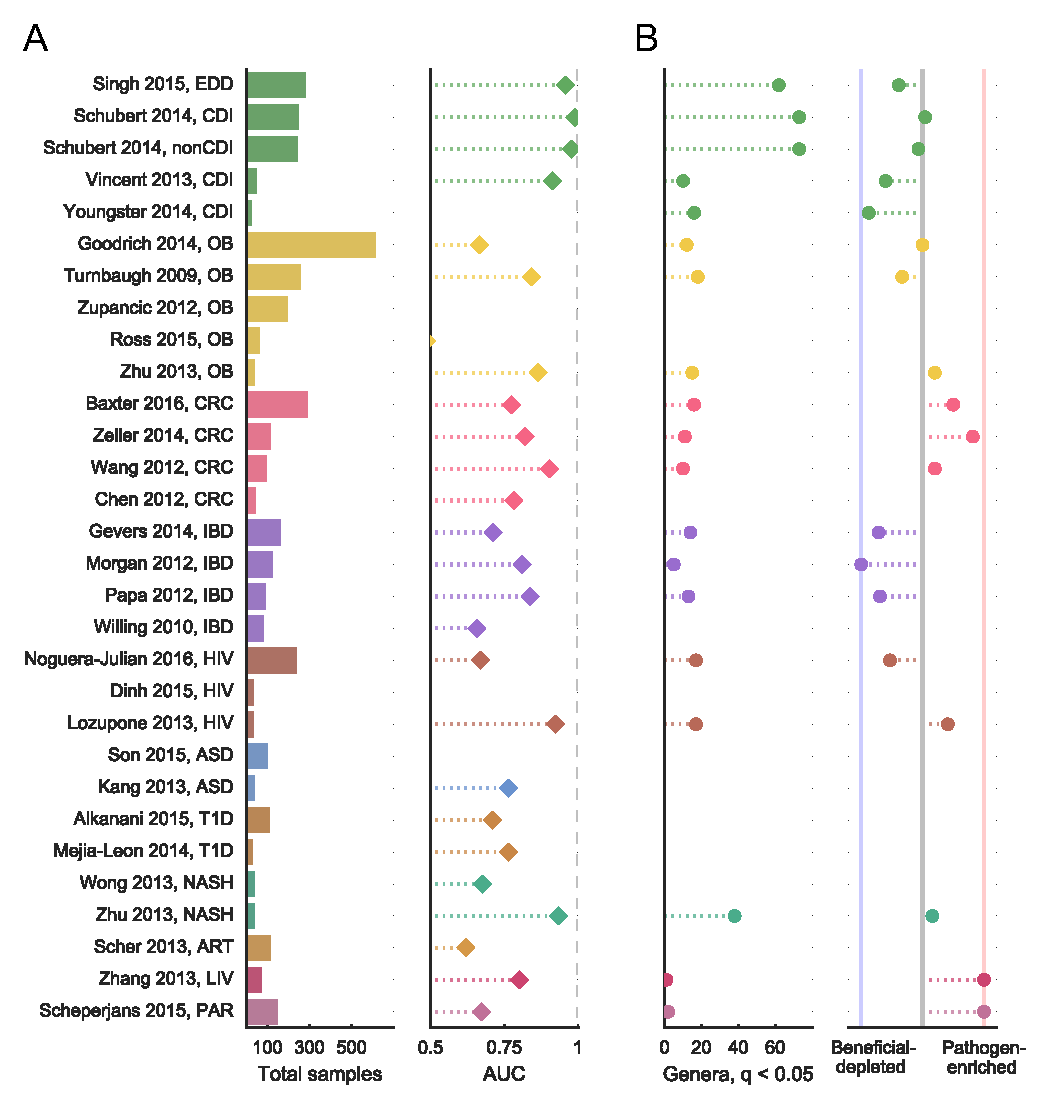
\includegraphics[width=1\textwidth]{samplesize_auc_nsig_balance.pdf}}
    \captionsetup{font=footnotesize,labelfont=footnotesize}
	\caption{\textbf{Most diseases show microbiome alterations, and consistent disease-associated shifts differ in their extent and direction.} (A) Left: Total sample size for each study included in these analyses. Additional information about each dataset can be found in Table \ref{tab:datasets}. Studies on the y-axis are grouped by disease and ordered by decreasing sample size (top to bottom). Right: Area under the ROC curve (AUC) for genus-level random forest classifiers. X-axis starts at 0.5, the expected value for a classifier which assigns labels randomly, and AUCs less than 0.5 are not shown. ROC curves for all datasets are in Supplementary Figure \ref{fig:roc_curves}. Note that Youngster et al. (2014) \cite{cdi-youngster} had only 4 distinct control patients was excluded from the Random Forest analysis. (B) Left: Number of genera with q $<$ 0.05 (Kruskal-Wallis (KW) test, Benjamini-Hochberg FDR correction) for each dataset. If a study has no significant associations, no point is shown. Right: Direction of the microbiome shift, i.e. the percent of total associated genera which were enriched in diseased patients. In datasets on the leftmost blue line, 100\% of associated (q $<$ 0.05, FDR KW test) genera are health-associated (i.e. depleted in patients relative to controls). In datasets on the rightmost red line, 100\% of associated (q $<$ 0.05, FDR KW test) genera are disease-associated (i.e. enriched in patients relative to controls). Supplementary Figures \ref{fig:overall_heatmap_qvalues} and \ref{fig:overall_heatmap_foldchange} show q-values and effects for each genus in each study.}
	\label{fig:fig1}
	\end{center}
\end{figure}

\newpage
\begin{figure}[h]
	\begin{center}
  	\makebox[\textwidth][c]{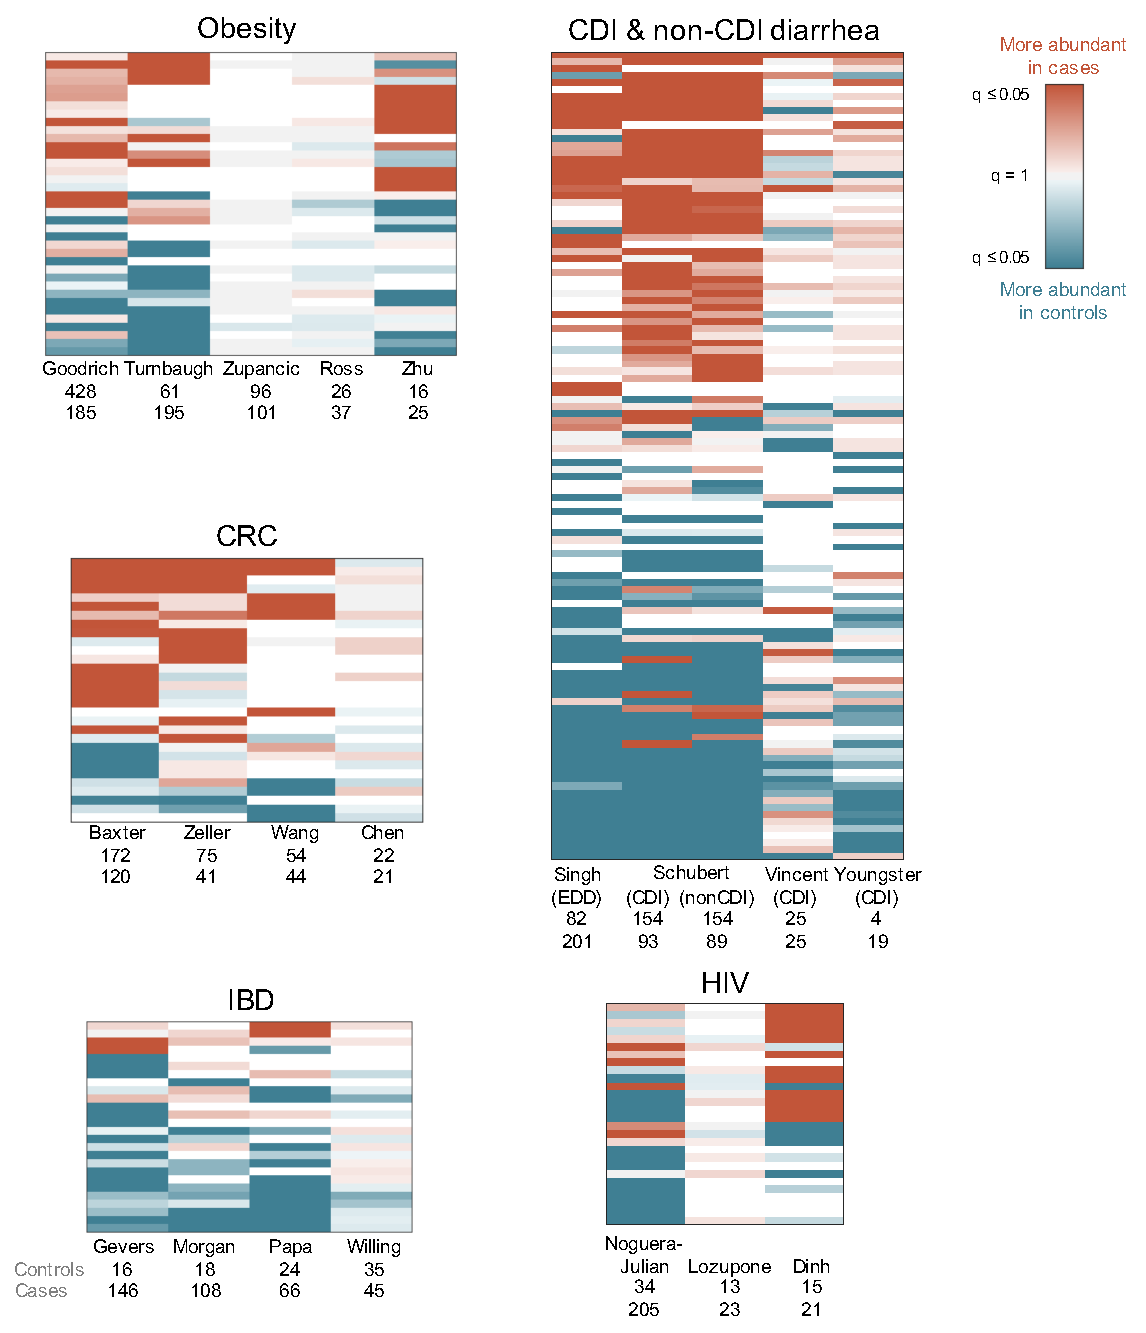
\includegraphics[width=0.9\textwidth]{disease_specific_heatmaps.pdf}}
    \captionsetup{font=footnotesize,labelfont=footnotesize}
	\caption{\textbf{Comparing results from multiple studies of the same disease reveals patterns in disease-associated microbiome alterations.} Heatmaps showing log10(q-values) for each disease (Kruskal-Wallis (KW) test, Benjamini-Hochberg FDR correction). Rows include all genera which were significant in at least one dataset within each disease, columns are datasets. Q-values are colored by direction of the effect, where red indicates higher mean abundance in disease patients and blue indicates higher mean abundance in controls. Opacity ranges from q = 0.05 to 1, where q values less than 0.05 are the most opaque and q values close to 1 are gray. White indicates that the genus was not present in that dataset. Within each heatmap, rows are ordered from most disease-associated (top) to most health-associated (bottom) (i.e. by the sum across rows of the log10(q-values), signed according to directionality of the effect). The extent of a disease-associated microbiome shift can be visualized by the number of rows in each disease heatmap; the directionality of a shift can be seen in the ratio of red rows to blue rows within each disease. See Supplementary Figure \ref{fig:supp_dis_specific} for genus (row) labels.}
	\label{fig:fig2}
	\end{center}
\end{figure}

\newpage
\begin{figure}[h]
	\begin{center}
  	\makebox[\textwidth][c]{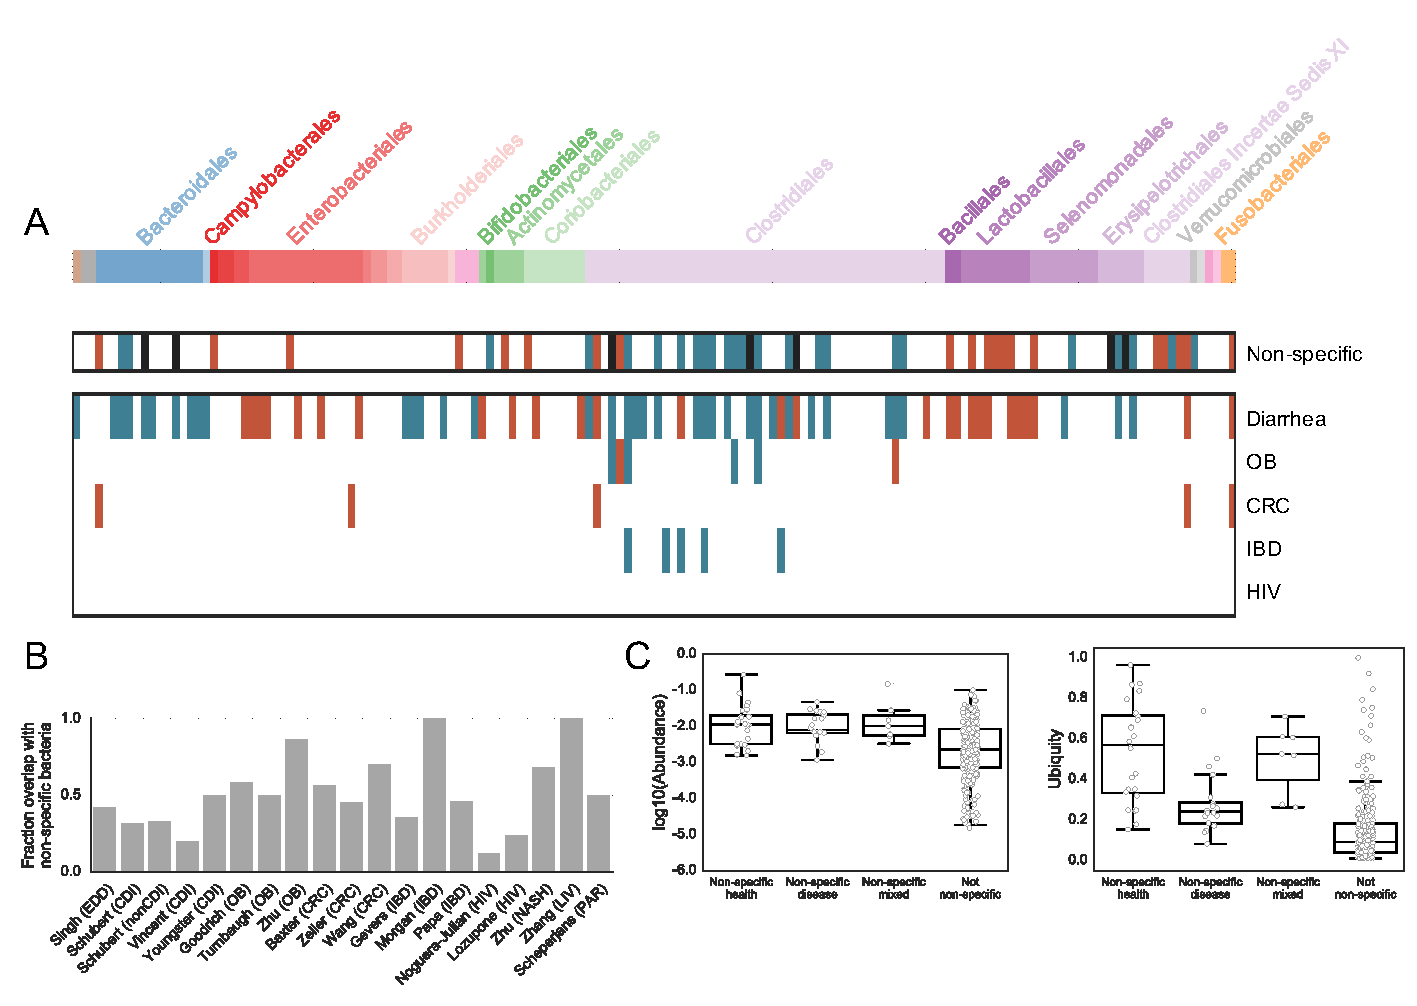
\includegraphics[width=\textwidth]{core_response.pdf}}
	\caption{\textbf{The majority of disease-associated microbiome alterations overlap with a non-specific microbial response to disease.} (A) Non-specific and disease-associated genera. Genera are in columns, arranged phylogenetically according to a PhyloT tree built from genus-level NCBI IDs (\url{http://phylot.biobyte.de}). Non-specific genera are associated with health (or disease) in at least two different \textit{diseases} (q $<$ 0.05, Kruskal-Wallis (KW) test, Benjamini-Hochberg FDR correction). Disease-specific genera are significant in the same direction in at least two \textit{studies} of the same disease (q $<$ 0.05, FDR KW test). As in Figure \ref{fig:fig2}, blue indicates higher mean abundance in controls and red indicates higher mean abundance in patients. Black bars indicate mixed genera which were associated with health in two diseases and also associated with disease in two diseases. Disease-specific genera are shown for diseases with at least 3 studies. Phyla, left to right: Euryarchaeota (brown), Verrucomicrobia Subdivision 5 (gray), Candidatus Saccharibacteria (gray), Bacteroidetes (blue), Proteobacteria (red), Synergistetes (pink), Actinobacteria (green), Firmicutes (purple), Verrucomicrobia (gray), Lentisphaerae (pink), Fusobacteria (orange). See Supplementary Figure \ref{fig:supp_meta_heatmap} for genus labels. (B) The percent of each study's genus-level associations which overlap with the shared response  (q $<$ 0.05, FDR KW test). Only datasets with at least one significant association are shown. (C) Overall abundance and ubiquity of non-specific genera across all patients in all datasets. Non-specific genera on the x-axis are as defined above.}
	\label{fig:fig3}
	\end{center}
\end{figure}

\bibliographystyle{unsrt}
\bibliography{meta-analysis/refs}


%% This is an example first chapter.  You should put chapter/appendix that you
%% write into a separate file, and add a line \include{yourfilename} to
%% main.tex, where `yourfilename.tex' is the name of the chapter/appendix file.
%% You can process specific files by typing their names in at the
%% \files=
%% prompt when you run the file main.tex through LaTeX.

\chapter{Framework for rational donor selection in fecal microbiota transplant clinical trials}

The contents of this chapter were submitted with
Claire Duvallet, Caroline Zellmer, Pratik Panchal, Shrish Budree, Majdi Osman, and Eric J. Alm as authors.

The supplementary information is in Appendix B.
The supplementary tables are at the end of the chapter.

\includepdf[pages=-, pagecommand={\thispagestyle{plain}}, scale=0.95]{fmt/ms}

%% This is an example first chapter.  You should put chapter/appendix that you
%% write into a separate file, and add a line \include{yourfilename} to
%% main.tex, where `yourfilename.tex' is the name of the chapter/appendix file.
%% You can process specific files by typing their names in at the
%% \files=
%% prompt when you run the file main.tex through LaTeX.
\chapter{Conclusions}

\section{Limitations and extensions of reported work}

In this thesis, I present three projects which overcome a variety of challenges to mine human microbiome data to extract clinical insights.
In the first project, I overcome the difficulty of identifying consistent biomarkers across highly variable lung and stomach communities by instead looking at the relationships between aerodigestive body sites within individual patients.
In the second project, I re-analyze gut microbiome datasets across many diseases and individual studies to identify consistent associations despite the technical challenges involved in extracting generalizable knowledge from the existing corpus of published studies.
In the third project, I present a framework to categorize disease-specific insights gleaned from previously performed analyses and experiments and leverage them to improve fecal microbiota transplant clinical trials.
Although performed in different contexts and with different goals in mind, these three computational projects share similar limitations.

First, the findings in each project suggest associations but do not and cannot confirm causal relationships.
In Chapter 2, although I demonstrate that the interpretation of the aspiration-associated perturbation is consistent across a variety of analyses and metrics, such associations would still need to be recapitulated and confirmed in an independent patient cohort before being further developed as a clinical diagnostic.
Also, many more mechanistic experiments and longitudinal retrospective cohort analyses would need to be done to confirm their association with aspiration-related respiratory infections and discover mechanistic explanations.
In Chapter 3, the consistent associations that I identify across many different gut microbiome studies and microbiome-related diseases can make no claim of causality: in all case-control microbiome datasets, it is not possible to determine whether the microbiome shifts are a cause of the disease or simply responding to the host's physiological state.
In fact, finding many non-specific disease- and health-associated bacteria across these datasets suggests that a large part of these associations are more likely to be responses to the host's general health status rather than specifically causal to any given disease.
To truly find disease-associated bacteria, researchers need to identify consistent associations across multiple cohorts of their disease of interest and ensure that these associations are specific to that disease, and perhaps even isolate the strains of interest to test their causality in animal models.
Finally, the conceptual framework that I present in Chapter 4 suggests one way to advance translational microbiome science but will need to be applied in many FMT trials before its impact on FMT trial successes can be confirmed.

A second limitation comes from the fact that these projects are anchored in the analysis of 16S rRNA data, which is more accessible than many 'omics data types but comes with its own set of inherent limitations.
16S data provides a window into which bacteria are present in microbial communities but does not indicate what functions these bacteria are performing.
Because disease-mediating effects will result from bacterial function, future work should strive to incorporate function into their studies, for example by analyzing metagenomics, metabolomics or transcriptomics data, or a combination of these data types.
I hope that as datasets become more readily available,  someone will perform a similar cross-disease meta-analysis as in Chapter 3, but instead based on metagenomics data.
I expect that a function-focused meta-analysis will find much more consistent and readily interpretable associations within studies of the same disease as well as across diseases.
Another limitation of 16S data is that in most cases it cannot resolve bacteria at the strain level.
Given that different strains of the same species have dramatically different clinical presentations, this is a crucial limitation in extracting clinically relevant associations from 16S microbiome data.
Strain-level resolution will be especially important in evaluating rational donor selection methods, where engraftment of specific donor strains may be an important factor mediating patient responses to FMT.

Finally, these studies are limited by their sample sizes.
Although the aerodigestive cohort presented in Chapter 2 and the meta-analysis in Chapter 3 are the largest of their kind to date, the analyses that I could perform were still limited by insufficient sample sizes.
In Chapter 2, I was unable to draw robust conclusions about the relationship between reflux and the aerodigestive microbiome because the number of patients with the respective samples and metadata was too small to sufficiently power my analysis.
In fact, throughout this project I frequently found my analyses limited by the necessary confluence of samples and metadata.
For example, I would have liked to analyze the combinatorial effects of proton pump inhibitors, aspiration, and reflux on the aerodigestive microbiome, but I simply did not have enough patients with the respective samples and metadata to perform any reasonably powered analyses.
The meta-analysis presented in Chapter 3 was also limited by the number of datasets and diseases.
Originally, I had hoped to compare disease-associated microbiome shifts in an unsupervised manner to identify patterns of shifts common to similar types of diseases.
For example, I wondered if I could find a consistent group of bacteria associated with inflammation across multiple inflammatory diseases.
However, I had a surprisingly difficult time finding datasets with publicly available raw data and associated patient-level clinical metadata, even given the large corpus of relevant published papers.
Thus, I did not acquire a large enough variety of diseases and datasets to enable this broader categorization of diseases and perform statistically meaningful analyses on these groups of datasets.
Finally, one of the main conclusions of the framework presented in Chapter 4 is that the usual sample sizes in FMT studies will almost always limit the power of retrospective analyses to identify key bacteria.
Because these studies are performed with human samples and sometimes require careful ethical justifications and considerable patient recruitment efforts, this challenge of small sample sizes is likely to remain an important limitation for future studies throughout the microbiome field.

\section{Re-analyzing existing datasets and data availability}

A core theme that has emerged from my thesis work is that re-analyzing existing microbiome datasets can add substantial value to our field.
One of my personal conclusions from the meta-analysis is that cross-sectional gut microbiome studies should be regularly contextualized within the existing published body of work.
Now that microbiome datasets are more readily available and bioinformatics tools to process and analyze them are becoming very accessible, I hope that researchers make it a habit to ask: are these associations consistent with ones from independent patient cohorts? Are they specific to my disease of interest or are they part of a non-specific response to health and disease?

I also found the value-add of re-analyzing datasets especially relevant in microbiome research led by clinicians.
For example, the original IBD FMT trials that I re-analyzed in Chapter 4 did not thoroughly investigate potential donor effects on patient response in their original studies.
This is expected in part because heterogenous donor response was not usually their primary question of interest, and also because their trials were not powered for these analyses.
However, now that multiple IBD FMT trials have been published with patient and donor microbiome sequencing data, hypotheses about what leads to improved patient response could be tested \textit{in silico}, as we did for butyrate producer abundance in Chapter 4.
In Chapter 3, many of my datasets were pulled from studies led by clinical researchers who may not have had access to the bioinformatics and statistical expertise to fully interrogate disease associations within their datasets.
By making their data publicly available, their work continued to contribute new knowledge to the field.
% maybe: Finally, re-analyzing published datasets adds value at little extra cost: recruiting patients, collecting samples, and generating data

Moving forward, I hope and expect that researchers continue to make their raw data publicly available and that re-analyses of such data become standard in the field.
Publicly available raw data allows researchers to ask and answer new questions, testing their hypotheses \textit{in silico} without the need for costly new studies.
New studies can also compare their results with existing work to determine which of their findings hold across different studies and which are specific to their specific study.
However, using published data in new contexts comes with challenges.
Batch effects, which result from different experimental and sequencing methods, can make it very difficult to compare data across different labs.
As a follow-up to the meta-analysis, I contributed to a method to correct for batch effects in case-control studies \cite{gibbons-2018}, and I hope that batch-correction methods keep being developed for this data type.
Another major challenge is data availability, and specifically clinical metadata like patient disease diagnosis.
Through this work, I have come to realize that raw data without its associated metadata is in almost all cases useless.
Given these challenges, standards for sharing data which respect patient privacy, clinicians' efforts for patient recruitment, and the needs of computational biologists will need to be agreed upon and upheld as a community.

\section{Partnerships between clinicians and computational biologists}

Throughout this thesis, I also came to appreciate the unique contributions that come from close partnerships between clinicians and computational biologists.
None of the projects in this thesis would have been possible without crucial contributions from our clinical counterparts.
Chapter 2 was only possible because our clinical PI, Rachel Rosen, identified and framed the questions of interest in this cohort so that I could then translate them into computational analyses that could provide answers with our data.
Working together in this way, we discovered new science and found clinically exciting results.
The meta-analysis in Chapter 3 was also significantly strengthened by the inclusion of datasets which were originally purely clinical investigations, and the framework presented in Chapter 4 was only possible because of our lab's strong ties with the clinical experts at OpenBiome.
I hope that the future of translational microbiome research establishes structures that encourage such close collaborations.
Systems to share raw data should be designed with these collaborations in mind: the process to deposit data should be accessible to clinicians, patient information should be protected while also providing easy access to analyses that don't use the protected information, and the metadata should be curated well enough to enable straightforward analyses without much manual curation but also flexible enough to allow for the variety of study designs pursued by clinicians.

\section{Finding knowledge in information}

A turning point in my thesis came when I read the 1976 paper coining the term "meta-analysis" \cite{glass-1976}.
In it, Glass argues for the importance and underappreciated value of consolidating and synthesizing information into knowledge, prizing work that aims to find meaning and draw conclusions from existing studies.
This was a turning point for two reasons.
First, it was the moment I became truly proud of my work, especially the meta-analysis: I realized that it was not just some sort of microbiome "stamp collection" endeavor that anyone with basic knowledge of computational tools could do, but was instead difficult and valuable work that I uniquely contributed to.
Second, it helped me recognize a uniting theme in all of my work as exactly what Glass wrote, "find[ing] the knowledge in the information."
I realized that in each analysis in this thesis, I aimed to move beyond statistical associations all the way to clinical implications.
I hope that as we move forward in this exciting and vibrant field, we collectively become less satisfied with simply reporting new information and emphasize instead efforts to synthesize existing knowledge and generate new insights that lead more directly to clinical impact.

\begin{singlespace}
\bibliography{chap1}
\bibliographystyle{unsrt}
\end{singlespace}

\appendix
\chapter{Supplementary Information for Chapter 2}

\input{aspiration/plosone_aspiratin_supplement.tex}

\chapter{Supplementary Information for Chapter 4}

\graphicspath{{meta-analysis/figures/}}

\section{Supplementary Notes}

\subsection{Re-processing and re-analyzing raw data yields results which are generally consistent with previously published results}\label{sec:lit_comp}

Our re-analyses of the 29 studies were largely consistent with the originally reported results, with the same taxonomic groups showing similar trends despite differences in data-processing methodologies.
We usually found fewer significant (q $<$ 0.05) differences between control and diseased groups, which is likely due to our choice of a non-parametric statistical test (Kruskall-Wallis) paired with a multi-test correction (FDR).
Thus, our results are more conservative.
We also collapsed to genus level in order to compare results across disparate studies, which prevented us from identifying species- or strain-specific associations which the original authors may have identified.
A major advantage of our re-analysis is that each data set was processed and analyzed in the same way, which allowed us to more directly compare results across studies and diseases.

\subsubsection{\textit{Clostridium difficile} Infection and enteric diarrhea are characterized by large-scale shifts in the microbiome (CDI; 4 studies)}

Schubert et al. (2014) looked at how the gut microbiota differed between CDI patients with diarrhea (n $=$ 94), non-CDI patients with diarrhea (n $=$ 89), and non-diarrheal controls (n $=$ 155) \cite{cdi-schubert}.
Similar to other CDI studies, the authors found a significant reduction in alpha diversity in patients with diarrhea (Dunn’s multiple-comparison test on AMOVA, p $<$ 0.0001).
They found that OTUs from the \textit{Ruminococcaceae}, \textit{Lachnospiraceae}, \textit{Bacteroides}, \textit{Prevotellaceae}, and \textit{Porphyromonadaceae} families were enriched in healthy subjects relative to patients with CDI and non-CDI diarrhea.
They also showed that OTUs from the \textit{Enterococcus} genus and the \textit{Enterobacteriaceae} and \textit{Erysipelotrichaceae} families were more prevalent in patients with diarrhea.
In our analysis of the data, we also observed a significant reduction in alpha diversity in patients with diarrhea (q $<=$ 0.05, KW test).
Similarly, we found that \textit{Enterobacteriaceae}, \textit{Enterococcus}, and \textit{Erysipelotrichaceae} were enriched in CDI patients, in addition to \textit{Fusobacterium}, \textit{Parvimonas}, \textit{Veillonella}, \textit{Carnobacterium}, \textit{Streptococcus}, \textit{Tetragenococcus}, \textit{Lactobacillus}, \textit{Pediococcus}, \textit{Gemella}, \textit{Staphylococcus}, \textit{Butyricicoccus}, \textit{Robinsoniella}, \textit{Clostridium XlVa}, \textit{Clostridium XlVb}, \textit{Ruminococcus2}, \textit{Flavonifractor}, \textit{Gemmiger}, \textit{Mogibacterium}, \textit{Peptostreptococcus}, \textit{Clostridium XI}, \textit{Eggerthella}, \textit{Atopobium}, \textit{Actinomyces}, \textit{Arthrobacter}, \textit{Aggregatibacter}, \textit{Pseudomonas}, and \textit{Dysgonomonas}.
As in the original study, we found that \textit{Bacteroides}, \textit{Alistipes}, \textit{Anaerovorax}, \textit{Oxalobacter}, \textit{Bordetella}, \textit{Prevotellaceae}, \textit{Porphyromonadaceae}, \textit{Lachnospiraceae}, and \textit{Ruminococcaceae} were more abundant in the healthy controls.
We also found \textit{Turicibacter}, \textit{Dialister}, \textit{Eubacterium}, \textit{Asteroleplasma}, \textit{Cloacibacillus}, \textit{Bordetella}, \textit{Oxalobacter}, \textit{Sutterella}, \textit{Parasutterella}, \textit{Desulfovibrio}, \textit{Sediminibacterium}, and \textit{Methanobrevibacter} to be enriched in the controls (q $<=$ 0.05, KW tests).
Overall, our analysis closely matched what was presented in the original manuscript.

Vincent et al. (2013) compared 25 patients with CDI to 25 healthy control patients \cite{cdi-vincent}.
The authors found a significant reduction in alpha diversity (p $<=$ 0.05, Mann-Whitney U test).
They also report a reduction in \textit{Bacteroidaceae} and \textit{Clostridiales Incertae Sedis XI} in CDI patients relative to controls, and an enrichment in \textit{Enterococcaceae} in CDI patients (p $<$ 0.05, logistic regression).
After reprocessing these data and collapsing abundances to the genus level, we observed a similar reduction in alpha diversity (q $<=$ 0.05, KW test). We saw that the \textit{Enterococcaceae} genera \textit{Enterococcus} and \textit{Proteus} were enriched in CDI patients. Healthy controls showed higher levels of \textit{Fusobacterium}, \textit{Peptoniphilus}, \textit{Murdochiella}, \textit{Anaerococcus}, \textit{Finegoldia}, \textit{Odoribacter}, \textit{Prevotella}, and \textit{Parabacteroides} relative to CDI patients. In summary, our results are fairly similar to the authors' original analysis, showing a depletion in \textit{Bacteroidetes} and an enrichment in \textit{Proteobacteria} in CDI patients.

Youngster et al. (2014) applied fecal microbiota transplants (FMTs) with materials collected from 5 healthy donors to 20 patients with recurrent \textit{Clostridium difficile} infections (CDIs) \cite{cdi-youngster}.
The goal of this study was to determine whether nasal-gastric tube or colonoscopy administration of FMTs was most effective for treating CDIs (i.e. half of the CDI patients received one or the other treatment).
The authors reported a significant reduction in alpha diversity in CDI patients vs. the healthy donors (p $<$ 0.001, Mann-Whitney test).
They did not assess whether there were significant differences in microbial community composition between CDI patients and donors, although they show that composition becomes more similar to donors following FMT.
In our analysis, we also found a significant reduction in alpha diversity (p $<=$ 0.05, KW test). \textit{Enterococcus} was enriched in CDI patients relative to healthy stool donors (q $<=$ 0.05, KW tests) and 15 genera were depleted in CDI patients relative to healthy controls.
Healthy donors were enriched in genera from \textit{Ruminococcaceae} and \textit{Lachnospiraceae} families, in addition to the genera \textit{Dialister} and \textit{Anaerosporobacter}.

Singh et al. (2015) examined differences in the gut microbiome between individuals with enteric infections (n=200) and healthy controls (n=75) \cite{edd-singh}.
The authors report a significant drop in alpha diversity in diseased patients relative to the controls (unknown test).
They also report a general reduction in the dominance of \textit{Firmicutes} and \textit{Bacteroidetes} phyla and an increase in the prevalence of \textit{Proteobacteria} in diseased patients.
Specifically, they report an increase in the abundance of \textit{Enterobacteriaceae}, \textit{Lactobacillaceae}, \textit{Pasteurellaceae}, \textit{Streptococcus}, \textit{Bacilli}, \textit{Escherichia},  \textit{Haemophilus}, and certain \textit{Ruminococcus} species in patients with diarrhea.
In healthy people, they report a significant enrichment in \textit{Verrucomicrobia}, \textit{Dorea}, \textit{Blautia}, \textit{Holdermania}, \textit{Ruminococcaceae}, \textit{Lachnospiraceae}, \textit{Butyricimonas}, \textit{Faecalibacterium}, \textit{Bacteroidaceae}, and \textit{Bifidobacterium}, \textit{Sutterella}, \textit{Parabacteroides}, \textit{Rikenellaceae}, and \textit{Oscillospira}.
After re-processing the data, we found very similar results to those originally reported.
We found that alpha diversity was significantly lower in patients with enteric infections (q $<=$ 0.05, KW test).
We saw significant enrichment in \textit{Proteobacteria} families in patients with diarrhea, including \textit{Enterobacteriaceae}, \textit{Pasteurellaceae}, \textit{Campylobacteraceae}, and \textit{Neisseriaceae}.
We also saw higher levels of \textit{Fusobacterium}, \textit{Parvimonas}, \textit{Veillonella}, \textit{Lactococcus}, \textit{Streptococcus}, \textit{Enterococcus}, \textit{Tetragenococcus}, \textit{Gemella}, \textit{Ruminococcus II}, \textit{Peptostreptococcus}, and \textit{Collinsella} in diseased patients.
In the healthy controls, we found enrichment of 43 genera, including \textit{Sutterella}, \textit{Verrucomicrobia} (\textit{Akkermansia}), \textit{Ruminococcaceae}, \textit{Lachnospiraceae}, \textit{Bacteroidaceae}, and \textit{Bifidobacterium}.
In addition, we saw higher levels of several members of \textit{Rumminococcaceae}, \textit{Lachnospiraceae}, and \textit{Bacteroidales} in healthy controls (q $<=$ 0.05, KW tests).
Overall, our results largely overlap with those presented, but we identify a number of significant taxa that were not originally reported.

Taken together, we see large-scale shifts in the microbiome associated with both CDI and non-CDI diarrhea.
The dysbiosis of enteric infection and diarrhea is quite consistent across studies.
In general, \textit{Proteobacteria} increase in prevalence in patients with diarrhea, with a concomitant decrease in \textit{Bacteroidetes} and \textit{Firmicutes}.
In particular, we see a reduction in butyrate-producing Clostridia, including genera within \textit{Ruminococcaceae} and \textit{Lachnospiraceae} families, which have been associated with a healthy gut.
We also see in increase in prevalence of organisms often associated with lower pH and higher oxygen levels of the upper-gut, like \textit{Lactobacillaceae} and \textit{Enterobacteriaceae} \cite{donaldson2016gut}, in patients with diarrhea.
Thus, diarrhea leads to consistent and large-scale rearrangements in the composition of the gut microbiome.

\subsubsection{Colorectal Cancer has a consistent, ootentially pathogenic microbial signature (CRC; 4 studies)}

Baxter et al. (2016) looked at differences in the microbiomes of 120 colorectal cancer (CRC) patients, 198 patients with non-cancerous adenomas, and 172 healthy controls \cite{crc-baxter}.
Similar to prior work, the authors found that \textit{Porphyromonas}, \textit{Peptostreptococcus}, \textit{Parvimonas}, and \textit{Fusobacterium} were positively associated with CRC (random forest classifiers).
Furthermore, they found that the absence of certain \textit{Lachnospiraceae} species was associated with the presence of adenomas.
We found similar patterns in our re-analysis of these data, with \textit{Fusobacterium}, \textit{Peptostreptococcus}, \textit{Parvimonas}, and \textit{Porphyromonas} enriched in CRC patients (q $<=$ 0.05, KW tests).
We also found higher levels of \textit{Victivallis}, \textit{Peptoniphilus}, \textit{Anaerococcus}, \textit{Catenibacterium}, \textit{Staphylococcus}, \textit{Collinsella}, \textit{Enterobacter}, and \textit{Alloprevotella} in CRC patients (q $<=$ 0.05, KW tests).
We found that healthy controls were enriched in \textit{Lachnobacterium} (genus within \textit{Lachnospiraceae}), \textit{Gemmiger} (within \textit{Rumminococcaceae}), \textit{Clostridium XVIII}, and \textit{Haemophilus} (q $<=$ 0.05, KW tests).
Overall, these results match what has been reported previously for CRC \cite{brennan2016gut}.

Zeller et al. (2014) collected microbiome data from 41 CRC patients and 75 control patients \cite{crc-zeller}.
At the phylum level, they found that \textit{Proteobacteria}, \textit{Fusobacteria}, and \textit{Bacteroidetes}, were more abundant in CRC patients, while \textit{Firmicutes} and \textit{Actinobacteria} were enriched in control patients.
At the genus level, the authors report higher levels of \textit{Fusobacterium}, \textit{Pseudoflavonifractor}, \textit{Peptostreptococcus}, \textit{Leptotrichia}, \textit{Porphyromonas}, \textit{Desulfovibrio}, \textit{Parvimonas}, \textit{Selenomonas}, and \textit{Bilophila} in CRC patients (q $<=$ 0.1, FDR-corrected Wilcoxon tests).
Healthy controls were enriched in \textit{Bifidobacterium}, \textit{Acinetobacter}, \textit{Campylobacter}, \textit{Ruminococcus}, and \textit{Eubacterium} genera (q $<=$ 0.1, FDR-corrected Wilcoxon tests).
In our re-analysis we found enrichment of \textit{Fusobacterium}, \textit{Parvimonas}, \textit{Flavonifractor}, \textit{Anaerotruncus}, \textit{Anaerovorax}, \textit{Peptostreptococcus}, \textit{Comamonas}, \textit{Eikenella}, \textit{Butyricimonas}, and \textit{Porphyromonas} genera in CRC patients (q $<=$ 0.05, KW tests).
In healthy patients, we found higher levels of \textit{Anaerostipes} (within \textit{Lachnospiraceae}; q $<=$ 0.05, KW tests).

Wang et al. (2011) analyzed a cohort of 46 CRC patients and 56 healthy controls \cite{crc-zhao}.
The authors found no difference in alpha diversity between CRC and control patients.
CRC patients had higher abundances of \textit{Porphyromonas}, \textit{Escherichia-Shigella}, \textit{Enterococcus}, \textit{Streptococcus}, and \textit{Peptostreptococcus} genera (p $<=$ 0.05, Mann-Whitney).
The authors report that healthy controls were enriched \textit{Bacteroides}, \textit{Roseburia}, \textit{Alistipes}, \textit{Eubacterium}, and \textit{Parasutterella} genera (p $<=$ 0.05, Mann-Whitney).
We found very similar results in our re-analysis of these data.
We saw greater levels of \textit{Enterococcus}, \textit{Peptostreptococcus}, \textit{Enterobacter}, \textit{Klebsiella}, \textit{Escherichia-Shigella}, and \textit{Porphyromonas} genera in CRC patients (q $<=$ 0.05, KW tests).
And we observed significantly higher levels of \textit{Bacteroides}, and several genera within \textit{Lachnospiraceae} in healthy controls (q $<=$ 0.05, KW tests).
Furthermore, we also did not detect any significant differences in alpha diversity between CRC and healthy patients.

Chen et al. (2012) analyzed stool from 22 healthy patients and 21 CRC patients \cite{crc-xiang}.
The authors found that \textit{Paraprevotella}, \textit{Eubacterium}, \textit{Desulfovibrio}, \textit{Mogibacterium}, \textit{Collinsella}, \textit{Anaerotruncus}, \textit{Slackia}, \textit{Anaerococcus}, \textit{Porphyromonas}, \textit{Fusobacterium}, and \textit{Peptostreptococcus} genera were significantly enriched in CRC patients relative to controls, while \textit{Bifidobacterium}, \textit{Faecalibacterium}, and \textit{Blautia} were reduced in CRC patients (p $<=$ 0.05, Mann-Whitney).
In our re-analysis of this data set, we found no significant differences between CRC and control patients.
Again, this is likely due to the small number of replicates and our implementation of multiple-test corrections.
However, non-significant trends were largely in agreement with the original results.

Across these four colorectal cancer studies, we find significant agreement.
Dysbiosis associated with CRC is generally characterized by increased prevalence of \textit{Fusobacterium}, \textit{Porphyromonas}, \textit{Peptostreptococcus}, \textit{Parvimonas}, \textit{Leptotrichia}, \textit{Desulfovibrio}, and \textit{Anaerococcus} genera (i.e. these genera were higher in CRC patients in 2 or more studies).
In addition, there is a consistent decrease in the abundances of \textit{Faecalibacterium}, \textit{Blautia}, \textit{Bacteroides} genera and organisms from the \textit{Lachnospiraceae} family in CRC patients.
CRC appears to have a smaller impact on overall community structure than diahrrea.
Indeed, we saw no significant differences in alpha diversity between healthy controls and CRC patients.
In summary, CRC is characterized by a consistent enrichment of disease-associated bacteria.

\subsubsection{Inflammatory Bowel Disease is characterized by a depletion of health-associated bacteria (IBD - Ulcerative Colitis and Crohn's Disease; 4 studies)}

Gevers et al. (2014) looked for microbial signatures of Crohn's disease (CD) samples across 447 CD patients and 221 non-IBD controls \cite{ibd-gevers}.
Non-IBD controls were patients with non-inflammatory conditions such as abdominal pain and diarrhea.
The authors report increased abundance of \textit{Enterobacteriaceae}, \textit{Pasteurellaceae}, \textit{Veillonellaceae}, and \textit{Fusobacteriaceae} in CD patients.
CD patients also showed a drop in the abundances of \textit{Erysipelotrichales}, \textit{Bacteroidales}, and \textit{Clostridiales} (\textit{Ruminococcaceae} and \textit{Lachnospiraceae}) taxa.
These results were based on a mixture of 16S amplicon and shotgun metagenomic sequencing.
In our re-analysis of the 16S stool data, we found significant enrichment in \textit{Anaerosporobacter}, \textit{Roseburia}, \textit{Hespellia}, \textit{Ruminococcus II}, \textit{Eubacterium}, \textit{Pseudoflavonifractor}, \textit{Sporobacter}, \textit{Ruminococcus}, \textit{Subdoligranulum}, \textit{Papillibacter}, \textit{Collinsella}, and \textit{Methanobrevibacter} in healthy patients (q $<=$ 0.05, KW tests).
The only genera that we saw significantly enriched in CD patients were \textit{Lactobacillus} and \textit{Acetanaerobacterium} (q $<=$ 0.05, KW tests).
We found a similar set of taxa enriched in the controls, but did not detect as many significant CD-enriched genera as the authors reported.
This is likely due to the fact that we restricted our analysis to the 16S stool data.
However, we saw non-significant trends in \textit{Enterobacteriaceae} and \textit{Veillonellaceae} consistent with the results reported in the original paper.

Morgan et al. (2012) studied a cohort of 119 CD patients, 74 UC patients, and 27 healthy controls \cite{ibd-hut}.
The authors found that healthy patients’ gut microbiomes were significantly enriched in \textit{Roseburia}, \textit{Phascolarctobacterium}, and an unclassified genus in the family \textit{Veillonellaceae} (multivariate linear model, q $<=$ 0.25).
Patients with UC showed significantly higher levels of \textit{Clostridiaceae} (multivariate linear model, q $<=$ 0.25).
In our re-analysis, we did not find any genera that were significantly enriched in IBD patients.
We found that healthy patients had significantly greater abundances of \textit{Ruminococcus}, and \textit{Gemmiger} relative to both UC and CD patients (q $<=$ 0.05, KW tests).
Additionally, CD patients were depleted in \textit{Clostridium IV} relative to healthy controls (q $<=$ 0.05, KW tests).

Papa et al. (2012) studied a cohort of 23 CD patients, 43 UC patients, and 24 non-IBD controls \cite{ibd-papa}.
Non-IBD controls were patients with symptoms such as: constipation, abdominal pain, gastroesophageal reflux, poor weight gain, diarrhea, blood in stool and oropharyngeal dysphagia.
At the genus level, they found that controls were enriched in \textit{Alistipes}, \textit{Subdoligranulum}, \textit{Anaerovorax}, \textit{Oscillibacter}, \textit{Parabacteroides}, \textit{Odoribacter}, \textit{Ruminococcus}, \textit{Butyricicoccus}, \textit{Akkermansia}, \textit{Anaerotruncus}, \textit{Sporobacter}, \textit{Phascolarctobacterium}, \textit{Lawsonia}, \textit{Ethanoligenens}, \textit{Peptococcus} relative to IBD patients (KW, q $<$ 0.01).
The only genus that was found to be enriched in IBD patients was \textit{Escherichia-Shigella}.
In our re-analysis, we also found \textit{Escherichia-Shigella} and \textit{Cronobacter} to be enriched in patients with IBD (q $<=$ 0.05, KW tests).
When comparing healthy controls with UC patients, we also found an enrichment of \textit{Haemophilus} in the UC patients.
Control patients showed higher abundances of \textit{Phascolarctobacterium}, \textit{Butyricicoccus}, \textit{Ruminococcus II}, \textit{Oscillibacter}, \textit{Ruminococcus}, \textit{Gemmiger}, \textit{Subdoligranulum}, \textit{Clostridium IV}, \textit{Odoribacter}, \textit{Alistipes}, and \textit{Parabacteroides} relative to all IBD patients (q $<=$ 0.05, KW tests).
Additionally, control patients were enriched in \textit{Clostridium XIVa}, \textit{Flavonifractor}, and \textit{Akkermansia} relative to UC patients.
Overall, our results match very closely what was found in the original paper.

Willing et al. (2010) compared 29 CD patients and 16 UC patients to 35 healthy controls \cite{ibd-engstrand}.
The authors reported variable, and sometimes opposing shifts in the microbiomes of patients with UC, ileal CD and colonic CD at different taxonomic resolutions.
We found no significant differences between IBD and healthy patients in our re-analysis.
When comparing healthy controls with CD cases only, we found an enrichment of \textit{Butyricicoccus} and \textit{Oscillibacter} in the control patients (q $<=$ 0.05, KW tests).

In summary, there are certain consistencies across IBD studies.
IBD patients tend to be depleted in butyrate-producing clostridia: \textit{Ruminococcus} and \textit{Lachnospiraceae}.
The organisms the are enriched in CD and UC patients tend to vary across studies.
One consistency is organisms associated with the upper gut, like \textit{Lactobacillus} and \textit{Enterobacteriaceae} appear to be enriched in IBD patients \cite{donaldson2016gut}.
This result fits with the reduced stool transit times associated with IBD (i.e. diarrhea).

\subsubsection{Obesity shows a somewhat inconsistent microbial signature (OB; 5 studies)}

Goodrich et al. (2014) studied a cohort of 416 twin pairs: 422 normal BMI, 322 overweight, and 185 obese \cite{ob-goodrich}.
The authors report higher levels of \textit{Lactobacillaceae}, \textit{Eggerthella}, and \textit{Lachnospiraceae} (\textit{Blautia} and \textit{Dorea}) in obese individuals (q $<$ 0.05, FDR-corrected T-test).
They showed enrichment for \textit{Christensenellaceae}, \textit{Dehalobacterium}, \textit{Lachnospira}, \textit{Mogibacteriaceae}, \textit{Rikenellaceae}, \textit{Methanobre}, \textit{Coriobacteriaceae}, \textit{Peptococcaceae}, \textit{Oscillospira}, \textit{Ruminococcaceae}, and \textit{Sarcina} in healthy BMI individuals (q $<$ 0.05, FDR-corrected T-test).
In our re-analysis, we found higher levels of \textit{Streptococcus}, \textit{Weissella}, \textit{Roseburia}, \textit{Blautia}, \textit{Clostridium XlVb}, and \textit{Mogibacterium} in obese individuals, while \textit{Robinsoniella}, \textit{Ruminococcaceae} (\textit{Oscillibacter}, \textit{Pseudoflavonifractor}, \textit{Sporobacter}, and \textit{Anaerofilum}), and \textit{Anaerovorax} were more abundant in low-BMI individuals (q $<=$ 0.05, KW tests).
Our results only partially agree with the authors' original findings, which may be due to the fact that we used a different statistical test and OTU-calling method and that we binned the data at the genus level.

Zupancic et al. (2012) analyzed 310 individuals from an Amish population with varying BMIs \cite{ob-zupancic}.
They found a significant positive correlation between the abundance of \textit{Collinsella} and BMI (i.e. enriched in obese individuals), while \textit{Lachnobacterium}, \textit{Anaerotruncus}, \textit{Faecalibacterium}, and \textit{Clostridium} were negatively correlated with BMI (i.e. enriched lean individuals) (p < 0.001, Spearman correlation).
We found no significant differences in the proportion of genera between lean and obese individuals in our re-analysis.

Turnbaugh et al. (2008) looked differences in gut microbial community structure between 31 monozygotic and 23 dizygotic twin pairs concordant for leanness or obesity \cite{ob-gordon}.
The authors report a reduction in alpha diversity in obese individuals.
They also report a significant decrease in \textit{Bacteroidetes}  and an increase in \textit{Actinobacteria} in obese twins.
In our re-analysis of these data, we did not see a significant reduction in alpha diversity (Supplementary Figure \ref{fig:fig_alpha}).
We found significant increases in \textit{Catenibacterium}, \textit{Acidaminococcus}, \textit{Megasphaera}, \textit{Lactobacillus}, \textit{Roseburia}, and \textit{Collinsella} in obese twins (q $<=$ 0.05, KW tests).
\textit{Coprobacillus}, \textit{Clostridium XVIII}, \textit{Phascolarctobacterium}, \textit{Clostridium XlVb}, \textit{Oscillibacter}, \textit{Flavonifractor}, \textit{Pseudoflavonifractor}, \textit{Ruminococcus}, \textit{Clostridium IV}, \textit{Gordonibacter}, \textit{Alistipes}, and \textit{Barnesiella} were significantly enriched in lean twins (q $<=$ 0.05, KW tests).

Ross et al. (2015) looked at 63 Mexican American patients with varying BMIs \cite{ob-ross}.
They found no significant differences between patients with high and low BMIs within their 63 patient cohort, but identified several significant differences between their patient population and the HMP data set.
However, it is unclear whether these differences were related to obesity, so we do not discuss them here.
Our re-analysis of these results also found no significant differences in the relative abundances of bacterial genera between high- and low-BMI subjects.

Zhu et al. (2013) compared across a cohort of 16 healthy and 25 obese patients, in addition to 22 patients with Nonalcoholic steatohepatitis (see below) \cite{nash-baker}.
For obesity, the authors found that \textit{Prevotella} was enriched in high-BMI patients, while healthy controls showed significantly greater relative abundances of \textit{Bifidobacterium}, \textit{Blautia}, and \textit{Faecalibacterium} (p $<=$ 0.05, ANOVA with post-hoc Tukey's tests).
In our re-analysis of these data, we found a significant enrichment of \textit{Peptoniphilus}, \textit{Anaerococcus}, \textit{Finegoldia}, \textit{Leuconostoc}, \textit{Mogibacterium}, \textit{Varibaculum}, \textit{Campylobacter}, \textit{Prevotella}, and \textit{Porphyromonas} in obese patients (q $<=$ 0.05). Healthy patients were significantly enriched in \textit{Akkermansia}, \textit{Murdochiella}, \textit{Blautia}, \textit{Lachnospiracea incertae sedis}, and \textit{Clostridium IV}, \textit{Anaerovorax} (q $<=$ 0.05, KW tests).

Overall, we found several differences between lean and obese patients that were consistent across at least two studies.
\textit{Roseburia} and \textit{Mogibacterium} were enriched in obese individuals in more than one study. \textit{Pseudoflavonifractor}, \textit{Oscillobacter}, \textit{Anaerovorax} and \textit{Clostridium IV} were enriched in the controls across more than one study. However, no genera showed consistent differences across three or more studies.
Our results are largely consistent with a recent meta-analysis of obesity studies, which found no universal signature of human obesity \cite{Sze07092016}.

\subsubsection{Human Immunodeficiency Virus microbial signature is confounded with patient cohorts (HIV; 3 studies)}

Dinh et al. (2015) compared the gut microbiome from 16 healthy patients to 22 patients with chronic HIV infections \cite{hiv-dinh}.
The authors report an general enrichment in \textit{Proteobacteria} in HIV-infected patients.
At the genus level, they found a significant enrichment in \textit{Barnesiella} and a depletion in \textit{Alistipes} in HIV-infected patients (LEfSe, p $<$ 0.05).
In our re-analysis of these data we found no significant differences in the relative abundances of genera between healthy and HIV-infected patients.

Lozupone et al. (2013) looked at 22 HIV-positive patients and 13 healthy controls \cite{lozupone2013alterations}.
The authors reported enrichment of \textit{Prevotella}, \textit{Catenibacterium}, \textit{Dialister}, \textit{Allisonella}, and \textit{Megasphera} genera in HIV-positive patients, while \textit{Bacteroides} and \textit{Alistipes} were more abundant in controls (p $<$ 0.05, ANOVA).
We found all the associations reported above in our re-analysis.
Additionally, we saw higher relative abundances of \textit{Erysipelotrichaceae incertae sedis}, \textit{Peptococcus}, \textit{Mogibacterium}, \textit{Peptostreptococcus}, \textit{Desulfovibrio}, \textit{Hallella}, and \textit{Alloprevotella} in HIV-positive patients.
And healthy patients were also enriched in \textit{Oridibacter}, \textit{Anaerostipes}, and \textit{Parasutterella}.
Many of the significant genera from the Lozupone study were shown to be strongly associated with sexual behavior in the Noguera-Julian study (i.e. these genera were significantly different in men who have sex with men versus other subjects; see below) and may not necessarily be related to HIV status.

Noguera-Julian et al. (2016) studied a cohort of 293 HIV-infected patients and 57 healthy controls.
The authors found that many putative associations between HIV and the microbiome were driven by sexual preference (i.e. \textit{Prevotella}, along with several other genera, were enriched in men who have sex with men (MSM)).
After controlling for this demographic confounder, the authors reported that they were not able to classify HIV positive and negative patients MSM patients.
Due to the large size of their study, the authors were able to separate the influences of sexual behavior and HIV-status from one another and found that the majority of reported HIV-associations are likely confounded with sexual behavior.

Overall, there is not yet a strong consensus on the impacts of HIV on the human gut microbiome.
Differences between patient cohorts may have obscured any putative HIV signal across studies.
For example, all the patients in the Dinh et al. (2015) study were on antiretroviral therapy (ART), while only some of the patients in the other two studies were on ART.
Noguera-Julian et al. (2016) found that patients who initiated ART within the first 6 months of HIV infection were able to maintain gut microbial community richness, unlike patients that were not on ART.
In addition, the Noguera-Julian et al. (2016) paper was able to show that prior results showing enrichment of \textit{Prevotella} in HIV-positive patients was an artifact due to this genera being enriched in men who have sex with men.

\subsubsection{Autism Spectrum Disorder (ASD; 2 studies)}

Kang et al. (2013) reported a reduced prevalence of \textit{Prevotella} and other fermentative organisms in the guts of ASD children \cite{asd-kb}.
In particular, the authors showed significant (q $<=$ 0.05, Mann-Whitney) depletion in unclassified \textit{Prevotella} and \textit{Veillonellaceae} genera in autistic children (n $=$ 20 treatment and 20 controls).
The authors also note a reduced alpha diversity in autistic children.
After reprocessing these data, we found no significant differences in alpha diversity or genera abundances between autistic and control children (Figure 1; q $>$ 0.05, Kruskal-Wallis).
The original conclusion that \textit{Prevotella} and \textit{Veillonellaceae} were different was based on q-values of 0.04, which is only moderately convincing evidence against the null-hypothesis.
Therefore, the loss of this marginal significance (for q $<=$ 0.05) is unsurprising when using a different statistical test.

In a more recent study, Son et al. (2015) found no significant differences in microbial community diversity or composition between autistic and neurotypical children (n $=$ 59 ASD and 44 neurotypical) \cite{asd-son}.
One genus, representing chloroplast sequences, was associated with ASD children with functional constipation, but this signal appeared to be due to dietary intake of chia seeds.
Similar to the authors’ findings, we did not detect any significant differences in genera abundances between ASD children and neurotypical children in the reprocessed data (q $>$ 0.05, Kruskal-Wallis).

Taken together, we find no evidence for changes in the composition or diversity of the gut microbiome in response to ASD.
However, we cannot discount subtle dysbiosis (i.e. small effect size) in response to ASD due to the small number of patients in each study.

\subsubsection{Type 1 Diabetes (T1D; 2 studies)}

Alkanani et al. (2015) compared 23 healthy patients to 35 early-onset T1D patients and 21 seropositive T1D patients \cite{t1d-alkanani}.
The authors report higher relative abundances of \textit{Lactobacillus}, \textit{Prevotella} and \textit{Staphylococcus} genera in healthy patients (p $<$ 0.05, Wilcoxon).
T1D patients showed higher levels of \textit{Bacteroides} (p $<$ 0.05, Wilcoxon).
In our re-analysis, we found no significant differences in bacterial genera across healthy and diseased patients.

Mejia-Leon et al. (2014) compared 8 healthy patients to 8 early-onset T1D patients and 13 T1D patients who had received 2 years of treatment \cite{t1d-mejia}.
Similar to Alkanani et al. (2015), they found controls to be significantly enriched in \textit{Prevotella} and T1D patients enriched in \textit{Bacteroides} (p $<$ 0.05, ANOVA, Tukey-Kramer test).
They also found higher levels of \textit{Acidaminococcus} and \textit{Megamonas} genera (in the \textit{Veillonellaceae} family) in the controls (p $<$ 0.05, ANOVA, Tukey-Kramer test).
We saw no significant differences in our re-analysis of these data.

Overall, the original authors report a consistent increase in \textit{Bacteroides} and depletion in \textit{Prevotella} genera associated with T1D.
However, our re-analysis found that these differences did not pass our significance threshold.
Thus, we cannot yet conclude that there is a consistent dysbiosis associated with T1D.

\subsubsection{Nonalcoholic Steatohepatitis (NASH; 2 studies)}

Zhu et al. (2013) compared the microbiomes from 16 healthy individuals to 22 patients with NASH \cite{nash-baker}.
They found significantly lower relative abundances of \textit{Bifidobacterium}, \textit{Blautia}, and \textit{Faecalibacterium} genera in NASH patients (p $<=$ 0.05, ANOVA with post-hoc Tukey's tests).
NASH patients were enriched in \textit{Escherichia}, compared to controls, and tended to show increased levels of \textit{Proteobacteria} (p $<=$ 0.05, ANOVA with post-hoc Tukey's tests).
In our re-analysis, we found that NASH patients showed significantly higher levels of \textit{Fusobacterium}, \textit{Peptoniphilus}, \textit{Anaerococcus}, \textit{Finegoldia}, \textit{Gallicola}, \textit{Negativicoccus}, \textit{Leuconostoc}, \textit{Weissella}, \textit{Lactobacillus}, \textit{Peptococcus}, \textit{Moryella}, \textit{Syntrophococcus}, \textit{Mogibacterium}, \textit{Olsenella}, \textit{Varibaculum}, \textit{Mobiluncus}, \textit{Pyramidobacter}, \textit{Escherichia/Shigella}, \textit{Campylobacter}, \textit{Hallella}, \textit{Prevotella}, and \textit{Porphyromonas} genera (q $<$ 0.05, KW test).
Conversely, control patients were significantly enriched in \textit{Akkermansia}, \textit{Murdochiella}, \textit{Coprococcus}, \textit{Anaerostipes}, \textit{Blautia}, \textit{Lachnospiracea incertae sedis}, \textit{Faecalibacterium}, \textit{Ruminococcus}, \textit{Gemmiger}, \textit{Clostridium IV}, \textit{Anaerovorax}, \textit{Clostridium XI}, \textit{Corynebacterium}, \textit{Bifidobacterium}, \textit{Alistipes}, and \textit{Barnesiella} genera (q $<$ 0.05, KW test).

Wong et al. (2013) investigated a cohort of 16 healthy and 22 NASH patients \cite{nash-chan}.
They found that control patients were enriched in \textit{Faecalibacterium} and \textit{Anaerosporobacter} genera, while NASH patients showed significantly higher levels of \textit{Parabacteroides} and \textit{Alisonella} genera (p $<$ 0.05, t-test).
In our re-analysis of these data, we saw no significant differences.

In summary, there were not many consistencies between the two NASH studies analyzed here.
The original studies consistently report a depletion in \textit{Faecalibacterium} in NASH patients.
Thus, the overall influence of NASH on the microbiome is difficult to assess without further study.

\subsubsection{Minimal Hepatic Encephalopathy and Liver Cirrhosis (LIV; 1 study)}

Zhang et al. (2013) looked at the microbiomes of 26 healthy patients, 26 patients with MHE, and 25 patients with CIRR \cite{mhe-zhang}.
The original paper reported several genera that differed between diseased and control patients. \textit{Odoribacter}, \textit{Flavonifractor}, and \textit{Coprobacillus} were all enriched in MHE patients relative to controls, while \textit{Eubacterium}, \textit{Lachnospira}, \textit{Parasutteralla}, and an unclassified \textit{Erysipelotrichaceae} genus were enriched in healthy patients (p $<$ 0.01, Mann-Whitney).
The authors also reported depletion in \textit{Prevotella} in non-MHE patients with cirrhosis (CIRR), relative to controls.
When we re-processed and re-analyzed these data, the only difference we found was an enrichment in \textit{Veillonella} in case (MHE and CIRR) patients (q $<$ 0.05, KW test).
When comparing controls with MHE patients alone, we also saw an enrichment of \textit{Faecalibacterium} in healthy controls relative to MHE cases.

\subsubsection{Rheumatoid and Psoriatic Arthritis (ART; 1 study)}

Scher et al. (2013) investigated the impacts of arthritis on a cohort of 86 arthritic and 28 healthy patients \cite{ra-littman}.
The authors report that greater abundances of \textit{Prevotella copri} can predict susceptibility to arthritis.
There were three types of arthritic conditions studied, but only new-onset untreated rheumatoid arthritis (NORA) showed a strong association with multiple \textit{Prevotella} OTUs among others (q $<$ 0.01, LEfSe).
The other RA groups were not easily distinguishable from controls.
Indeed, when grouping all arthritis patients together for our re-analysis as well as comparing RA and psoriatic arthritis patients separately, we did not find any genera that were significantly different between arthritic patients and controls.

\subsubsection{Parkinson's Disease (PAR; 1 study)}

Scheperjans et al. (2014) looked for differences in the gut microbiome between 72 neurotypical patients and 72 Parkinson's (PAR) patients \cite{par-schep}.
They found a small handful of significant differences at the family level.
Control patients showed higher relative abundances of \textit{Prevotellaceae}, while PAR patients were enriched in \textit{Lactobacillaceae}, \textit{Verrucomicrobiaceae}, \textit{Bradyrhizobiaceae}, and \textit{Clostridiales Incertae Sedis} (q $<$ 0.05, Mann-Whitney).
In our re-analysis, we found significantly higher relative abundances of \textit{Lactobacillus} (within \textit{Lactobacillaceae}) and \textit{Alistipes} (within \textit{Rikenellaceae}) in PAR patients (q $<$ 0.05, KW tests).

\subsection{Stratifying heterogenous case groups shows consistent disease-specific signals}\label{sec:split_cases}

In our main analyses, we combined Crohn's disease (CD) and ulcerative colitis (UC) patients together as IBD cases.
We also performed separate analyses on these individual patient groups.
All four IBD studies included CD cases and three included UC cases (all except Gevers et al. (2014) \cite{ibd-gevers}).
We performed the same analysis as in Figure 1 for these stratified groups, and found that both CD and UC patients are characterized by depletion of similar health-associated microbes (Supplementary Figures \ref{fig:split_cases_fig1} and \ref{fig:split_cases_heatmaps}).
Interestingly, neither UC nor CD seemed to have a larger microbiome shift: only one dataset for each type of comparison had more than 10 significant genera (Gevers et al. (2014), 14 CD-associated genera; Papa et al. (2012), 17 UC-associated genera).
Additional studies comparing UC- and CD-specific microbiome alterations will be needed to tease out whether and how these IBD subtypes differentially impact the gut microbiome.

We also performed stratified analyses on the arthritis (ART) and liver (LIV) patients in the Scher et al. (2013) and Zhang et al. (2013) datasets, respectively \cite{mhe-zhang, ra-littman} (Supplementary Figure \ref{fig:split_cases_fig1}).
The random forest classifiers performed similarly well on the stratified patient groups than on the combined cases.
As in the combined analyses, neither type of arthritis (rheumatoid arthritis (RA) or psoriatic arthritis (PSA)) had any significant genus-level associations.
In the Zhang et al. (2013) dataset, 1 genus was significantly associated with the liver cirrhosis (CIRR) patients and 2 with the minimal hepatic encelopathy (MHE) patients.
As in the original combined analysis, \textit{Veillonella} was associated with both groups of patients.
In our stratified analysis, \textit{Faecalibacterium} was additionally significantly associated with non-MHE healthy controls.
However, the lack of other arthritis or liver datasets in this analysis prevents us from drawing more generalized conclusions from these stratified analyses.

\subsection{Healthy vs. disease classifier identifies general microbiome shifts}\label{sec:overall_classifier}

To further address the question of whether we could find a robust, generalized signal for diseased microbiomes regardless of the disease type, we built two classifiers to distinguish healthy patients from any type of case patients.
In these classifiers, we excluded the two datasets which did not have healthy controls (Gevers et al. (2014) \cite{ibd-gevers}  and Papa et al. (2012) \cite{ibd-papa}, which used non-IBD patients as controls) and CDI Youngster (2014), \cite{cdi-youngster} which had only 4 distinct controls.
First, we performed leave-one-dataset-out cross-validation to determine whether a general healthy vs. disease classifier trained on the other datasets could still classify cases from controls in a test dataset.
These AUCs correlated well with the single-dataset classifiers, though usually performed slightly less well than the single-dataset classifiers (Pearson $\rho$ $=$ 0.56, p $=$ 0.003; Supplementary Figure \ref{fig:overall_classifier}).
We also built a more stringent leave-one-disease-out classifier to ensure that the diarrhea datasets and others with strong microbiome signals were not driving the classification ability of all other diseases.
Surprisingly, this classifier performed similarly to the leave-one-dataset-out classifier  (Supplementary Figure \ref{fig:overall_classifier}).
The positive correlation with the original single-dataset classification results (Pearson $\rho$ $=$ 0.47, p $=$ 0.02) indicates that there is a generalizable healthy vs. disease microbiome signal that is being identified even across different diseases.
These results also indicate that models for each disease group are predictive of cases and controls for other datasets within that group, since the leave-one-dataset-out classifier, which included datasets of the test disease group in the training set, performed better than the leave-one-disease-out classifier, which did not.

\subsection{Shared microbial response is robust to different definitions}\label{sec:core_defns}

Our simple heuristic defined non-specific microbes as those which were significantly enriched or depleted in two diseases.
To ensure that this definition was not being dominated by the diarrhea datasets and that we were indeed identifying microbes which respond non-specifically to multiple diseases, we re-defined the non-specific genera as those which were significantly enriched or depleted in two diseases, excluding datasets with diarrhea cases (Schubert et al. (2014) \cite{cdi-schubert}, Singh et al. (2015) \cite{edd-singh}, Vincent et al. (2013) \cite{cdi-vincent}, and Youngster et al. (2014) \cite{cdi-youngster}).
We found that 27 out of the 51 original non-specific genera were recovered, with all health- and disease-associated effects in matching directions (Supplementary Figure \ref{fig:core_defns}).
Thus, the majority of the shared microbial response is robust to the exclusion of diarrhea datasets.

We also re-defined non-specific microbes using Stouffer's method to combine p-values across all datasets (except Papa et al. (2012) \cite{ibd-papa}, Gevers et al. (2014) \cite{ibd-gevers}, and Lozupone et. al (2013) \cite{lozupone2013alterations}) \cite{stouffer1951studies}.
We combined each dataset's FDR-corrected q-values with \texttt{scipy.stats.combine\_pvalues(method=`stouffer')}, using the square root of each study's sample size as the weights.
Genera with a combined q-value less than 0.05 were considered non-specific responders.
Overall, these results did not conflict with the heuristic definition (i.e. only two genera, \textit{Porphyromonas} and \textit{Gemmiger}, were ``health-associated'' with one method and ``disease-associated'' with the other; Supplementary Figure \ref{fig:core_defns}).
Stouffer's method is less conservative than the heuristic definition, identifying
111 genera in the non-specific response (60 health-associated and 51 disease-associated).
In addition, using Stouffer's method does not allow for the identification of mixed genera (i.e. those which respond in both health- and disease-associated directions across multiple diseases).
Finally, combining q-values with Stouffer's method does not ensure that identified microbes are responding non-specifically to multiple diseases: one highly significant genus in a large study can dominate other q-values and be flagged as a non-specific responder, despite only being associated with one disease.
Thus, the heuristic definition is more conservative and more directly related to the biological question of identifying shared microbial responses to disease.

We tested whether the overall number of non-specific responders we observed was greater than we would expect to see due to chance.
We built an empirical null distribution of the number of each type of non-specific responder.
We shuffled q-values within each dataset, re-defined non-specific responders, and counted how many health-associated, disease-associated, and mixed genera were found, repeating this process 1000 times.
When we considered significance in two diseases as the threshold for our heuristic (as presented in the main text), we did not find a significantly larger number of non-specific responses than would be expected by chance (Supplementary Figure \ref{fig:core_sig}).
When we raised the heuristic threshold to three diseases our results became more significant, but there was a large reduction in the number of identified non-specific genera.
Thus, there is currently not enough information to fully distinguish between microbes that are sporadically detected across multiple diseases from those that may be consistently associated with general health or disease.
Future meta-analyses that include many more datasets for each of many conditions might be able to distinguish microbes that are consistently associated with health or disease from those that are sporadically associated with different conditions.

Despite the fact that the number of non-specific microbes did not reach statistical significance, we identified multiple lines of evidence for a coherent microbial response to health and disease.
First, the healthy vs. disease classifiers successfully classified case patients across a variety of diseases even when the disease being tested was not in the training set, indicating that some aspects of disease-associated microbiome shifts can generalize across diseases (Supplementary Figure \ref{fig:overall_classifier}).
Second, the statistical significance of the number of non-specific responders increased as we increased the number of diseases threshold (Supplementary Figure \ref{fig:core_sig}).
Thus, future meta-analyses which include many more studies and disease states may be able to more robustly identify bacteria which respond across a broader variety of disease states.
Third, we saw a coherent phylogenetic signal in the non-specific response (e.g. Proteobacteria and \textit{Lactobacillaceae} associated with disease and \textit{Rumminococcaceae} and \textit{Lachnospiraceae} associated with health), which points to potential mechanisms (e.g. shorter stool transit time or inflammation) for a shared response to health or disease (Figure 3A).
Thus, we expect that future meta-analyses that include more studies and diseases will identify a consistent set of bacteria that form a general microbial response to health and disease in the gut.

\FloatBarrier
\newpage

\section{Supplementary Tables}

{
\renewcommand{\arraystretch}{1.1}
\begin{table}[h]
%\resizebox{\textwidth}{!}{\begin{tabular}{|c|c|c|c|c|c|c|c|c|c|}
\resizebox{\textwidth}{!}{\begin{tabular}{c c c c c c c c c c}
	\hline
	\textbf{Dataset ID} & \textbf{Year} & \textbf{Controls} & \textbf{N (controls)} & \textbf{Cases} & \textbf{N (cases)} & \parbox[c]{2cm}{\centering\textbf{Median}\\\textbf{reads per}\\\textbf{sample}} &	\textbf{Sequencer} & \textbf{16S Region} & \textbf{Ref.} \\
	\hline
	Scher 2013, ART & 2013 & H & 28 & PSA, RA & 86 & 2194.0 & 454 & V1-V2 & \cite{ra-littman} \\
	Kang 2013, ASD & 2013 & H & 20 & ASD & 19 & 1345.0 & 454 & V2-V3 & \cite{asd-kb} \\
	Son 2015, ASD & 2015 & H & 44 & ASD & 59 & 4777.0 & Miseq & V1-V2 & \cite{asd-son} \\
	Schubert 2014, CDI & 2014 & H & 154 & CDI & 93 & 4897.0 & 454 & V3-V5 & \cite{cdi-schubert} \\
	Schubert 2014, nonCDI & 2014 & H & 154 & nonCDI & 89 & 4903.0 & 454 & V3-V5 & \cite{cdi-schubert} \\
	Singh 2015, EDD & 2015 & H & 82 & EDD & 201 & 2585.0 & 454 & V3-V5 & \cite{edd-singh} \\
	Vincent 2013, CDI & 2013 & H & 25 & CDI & 25 & 2526.5 & 454 & V3-V5 & \cite{cdi-vincent} \\
	Youngster 2014, CDI & 2014 & H & 4 & CDI & 19 & 15081.0 & Miseq & V4 & \cite{cdi-youngster} \\
	Baxter 2016, CRC & 2016 & H & 172 & CRC & 120 & 9913.5 & Miseq & V4 & \cite{crc-baxter} \\
	Chen 2012, CRC & 2012 & H & 22 & CRC & 21 & 1152.0 & 454 & V1-V3 & \cite{crc-xiang} \\
	Wang 2012, CRC & 2012 & H & 54 & CRC & 44 & 161.0 & 454 & V3 & \cite{crc-zhao} \\
	Zeller 2014, CRC & 2014 & H & 75 & CRC & 41 & 120989.0 & MiSeq & V4 & \cite{crc-zeller} \\
	Dinh 2015, HIV & 2015 & H & 15 & HIV & 21 & 3248.5 & 454 & V3-V5 & \cite{hiv-dinh} \\
	Lozupone 2013, HIV & 2013 & H & 13 & HIV & 23 & 3262.0 & MiSeq & V4 & \cite{lozupone2013alterations} \\
	Noguera-Julian 2016, HIV & 2016 & H & 34 & HIV & 205 & 16506.0 & MiSeq & V3-V4 & \cite{noguera2016gut} \\
	Gevers 2014, IBD & 2014 & nonIBD & 16 & CD & 146 & 9773.5 & Miseq & V4 & \cite{ibd-gevers} \\
	Morgan 2012, IBD & 2012 & H & 18 & UC, CD & 108 & 1022.5 & 454 & V3-V5 & \cite{ibd-hut} \\
	Papa 2012, IBD & 2012 & nonIBD & 24 & UC, CD & 66 & 1323.5 & 454 & V3-V5 & \cite{ibd-papa} \\
	Willing 2010, IBD & 2009 & H & 35 & UC, CD & 45 & 1118.5 & 454 & V5-V6 & \cite{ibd-engstrand} \\
	Zhang 2013, LIV & 2013 & H & 25 & CIRR, MHE & 46 & 487.0 & 454 & V1-V2 & \cite{mhe-zhang} \\
	Wong 2013, NASH & 2013 & H & 22 & NASH & 16 & 1980.0 & 454 & V1-V2 & \cite{nash-chan} \\
	Zhu 2013, NASH & 2013 & H & 16 & NASH & 22 & 10863.0 & 454 & V4 & \cite{nash-baker} \\
	Goodrich 2014, OB & 2014 & H & 428 & OB & 185 & 27077.0 & Miseq & V4 & \cite{ob-goodrich} \\
	Ross 2015, OB & 2015 & H & 26 & OB & 37 & 4562.0 & 454 & V1-V3 & \cite{ob-ross} \\
	Turnbaugh 2009, OB & 2009 & H & 61 & OB & 195 & 1556.5 & 454 & V2 & \cite{ob-gordon} \\
	Zhu 2013, OB & 2013 & H & 16 & OB & 25 & 9778.0 & 454 & V4 & \cite{nash-baker} \\
	Zupancic 2012, OB & 2012 & H & 96 & OB & 101 & 1645.0 & 454 & V1-V3 & \cite{ob-zupancic} \\
	Scheperjans 2015, PAR & 2015 & H & 74 & PAR & 74 & 2351.5 & 454 & V1-V3 & \cite{par-schep} \\
	Alkanani 2015, T1D & 2015 & H & 55 & T1D & 57 & 9117.0 & MiSeq & V4 & \cite{t1d-alkanani} \\
	Mejia-Leon 2014, T1D & 2014 & H & 8 & T1D & 21 & 4702.0 & 454 & V4 & \cite{t1d-mejia} \\ 	\hline
\end{tabular}}
\caption{Datasets collected and processed through standardized pipeline. Disease labels: ART = arthritis, ASD = austism spectrum disorder, CD = Crohn's disease, CDI = \textit{Clostridium difficile} infection, CIRR = liver cirrhosis, CRC = colorectal cancer, EDD = enteric diarrheal disease, H = healthy, HIV = human immunodeficiency virus, LIV = liver diseases,  MHE =  minimal hepatic encephalopathy, NASH = non-alcoholic steatohepatitis, OB = obesity, PAR = Parkinson's disease, PSA = psoriatic arthritis, RA = rheumatoid arthritis, T1D = type I diabetes, UC = ulcerative colitis. nonCDI controls are patients with diarrhea who tested negative for \textit{C. difficile} infection. nonIBD controls are patients  with gastrointestinal symptoms but no intestinal inflammation. Datasets are ordered alphabetically by disease and within disease by first author.}\label{tab:datasets_full_info}
\end{table}
}

\newpage
{
\renewcommand{\arraystretch}{1.15}
\begin{table}[h]
\resizebox{\textwidth}{!}{
%	\begin{tabular}{|c|c|c|c|c|c|c|c|c|}
	\begin{tabular}{c c c c c c c c c}
	\hline
	\textbf{Dataset ID} & \textbf{Data type} & \textbf{Barcodes} & \textbf{Primers} & \textbf{Quality filtering} &	\textbf{Quality cutoff} & \textbf{Length trim}  \\
	\hline
	Scher 2013, ART & fastq & No & Yes & -fastq\_truncqual & 25 & 200 \\
	Kang 2013, ASD & fastq & No & Yes & -fastq\_truncqual & 25 & 200 \\
	Son 2015, ASD & fastq & No & Yes & -fastq\_truncqual & 25 & 200 \\
	Schubert 2014, CDI & fastq & No & Yes & -fastq\_truncqual & 25 & 150 \\
	Vincent 2013, CDI & fastq & No & Yes & -fastq\_truncqual & 20 & 101 \\
	Youngster 2014, CDI & fastq & No & No & -fastq\_truncqual & 25 & 200 \\
	Baxter 2016, CRC & fastq & No & No & -fastq\_truncqual & 25 & 250 \\
	Chen 2012, CRC & fastq & Yes & Yes & -fastq\_truncqual & 25 & 200 \\
	Wang 2012, CRC & fastq & Yes & Yes & -fastq\_truncqual & 25 & 150 \\
	Zeller 2014, CRC & fastq & No & No & -fastq\_truncqual & 25 & 200 \\
	Singh 2015, EDD & fasta & n/a & n/a & n/a & n/a & 200 \\
	Dinh 2015, HIV & fastq & No & No & -fastq\_truncqual & 25 & 200 \\
	Lozupone 2013, HIV & fastq & No & No & -fastq\_truncqual & 25 & 150 \\
	Noguera-Julian 2016, HIV & fastq & No & Yes & -fastq\_truncqual & 25 & 200 \\
	Gevers 2014, IBD & fastq & No & No & -fastq\_truncqual & 25 & 200 \\
	Morgan 2012, IBD & fastq & No & Yes & -fastq\_truncqual & 25 & 200 \\
	Papa 2012, IBD & fasta & n/a & n/a & n/a & n/a & 200 \\
	Willing 2010, IBD & fastq & No & Yes & -fastq\_maxee & 2 & 200 \\
	Zhang 2013, LIV & fastq & No & Yes & -fastq\_truncqual & 25 & 200 \\
	Wong 2013, NASH & fastq & No & No & -fastq\_truncqual & 25 & 200 \\
	Zhu 2013, NASH & fasta & n/a & n/a & n/a & n/a & 200 \\
	Schubert 2014, nonCDI & fastq & No & Yes & -fastq\_truncqual & 25 & 150 \\
	Goodrich 2014, OB & fastq & No & No & -fastq\_truncqual & 25 & 200 \\
	Ross 2015, OB & fastq & No & No & -fastq\_truncqual & 25 & 150 \\
	Turnbaugh 2009, OB & fasta & n/a & n/a & n/a & n/a & 200 \\
	Zhu 2013, OB & fasta & n/a & n/a & n/a & n/a & 200 \\
	Zupancic 2012, OB & fastq & No & No & -fastq\_truncqual & 25 & 200 \\
	Scheperjans 2015, PAR & fastq & No & Yes & -fastq\_truncqual & 25 & 200 \\
	Alkanani 2015, T1D & fastq & No & No & -fastq\_maxee & 2 & 200 \\
	Mejia-Leon 2014, T1D & fastq & Yes & Yes & -fastq\_truncqual & 25 & 150 \\
	\hline
\end{tabular}}
\caption{Processing parameters for all datasets. \texttt{Barcodes} column indicates whether we assigned reads to samples by their barcodes (\texttt{Yes}) or if the files were already de-multiplexed (\texttt{No}). \texttt{Primers} column indicates whether we removed the primers from sequences. \texttt{Quality filtering} and \texttt{Quality cutoff} columns indicate the type of quality filtering we performed on the data. \texttt{Length trim} is the length to which all sequences were truncated before clustering into OTUs. In the case of \texttt{-fastq\_truncqual} quality filtering, reads were length trimmed after quality truncation. In the case of \texttt{-fastq\_maxee} quality filtering, reads were length trimmed before quality filtering. Datasets are ordered alphabetically by disease and within disease by first author. ART = arthritis, ASD = autism spectrum disorder, CDI = \textit{Clostridium difficile} infection, CRC = colorectal cancer, EDD = enteric diarrheal disease, HIV = human immunodeficient virus, IBD = inflammatory bowel disease, LIV = liver disease, NASH = non-alcoholic steatohepatitis, nonCDI = non-\textit{Clostridium difficile} infection, OB = obesity, PAR = Parkinson's disease, T1D = type I diabetes.}\label{tab:processing}
\end{table}
}

\FloatBarrier

\newpage
\begin{landscape}
{
\renewcommand{\arraystretch}{1.2}
\begin{table}[h]
\begin{center}
\resizebox{1.2\textwidth}{!}{%
\begin{tabular}{ c  c  c}
	\hline
	\textbf{Dataset ID} & \textbf{ Raw data} & \textbf{Metadata}  \\
	\hline
	Scher 2013, ART & SRA study SRP023463 & SRA \\
	Kang 2013, ASD & SRA study SRP017161 & SRA \\
	Son 2015, ASD & SRA study SRP057700 & SRA \\
	Schubert 2014, CDI & mothur.org/CDI\_MicrobiomeModeling & mothur.org/CDI\_MicrobiomeModeling \\
	Vincent 2013, CDI & email authors & email authors \\
	Youngster 2014, CDI & SRA study SRP040146 & email authors \\
	Baxter 2016, CRC & SRA study SRP062005 & SRA \\
	Chen 2012, CRC & SRA study SRP009633 & SRA sample description \\
	Wang 2012, CRC & SRA study SRP005150 & SRA study description \\
	Zeller 2014, CRC & ENA study PRJEB6070 & Table S1 and S2 \\
	Singh 2015, EDD & http://dx.doi.org/10.6084/m9.figshare.1447256 & Additional File 4 \\
	Dinh 2015, HIV & SRA study SRP039076 & SRA \\
	Lozupone 2013, HIV & ENA study PRJEB4335 & Qiita study 1700 \\
	Noguera-Julian 2016, HIV & SRA study SRP068240 & SRA \\
	Gevers 2014, IBD & SRA study SRP040765 & Table S2 \\
	Morgan 2012, IBD & SRA study SRP015953 & http://huttenhower.sph.harvard.edu/ibd2012 \\
	Papa 2012, IBD & email authors & email authors \\
	Willing 2010, IBD & email authors & email authors \\
	Zhang 2013, LIV & SRA study SRP015698 & SRA \\
	Wong 2013, NASH & SRA study SRP011160 & SRA \\
	Zhu 2013, NASH & MG-RAST, study mgp1195 & MG-RAST \\
	Schubert 2014, nonCDI & mothur.org/CDI\_MicrobiomeModeling & mothur.org/CDI\_MicrobiomeModeling \\
	Goodrich 2014, OB & ENA studies PRJEB6702 and PRJEB6705 & ENA \\
	Ross 2015, OB & SRA study SRP053023 & SRA \\
	Turnbaugh 2009, OB & https://gordonlab.wustl.edu/NatureTwins\_2008/TurnbaughNature\_11\_30\_08.html & Table S1 \\
	Zhu 2013, OB & MG-RAST, study mgp1195 (same data as nash\_zhu) & MG-RAST \\
	Zupancic 2012, OB & SRA study SRP002465 & SRA \\
	Scheperjans 2015, PAR & ENA study PRJEB4927 & sample names \\
	Alkanani 2015, T1D & email authors & email authors \\
	Mejia-Leon 2014, T1D & email authors & email authors \\
	\hline
\end{tabular}}
\caption{Locations of raw data and associated metadata for each dataset used in these analyses. Datasets are ordered alphabetically by disease and within disease by first author. ART = arthritis, ASD = autism spectrum disorder, CDI = \textit{Clostridium difficile} infection, CRC = colorectal cancer, EDD = enteric diarrheal disease, HIV = human immunodeficient virus, IBD = inflammatory bowel disease, LIV = liver disease, NASH = non-alcoholic steatohepatitis, nonCDI = non-\textit{Clostridium difficile} infection, OB = obesity, PAR = Parkinson's disease, T1D = type I diabetes.}\label{tab:data}
\end{center}
\end{table}
}
\end{landscape}

% Classifier results
{
\renewcommand{\arraystretch}{1}
\begin{table}[h]
\begin{center}
\resizebox{0.9\textwidth}{!}{%
\begin{tabular}{ c  c  c  c}
	\hline
	\textbf{Dataset ID} & \textbf{AUC} & \textbf{Fisher's p} & \textbf{Kappa score} \\
	\hline
	Singh 2015, EDD & 0.96 & 7.9e-31 & 0.7 \\
	Schubert 2014, CDI & 0.99 & 8.7e-49 & 0.88 \\
	Schubert 2014, nonCDI & 0.98 & 6.3e-38 & 0.79 \\
	Vincent 2013, CDI & 0.91 & 1.6e-06 & 0.68 \\
	Goodrich 2014, OB & 0.67 & 0.00014 & 0.11 \\
	Turnbaugh 2009, OB & 0.84 & 1.7e-06 & 0.28 \\
	Zupancic 2012, OB & 0.44 & 0.16 & -0.11 \\
	Ross 2015, OB & 0.49 & 0.75 & -0.068 \\
	Zhu 2013, OB & 0.86 & 1.3e-05 & 0.69 \\
	Baxter 2016, CRC & 0.77 & 5.4e-16 & 0.43 \\
	Zeller 2014, CRC & 0.82 & 3.4e-06 & 0.41 \\
	Wang 2012, CRC & 0.9 & 2.6e-11 & 0.67 \\
	Chen 2012, CRC & 0.78 & 0.034 & 0.35 \\
	Gevers 2014, IBD & 0.71 & 1 & 0 \\
	Morgan 2012, IBD & 0.81 & 0.0025 & 0.26 \\
	Papa 2012, IBD & 0.84 & 0.0019 & 0.34 \\
	Willing 2010, IBD & 0.66 & 0.81 & 0.026 \\
	Noguera-Julian 2016, HIV & 0.67 & 1 & 0 \\
	Lozupone 2013, HIV & 0.92 & 8.7e-06 & 0.76 \\
	Dinh 2015, HIV & 0.22 & 0.062 & -0.26 \\
	Son 2015, ASD & 0.39 & 0.12 & -0.16 \\
	Kang 2013, ASD & 0.76 & 0.056 & 0.33 \\
	Alkanani 2015, T1D & 0.71 & 0.0078 & 0.27 \\
	Mejia-Leon 2014, T1D & 0.77 & 0.18 & 0.25 \\
	Wong 2013, NASH & 0.68 & 0.098 & 0.28 \\
	Zhu 2013, NASH & 0.93 & 1.3e-07 & 0.84 \\
	Scher 2013, ART & 0.62 & 1 & -0.034 \\
	Zhang 2013, LIV & 0.8 & 0.016 & 0.29 \\
	Scheperjans 2015, PAR & 0.67 & 0.0083 & 0.23 \\
	\hline
\end{tabular}}
\caption{Area under the ROC curve (AUC), Fisher's p-values, and Kappa score for each case vs. control classifier. Metrics were calculated from the predictions on each test set in five-fold cross-validation. Datasets are ordered as in Figure 1. ART = arthritis, ASD = autism spectrum disorder, CDI = \textit{Clostridium difficile} infection, CRC = colorectal cancer, EDD = enteric diarrheal disease, HIV = human immunodeficient virus, IBD = inflammatory bowel disease, LIV = liver disease, NASH = non-alcoholic steatohepatitis, nonCDI = non-\textit{Clostridium difficile} infection, OB = obesity, PAR = Parkinson's disease, T1D = type I diabetes.}\label{tab:kappa}
\end{center}
\end{table}
}

\FloatBarrier
\clearpage
\section{Supplementary Figures}

% ROC Curves
\newpage
\begin{figure}[h]
        \begin{center}
        \makebox[\textwidth][c]{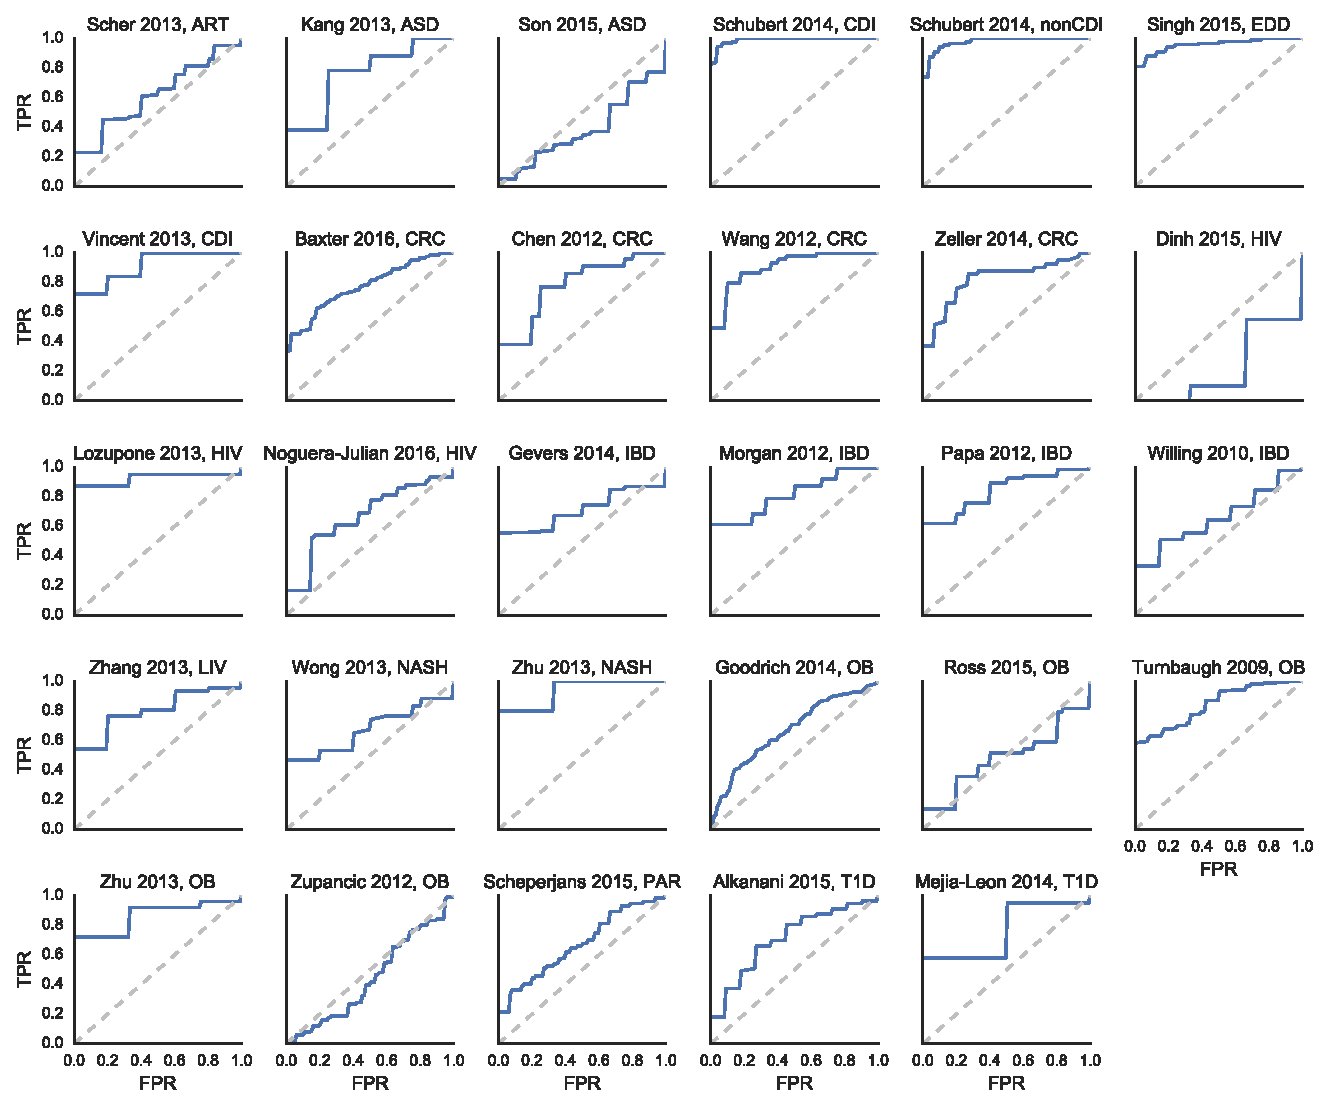
\includegraphics[width=\textwidth]{roc_curves.pdf}}
        \caption{ROC curves for each of the classifiers in Figure 1. Datasets are ordered alphabetically by disease and within disease by first author. FPR = false positive rate, TPR = true positive rate. ART = arthritis, ASD = autism spectrum disorder, CDI = \textit{Clostridium difficile} infection, CRC = colorectal cancer, EDD = enteric diarrheal disease, HIV = human immunodeficient virus, IBD = inflammatory bowel disease, LIV = liver disease, NASH = non-alcoholic steatohepatitis, nonCDI = non-\textit{Clostridium difficile} infection, OB = obesity, PAR = Parkinson's disease, T1D = type I diabetes.
}
        \label{fig:roc_curves}
        \end{center}
\end{figure}

%\newgeometry{textwidth=12in, left=1.5in}
%\newpage \pdfpagewidth=16in \pdfpageheight=18in

\begin{figure}[h]
	\begin{centering}
%	\makebox[\textwidth][c]{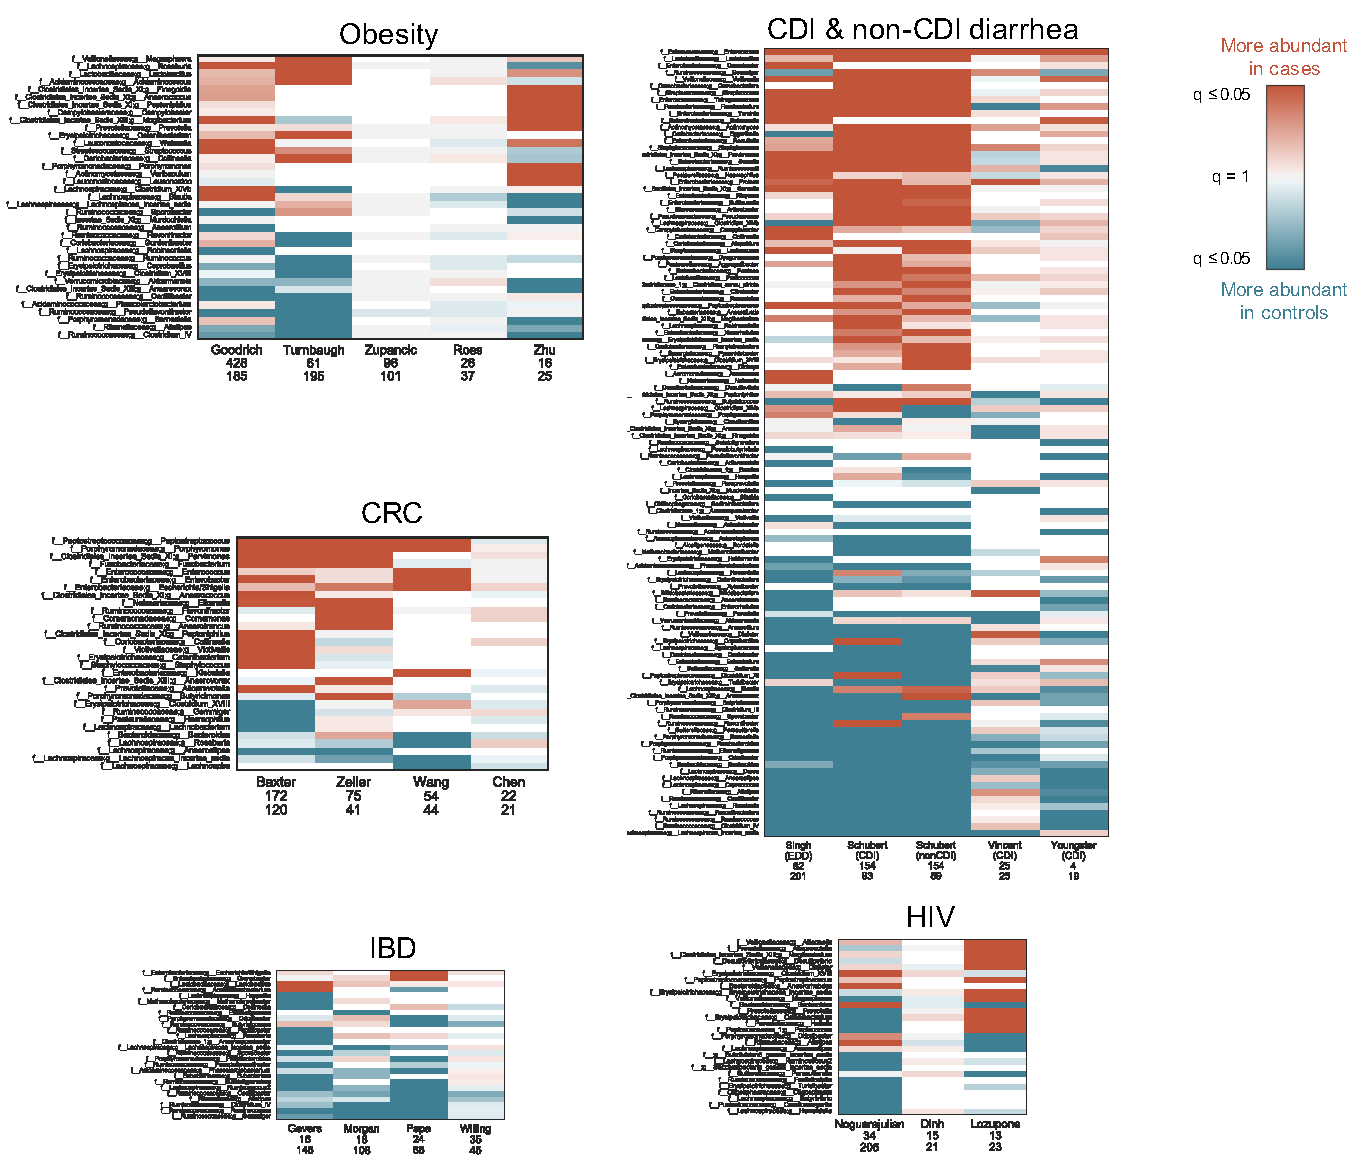
\includegraphics[width=\textwidth]{disease_specific_heatmaps_with_labels.pdf}}%
	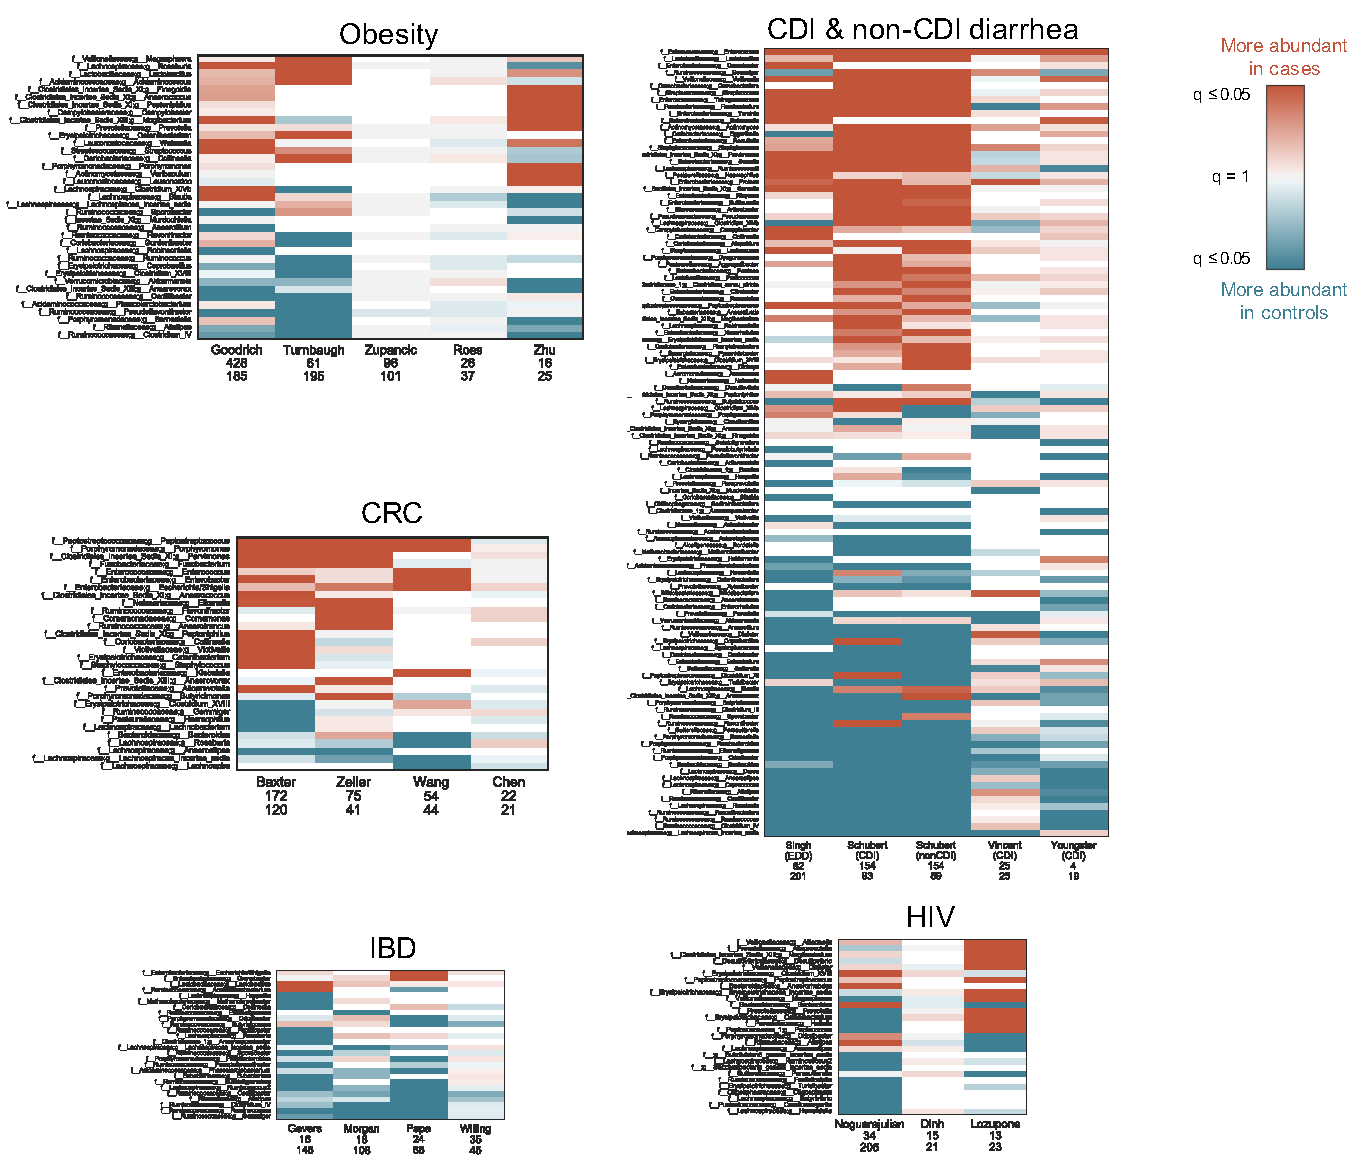
\includegraphics[width=\textwidth]{disease_specific_heatmaps_with_labels.pdf}
	\caption{Same heatmaps as in Figure 2, with rows labeled by family and genus taxonomy. Heatmaps show log10(q-values) for each disease (Kruskal-Wallis (KW) test, Benjamini-Hochberg FDR correction). Rows include all genera which were significant in at least one dataset within each disease, columns are datasets. Q-values are colored by direction of the effect, where red indicates higher mean abundance in disease patients and blue indicates higher mean abundance in controls. Opacity ranges from q = 0.05 to 1, where q values less than 0.05 are the most opaque and q values close to 1 are gray. White indicates that the genus was not present in that dataset. Within each heatmap, rows are ordered from most disease-associated (top) to most health-associated (bottom) (i.e. by the sum across rows of the log10(q-values), signed according to directionality of the effect).
}
	\label{fig:supp_dis_specific}
	\end{centering}
\end{figure}


%\restoregeometry
\FloatBarrier

% Core bugs with genus labels
%\newpage \pdfpagewidth=8.5in \pdfpageheight=27in
\FloatBarrier

\begin{figure}[h]
	\begin{center}
	\makebox[\textwidth][c]{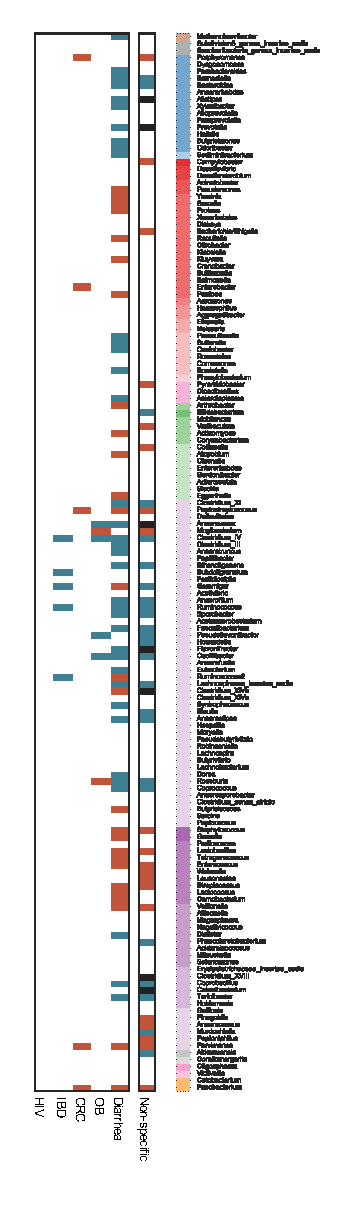
\includegraphics[width=0.37\textwidth]{meta_analysis_with_labels.pdf}}
    \captionsetup{font=footnotesize,labelfont=footnotesize}
	\caption{Panel A from Figure 3, with genus labels. Non-specific and disease-associated genera. Genera are in rows, arranged phylogenetically according to a PhyloT tree built from genus-level NCBI IDs (\url{http://phylot.biobyte.de}). Non-specific genera are associated with health (or disease) in at least two different \textit{diseases} (q $<$ 0.05, Kruskal-Wallis (KW) test, Benjamini-Hochberg FDR correction). Disease-specific genera are significant in the same direction in at least two \textit{studies} of the same disease (q $<$ 0.05, FDR KW test). As in Figure 2, blue indicates higher mean abundance in controls and red indicates higher mean abundance in patients. Black bars indicate mixed genera which were associated with health in two diseases and also associated with disease in two diseases. Disease-specific genera are shown for diseases with at least 3 studies.
}
	\label{fig:supp_meta_heatmap}
	\end{center}
\end{figure}

% Sample size, AUC, n sig, and balance for split cases analyses
\FloatBarrier
%\newpage \pdfpagewidth=8.5in \pdfpageheight=10in

\begin{figure}[h]
	\begin{center}
	\makebox[\textwidth][c]{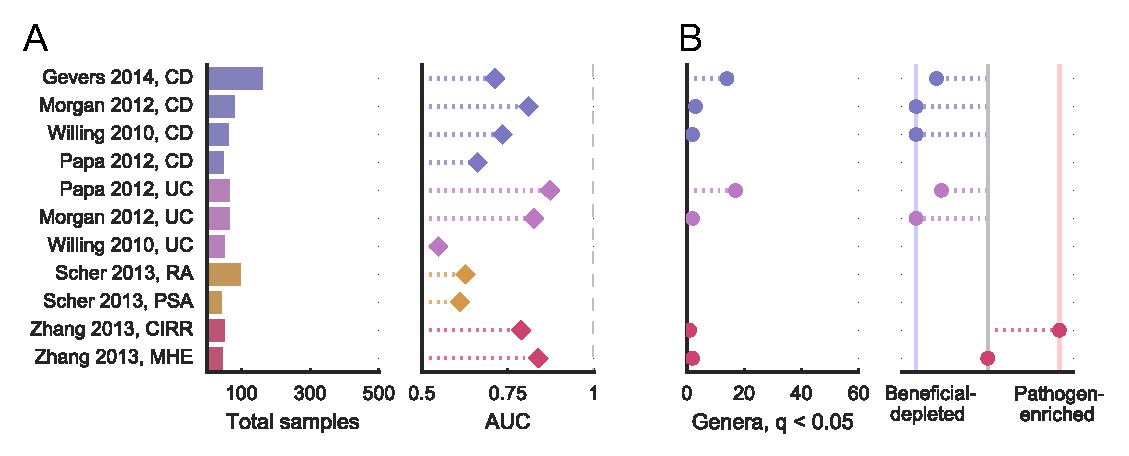
\includegraphics[width=\textwidth]{samplesize_auc_nsig_balance_split_cases.pdf}}%
	\caption{Same analysis as in Figure 1 for stratified patient groups. (A) Left: Total sample size for each comparison. Right: Area under the ROC curve (AUC) for genus-level random forest classifiers. (B) Left: Number of genera with q $<$ 0.05 (Kruskal-Wallis (KW) test, Benjamini-Hochberg FDR correction) for each type of patient group comparison. Right: Direction of microbiome shift,i.e. the percent of total associated genera which were enriched in diseased patients. In comparisons on the leftmost blue line, 100\% of associated (q $<$ 0.05, FDR KW test) genera are health-associated (i.e. depleted in patients relative to controls). In comparisons on the rightmost red line, 100\% of associated (q $<$ 0.05, FDR KW test) genera are disease-associated (i.e. enriched in patients relative to controls).
}
	\label{fig:split_cases_fig1}
	\end{center}
\end{figure}

% CD and UC qvalues heatmaps
\newpage
\begin{figure}[h]
	\begin{center}
	\makebox[\textwidth][c]{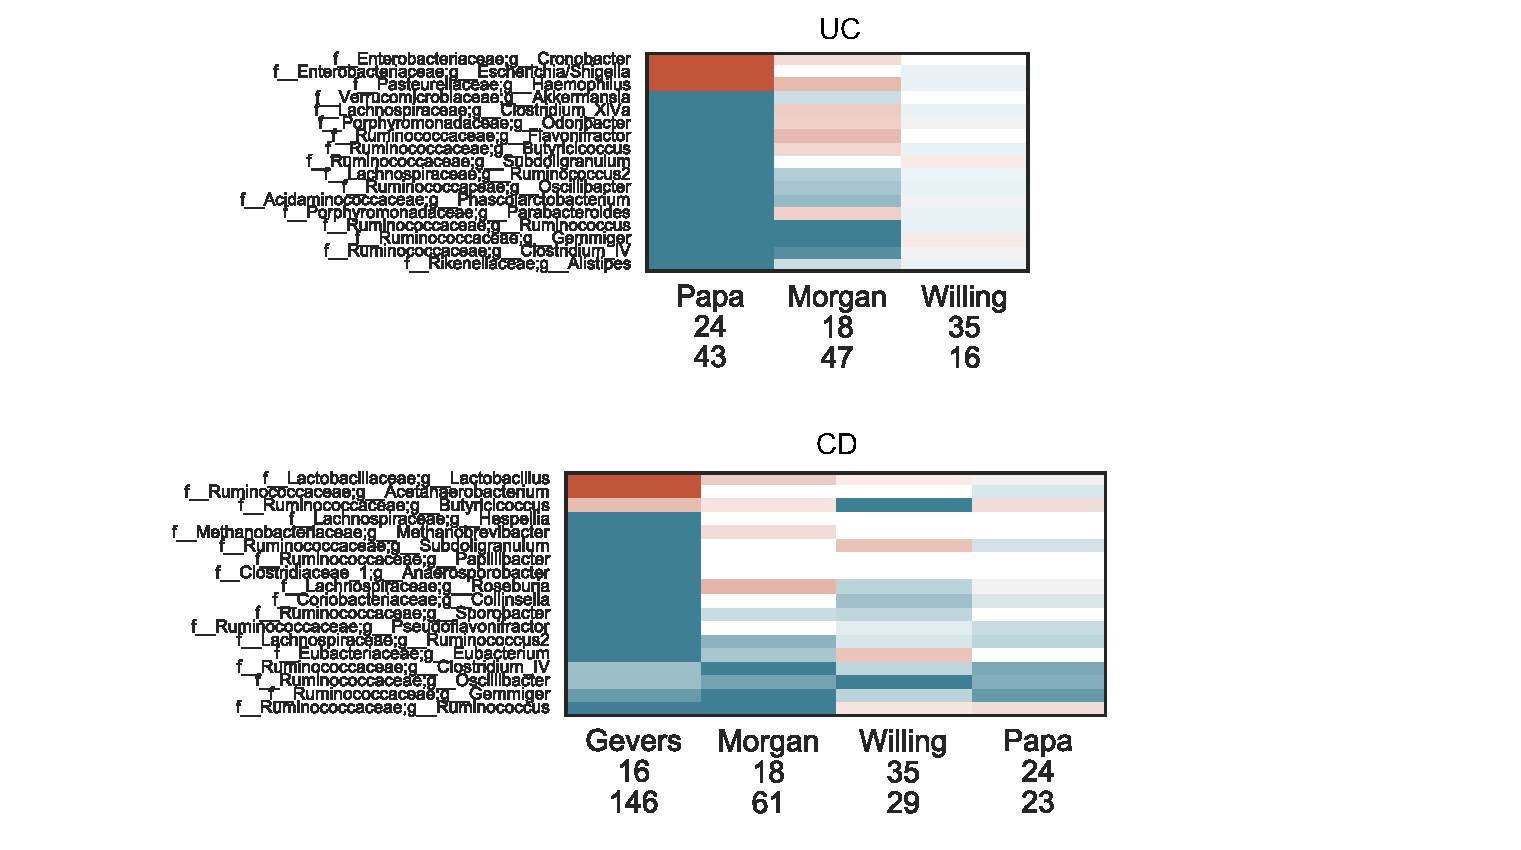
\includegraphics[width=1.1\textwidth]{disease_specific_heatmaps_with_labels_split_cases.pdf}}%
	\caption{Same results as presented in Figure 2 for ulcerative colitis (UC) and Crohn's disease (CD) IBD patients separately. Heatmaps show log10(q-values) for each comparison, with studies in columns and genera in rows (Kruskal-Wallis (KW) test, Benjamini-Hochberg FDR correction). Q-values are colored by direction of the effect, where red indicates higher mean abundance in disease patients and blue indicates higher mean abundance in controls. Opacity ranges from q = 0.05 to 1, where q values less than 0.05 are the most opaque and q values close to 1 are gray. White indicates that the genus was not present in that dataset. Within each heatmap, rows are ordered from most disease-associated (top) to most health-associated (bottom) (i.e. by the sum across rows of the log10(q-values), signed according to directionality of the effect).
}
	\label{fig:split_cases_heatmaps}
	\end{center}
\end{figure}

% Shannon alpha diversity
\newpage
\begin{figure}[h]
	\begin{center}
	\makebox[\textwidth][c]{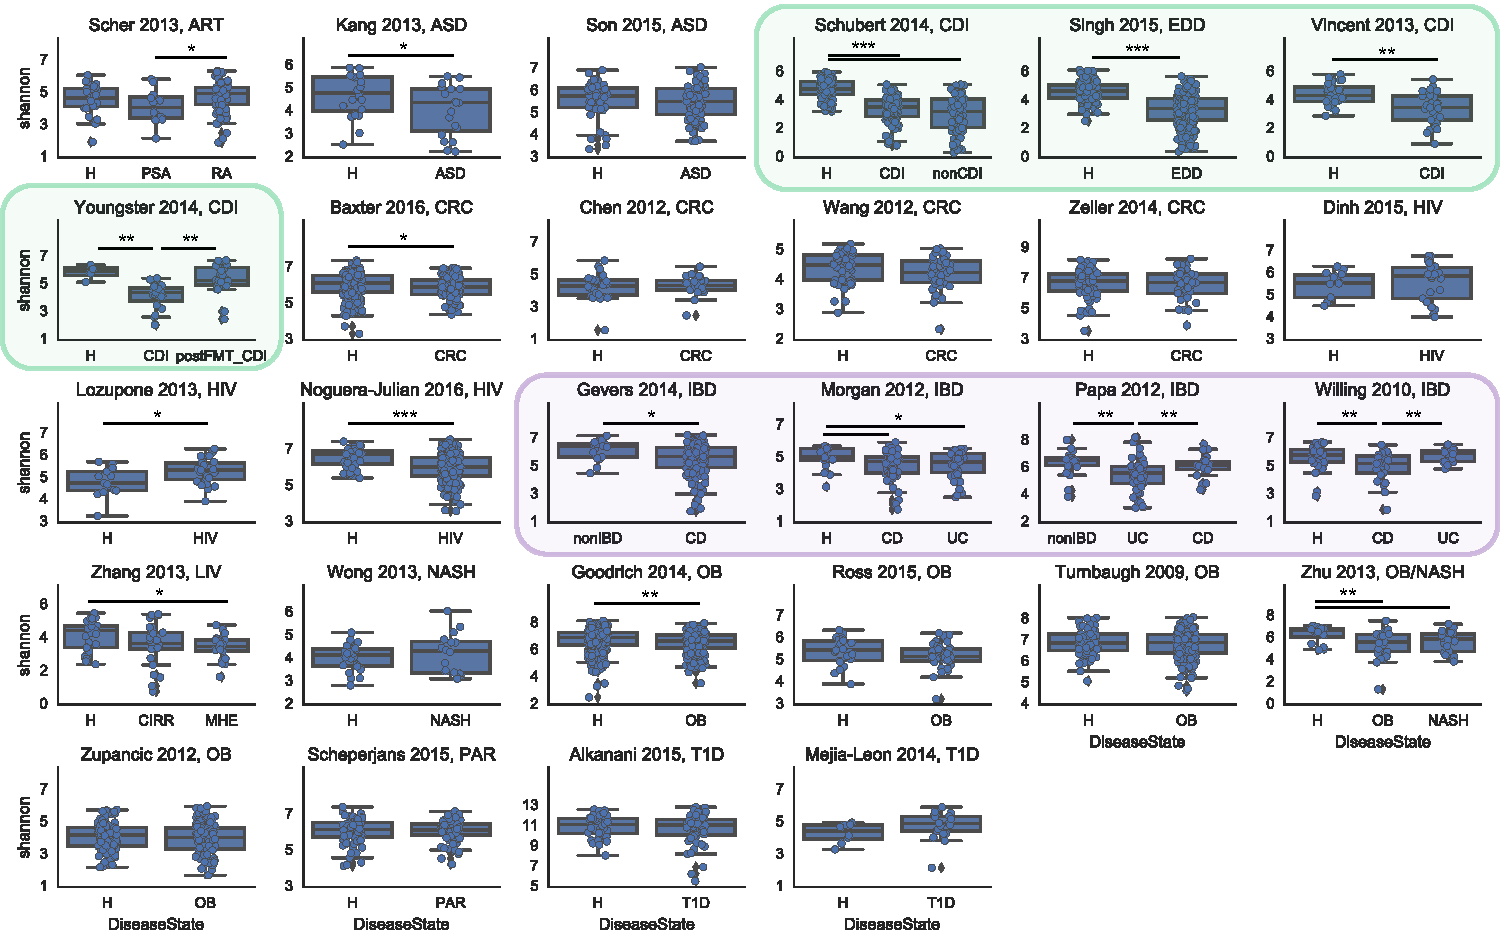
\includegraphics[width=\textwidth]{alpha_diversity_shannon.pdf}}
    \captionsetup{font=footnotesize,labelfont=footnotesize}
	\caption{Reduction in alpha diversity is not a reliable indicator of ``dysbiosis.'' Shannon alpha diversity index across all patient groups in all studies, calculated on OTUs (i.e. not collapsed to genus level, and including unannotated OTUs). Diarrheal patients consistently have lower alpha diversity than non-diarrheal controls (green box). Crohn's disease (CD) patients also show a slight reduction of alpha diversity relative to controls in three out of four IBD studies and ulcerative colitis (UC) patients in two studies (purple box). Obese patients have inconsistent and small reductions in alpha diversity, consistent with a previous meta-analysis \cite{Sze07092016}. $\ast: 0.01 < p < 0.05, \ast\ast: 10^{-4} < p < 0.01, \ast\ast\ast: p < 10^{-4}$. P values are calculated from a two-sided T-test (using \texttt{scipy.stats.ttest\_ind}) and are not corrected for multiple tests. Note that the datasets with multiple case groups (Zhu et al. (OB/NASH, 2013) and Schubert et al. (CDI/non-CDI, 2014)) are presented only once in this plot. ART = arthritis, ASD = austism spectrum disorder, CD = Crohn's disease, CDI = \textit{Clostridium difficile} infection, CIRR = liver cirrhosis, CRC = colorectal cancer, EDD = enteric diarrheal disease, H = healthy, HIV = human immunodeficiency virus, LIV = liver diseases,  MHE =  minimal hepatic encephalopathy, NASH = non-alcoholic steatohepatitis, OB = obesity, PAR = Parkinson's disease, PSA = psoriatic arthritis, RA = rheumatoid arthritis, T1D = type I diabetes, UC = ulcerative colitis. nonCDI controls are patients with diarrhea who tested negative for \textit{C. difficile} infection. nonIBD controls are patients  with gastrointestinal symptoms but no intestinal inflammation.
}
	\label{fig:fig_alpha}
	\end{center}
\end{figure}

% Chao1 alpha diversity
\newpage
\begin{figure}[h]
	\begin{center}
	\makebox[\textwidth][c]{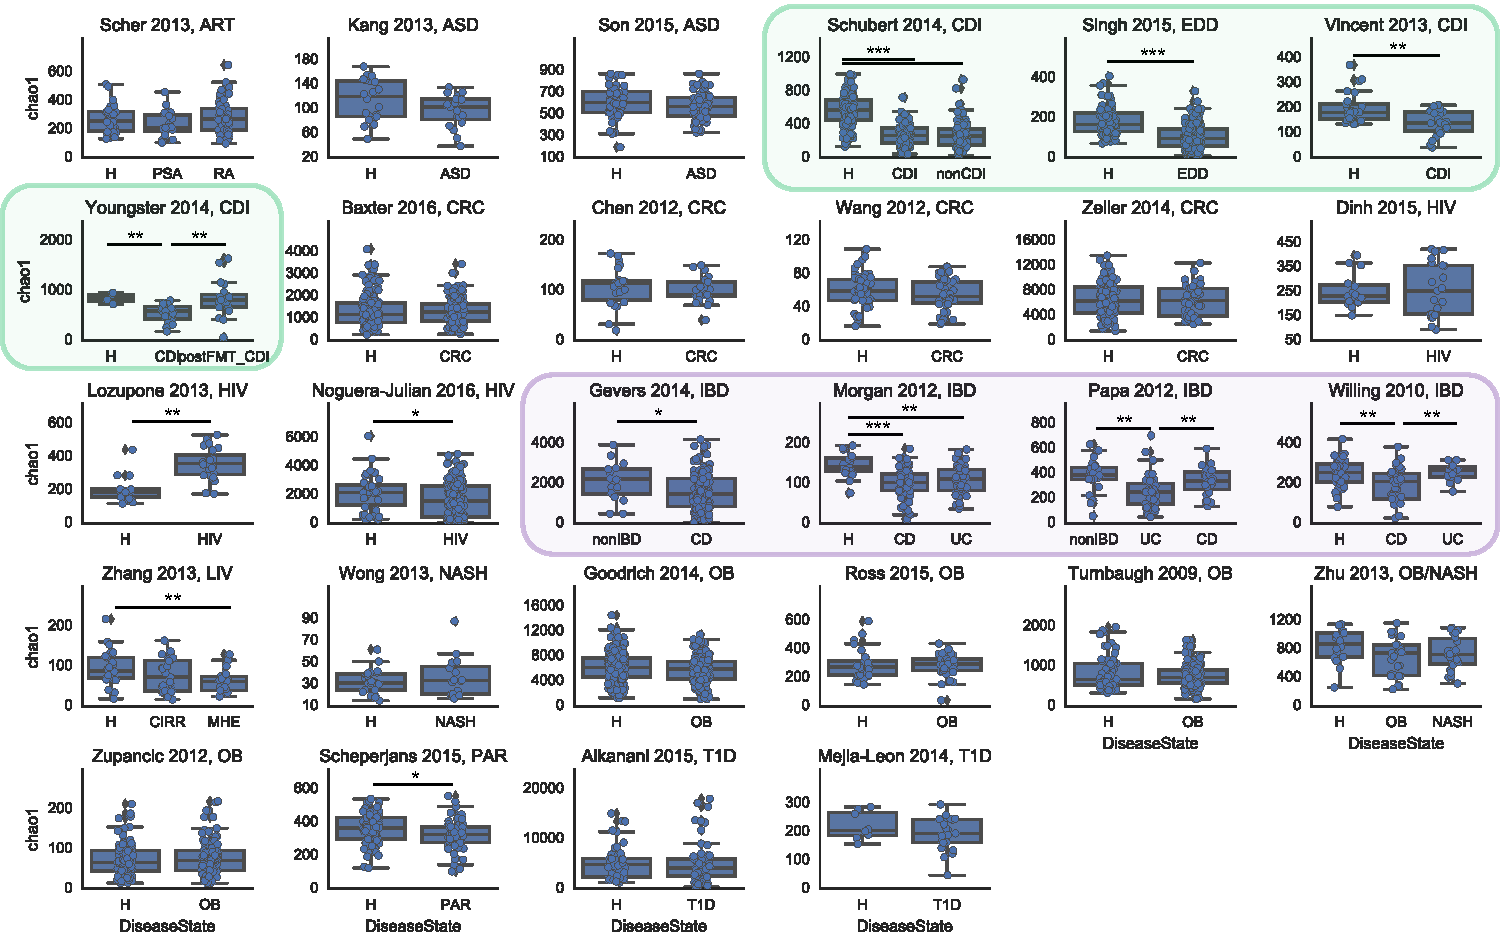
\includegraphics[width=1\textwidth]{alpha_diversity_chao1.pdf}}
    \captionsetup{font=footnotesize,labelfont=footnotesize}
	\caption{Chao1 alpha diversity across all patient groups in all studies, calculated on OTUs (i.e. not collapsed to genus level, and including unannotated OTUs). $\ast: 0.01 < p < 0.05, \ast\ast: 10^{-4} < p < 0.01, \ast\ast\ast: p < 10^{-4}$. P values are calculated from a two-sided T-test (using \texttt{scipy.stats.ttest\_ind}) and are not corrected for multiple tests. Note that the datasets with multiple case groups (Zhu et al. (OB/NASH, 2013) and Schubert et al. (CDI/non-CDI, 2014)) are presented only once in this plot. ART = arthritis, ASD = austism spectrum disorder, CD = Crohn's disease, CDI = \textit{Clostridium difficile} infection, CIRR = liver cirrhosis, CRC = colorectal cancer, EDD = enteric diarrheal disease, H = healthy, HIV = human immunodeficiency virus, LIV = liver diseases,  MHE =  minimal hepatic encephalopathy, NASH = non-alcoholic steatohepatitis, OB = obesity, PAR = Parkinson's disease, PSA = psoriatic arthritis, RA = rheumatoid arthritis, T1D = type I diabetes, UC = ulcerative colitis. nonCDI controls are patients with diarrhea who tested negative for \textit{C. difficile} infection. nonIBD controls are patients  with gastrointestinal symptoms but no intestinal inflammation.
}
	\label{fig:fig_alpha_chao1}
	\end{center}
\end{figure}

% Simpson alpha diversity
\newpage
\begin{figure}[h]
	\begin{center}
	\makebox[\textwidth][c]{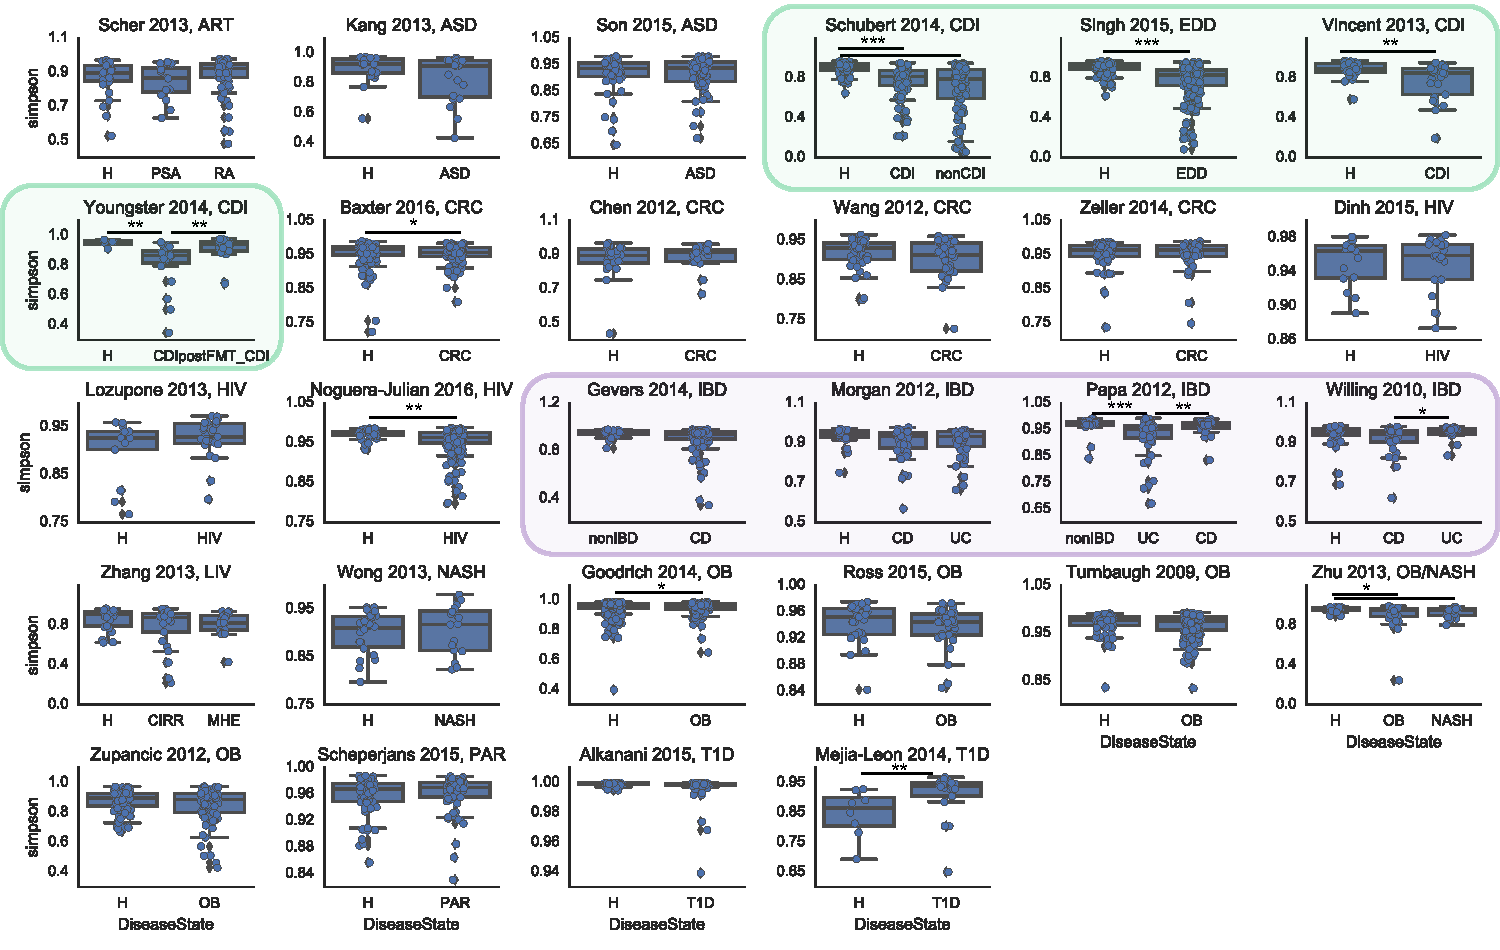
\includegraphics[width=\textwidth]{alpha_diversity_simpson.pdf}}
    \captionsetup{font=footnotesize,labelfont=footnotesize}
	\caption{Simpson alpha diversity across all patient groups in all studies, calculated on OTUs (i.e. not collapsed to genus level, and including unannotated OTUs). $\ast: 0.01 < p < 0.05, \ast\ast: 10^{-4} < p < 0.01, \ast\ast\ast: p < 10^{-4}$. P values are calculated from a two-sided T-test (using \texttt{scipy.stats.ttest\_ind}) and are not corrected for multiple tests. Note that the datasets with multiple case groups (Zhu et al. (OB/NASH, 2013) and Schubert et al. (CDI/non-CDI, 2014)) are presented only once in this plot. ART = arthritis, ASD = austism spectrum disorder, CD = Crohn's disease, CDI = \textit{Clostridium difficile} infection, CIRR = liver cirrhosis, CRC = colorectal cancer, EDD = enteric diarrheal disease, H = healthy, HIV = human immunodeficiency virus, LIV = liver diseases,  MHE =  minimal hepatic encephalopathy, NASH = non-alcoholic steatohepatitis, OB = obesity, PAR = Parkinson's disease, PSA = psoriatic arthritis, RA = rheumatoid arthritis, T1D = type I diabetes, UC = ulcerative colitis. nonCDI controls are patients with diarrhea who tested negative for \textit{C. difficile} infection. nonIBD controls are patients  with gastrointestinal symptoms but no intestinal inflammation.
}
	\label{fig:fig_alpha_simpson}
	\end{center}
\end{figure}

% Healthy vs. disease classifier
\newpage
\begin{figure}[h]
	\begin{center}
	\makebox[\textwidth][c]{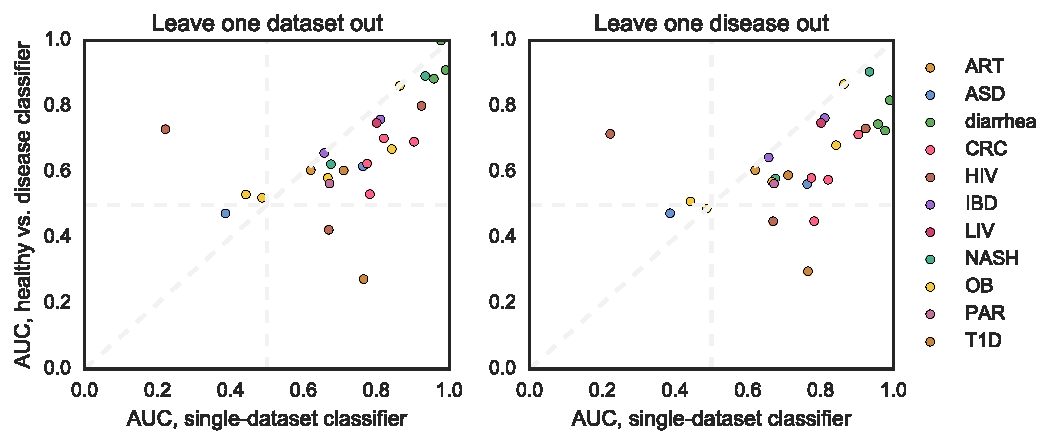
\includegraphics[width=1\textwidth]{healthy_vs_disease_classifier.pdf}}%
	\caption{\textit{Both x-axes}: the area under the ROC curve (AUC) from each dataset's single classifier. Left: leave-one-dataset-out classifier. \textit{y-axis}: the AUC of a classifier trained on all other datasets to distinguish healthy from unhealthy patients, tested on the left out dataset. Right: leave-one-disease-out classifier. \textit{y-axis}: AUC from a classifier trained to distinguish healthy from unhealthy patients on all datasets except those of the tested disease. AUCs for each dataset were built from the classification probabilities on each test sample.
}
	\label{fig:overall_classifier}
	\end{center}
\end{figure}

% Different ways to define core response
\FloatBarrier
%\newpage \pdfpagewidth=8.5in \pdfpageheight=15in

\begin{figure}[h]
	\begin{center}
	\makebox[\textwidth][c]{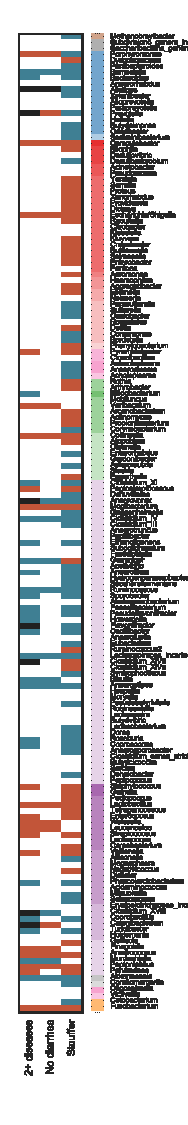
\includegraphics[width=0.22\textwidth]{different_core_defns.pdf}}
    \captionsetup{font=footnotesize,labelfont=footnotesize}
	\caption{The majority of non-specific microbes are robust to the exclusion of diarrhea datasets from consideration. The right-most bar shows order-level phylogeny, colored as in Figure 3A of the main paper. The left bar of the heatmap shows the original non-specific microbes, including all datasets. The middle bar shows the re-defined non-specific responders after excluding all diarrhea datasets. The right bar of the heatmap shows the non-specific microbes defined using Stouffer’s method, combining one-tailed q-values across datasets and weighting by the square root of sample size (Stouffer combined q $<$ 0.05).
}
	\label{fig:core_defns}
	\end{center}
\end{figure}


% Significance of shared response
\FloatBarrier
%\newpage \pdfpagewidth=8.5in \pdfpageheight=11in

\begin{figure}[h]
	\begin{center}
	\makebox[\textwidth][c]{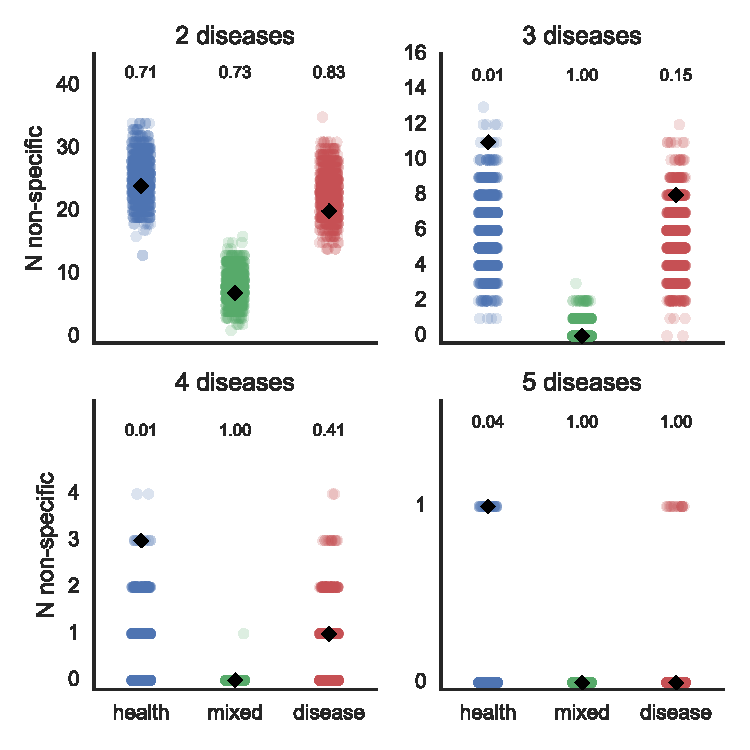
\includegraphics[width=\textwidth]{core_significance.pdf}}%
	\caption{Empirical null distribution of the number of non-specific responders (colored points, x-axis indicates directionality of response), overlayed with the actual observed number of non-specific responders (black diamonds) for different defining heuristics (axis titles, i.e. ``3 diseases`` means that a genus needed to be significant (q $<$ 0.05, Kruskal-Wallis (KW) test, Benjamini-Hochberg FDR correction) in three diseases in the same direction to be considered a non-specific responder). Empirical one-tailed p-values are printed above each distribution.
}
	\label{fig:core_sig}
	\end{center}
\end{figure}

% RF param search - gini criteria
\newpage
\begin{landscape}
\begin{figure}[h]
	\begin{center}
	\makebox[\textwidth][c]{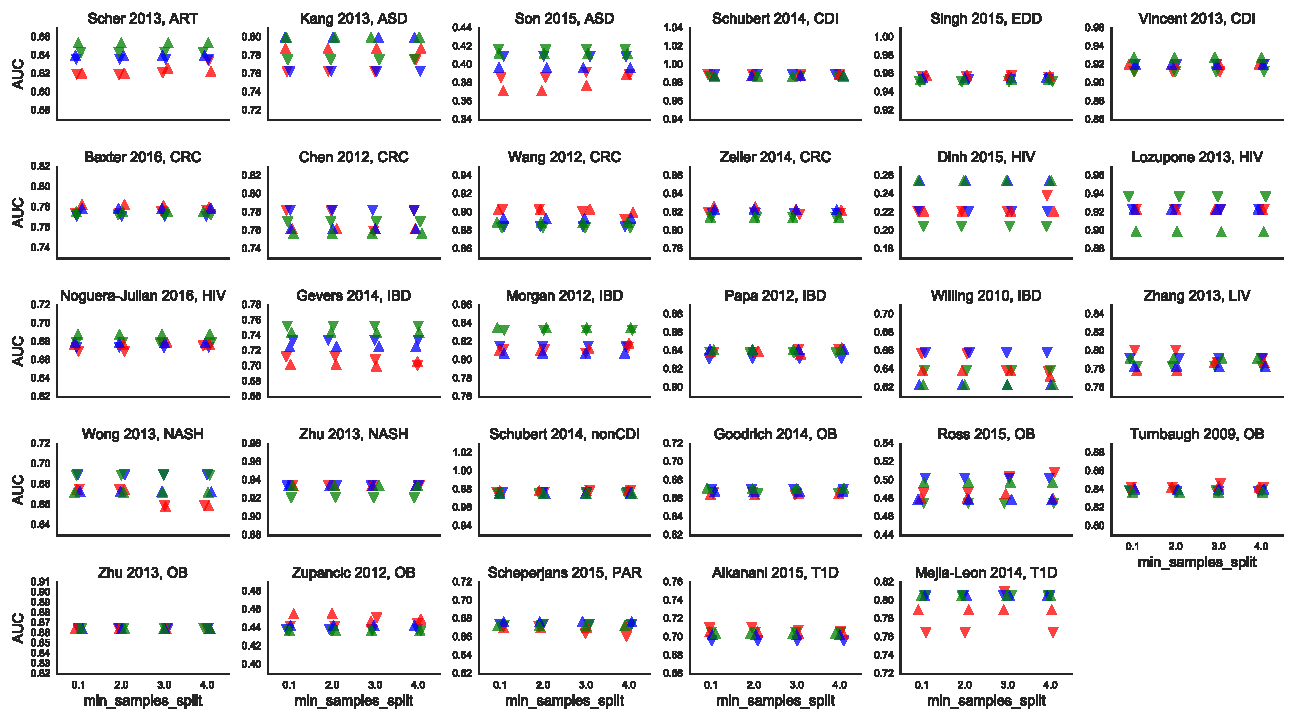
\includegraphics[width=1.4\textwidth]{rf_params_gini.pdf}}%
	\caption{Varying Random Forest parameters does not significantly affect area under the ROC curve in classifying cases from controls (Gini criteria). Random Forest classifiers built by using the Gini impurity (``gini'') split criteria (``scikit-learn RandomForestClassifier''). Upward-pointing triangles are classifiers built with 10000 estimators; downward-pointing triangles are built with 1000 estimators. Colors indicate the value of \texttt{min\_samples\_leaf} (the minimum number of samples required to be at a leaf node): red = 1, blue = 2, green = 3. X-axes are the value of \texttt{min\_samples\_split} (the minimum number of samples required to split an internal node) \cite{scikit-learn}. All Random Forests were built using the random state seed $12345$.
}
	\label{fig:rf_params_gini}
	\end{center}
\end{figure}

% RF param search - entropy criteria
\newpage
\begin{figure}[h]
	\begin{center}
	\makebox[\textwidth][c]{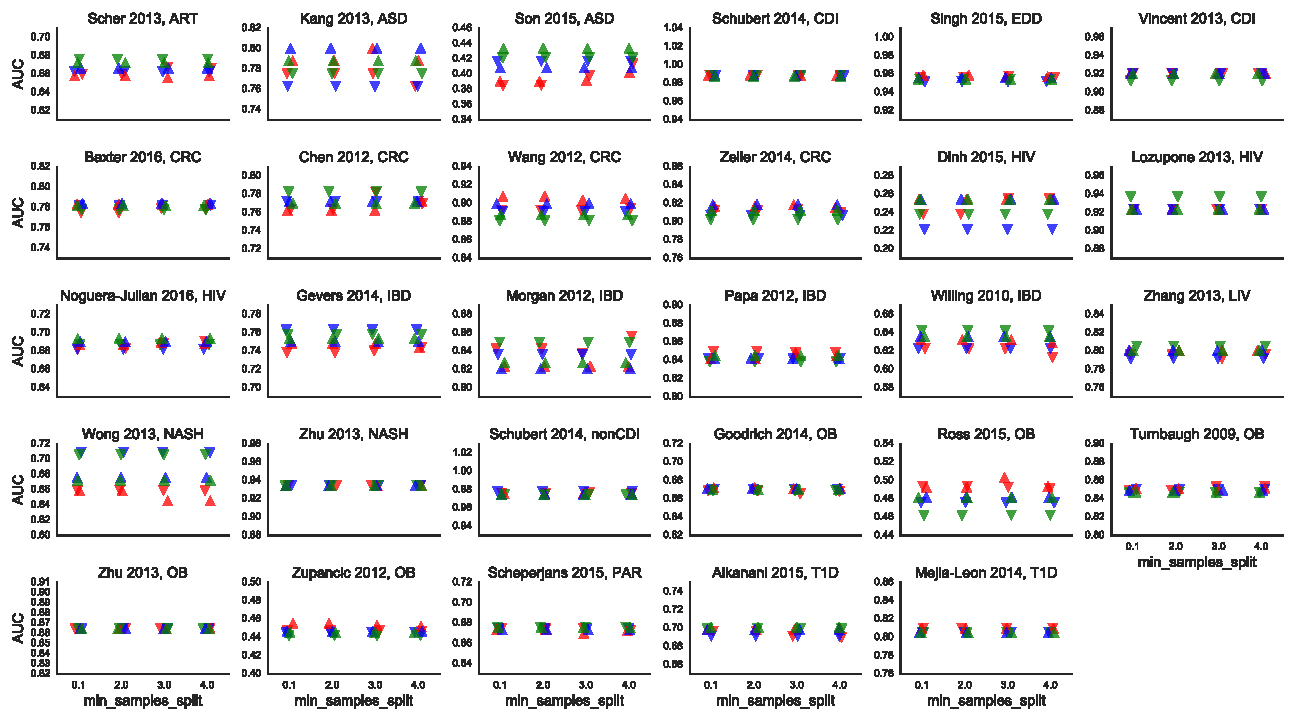
\includegraphics[width=1.4\textwidth]{rf_params_entropy.pdf}}%
	\caption{Varying Random Forest parameters does not significantly affect area under the ROC curve in classifying cases from controls (entropy criteria). Random Forest classifiers built by using the entropy (``entropy'') split criteria (``scikit-learn RandomForestClassifier''). Upward-pointing triangles are classifiers built with 10000 estimators; downward-pointing triangles are built with 1000 estimators. Colors indicate the value of \texttt{min\_samples\_leaf} (the minimum number of samples required to be at a leaf node): red = 1, blue = 2, green = 3. X-axes are the value of \texttt{min\_samples\_split} (the minimum number of samples required to split an internal node) \cite{scikit-learn}. All Random Forests were built using the random state seed $12345$.
}
	\label{fig:rf_params_entropy}
	\end{center}
\end{figure}
\end{landscape}

% Heatmap with results for all datasets (all sig genera) - qvalues
\FloatBarrier
%\newgeometry{textwidth=18in, left=1.5in}
%\newpage \pdfpagewidth=28in \pdfpageheight=28in

\begin{figure}[h]
	\begin{center}
	\makebox[\textwidth][c]{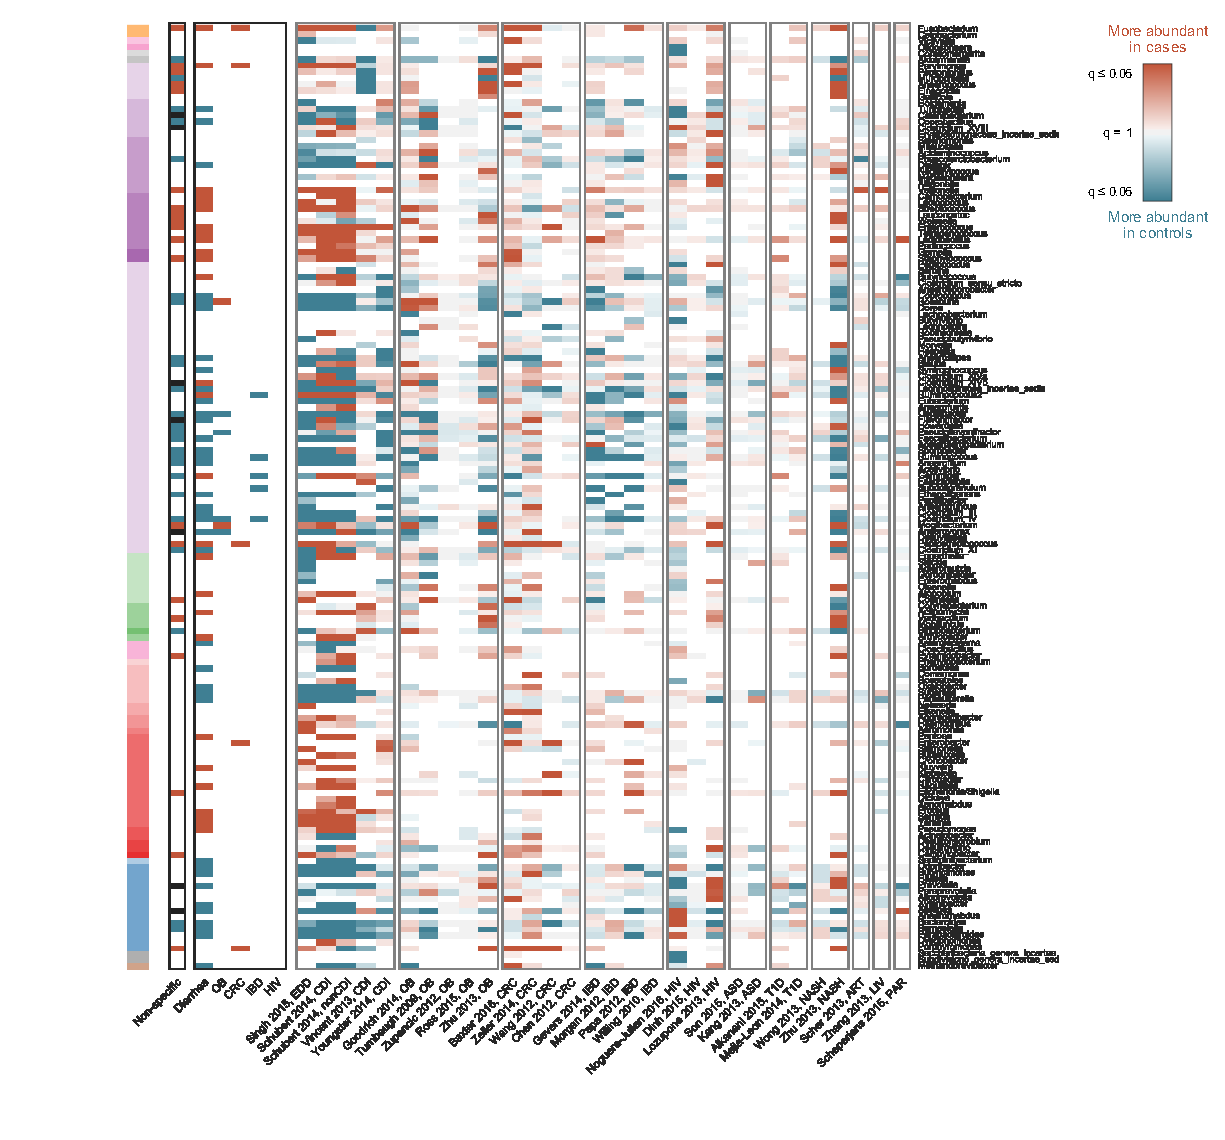
\includegraphics[width=1.2\textwidth]{overall_heatmap_log10qvalues.pdf}}
	%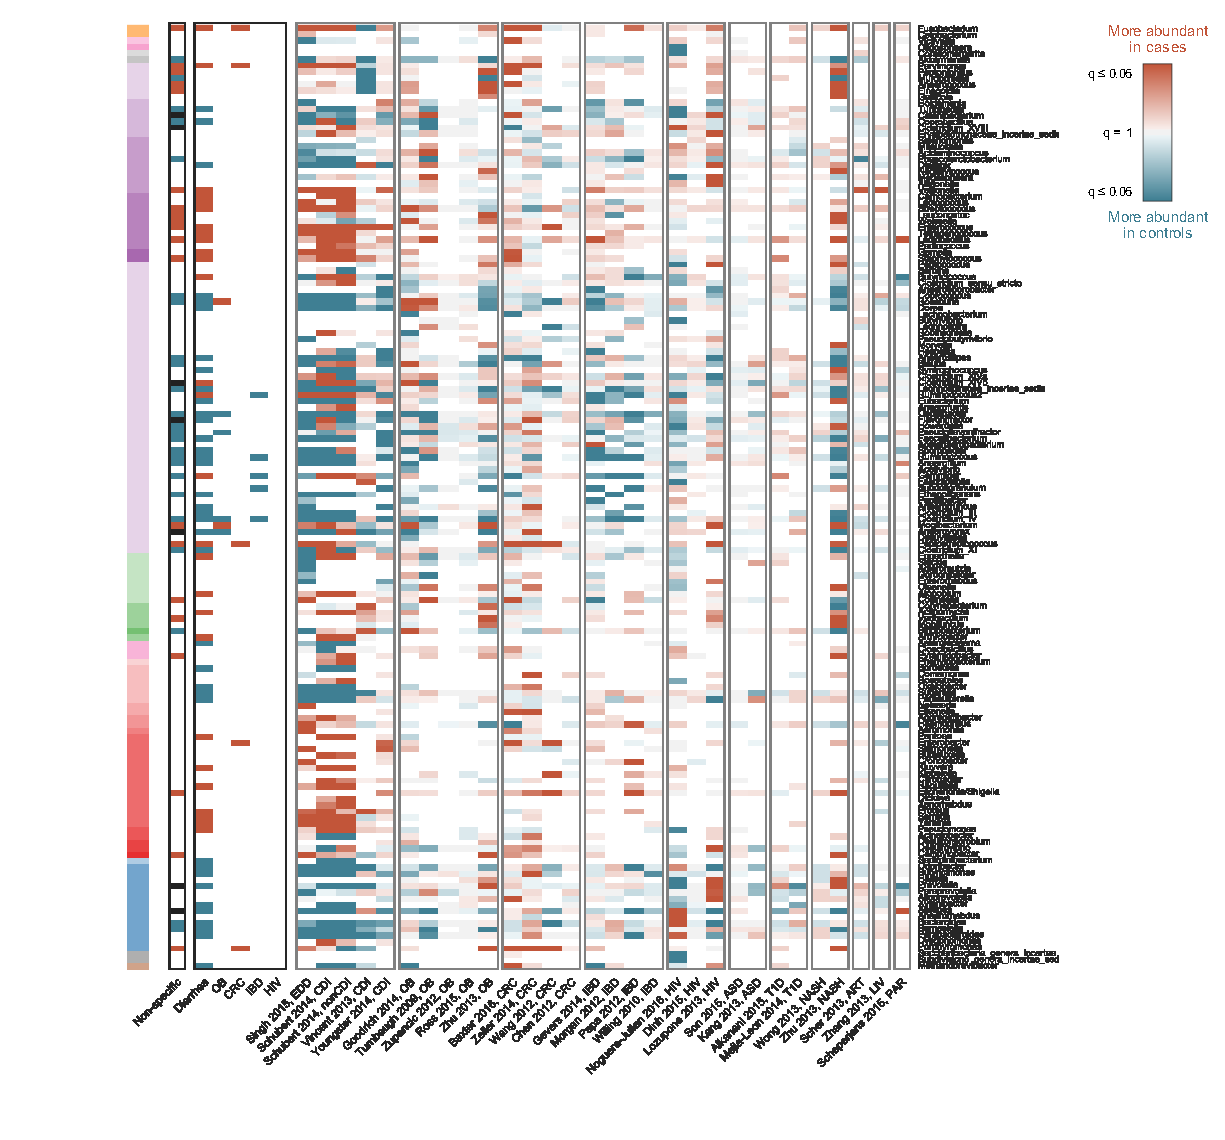
\includegraphics[width=1.2\textwidth]{overall_heatmap_log10qvalues.pdf}
    \captionsetup{font=footnotesize,labelfont=footnotesize}
	\caption{Heatmap of log10(q values) for all genera which were significant (q $<$ 0.05, Kruskal-Wallis (KW) test, Benjamini-Hochberg FDR correction) in at least one dataset, across all studies. Rows are genera, ordered phylogenetically (as in Figure 3A). Columns are datasets, grouped by disease and ordered according to total sample size (decreasing from left to right). The first and second heatmap panels from the left are the same as in Figure 3A. Q-values are colored according to directionality of the effect, where red indicates higher mean abundance in patients relative to controls and blue indicates higher mean abundance in controls. Opacity indicates significance and ranges from 0.05 to 1, where q-values less than 0.05 are the darkest colors and q-values close to 1 are gray. White indicates that the genus was not present in that dataset. ART = arthritis, ASD = autism spectrum disorder, CDI = \textit{Clostridium difficile} infection, CRC = colorectal cancer, EDD = enteric diarrheal disease, HIV = human immunodeficient virus, IBD = inflammatory bowel disease, LIV = liver disease, NASH = non-alcoholic steatohepatitis, nonCDI = non-\textit{Clostridium difficile} infection, OB = obesity, PAR = Parkinson's disease, T1D = type I diabetes.
}
	\label{fig:overall_heatmap_qvalues}
	\end{center}
\end{figure}

% Heatmap with results for all datasets (all sig genera) - effect size
\newpage
\begin{figure}[h]
	\begin{center}
	\makebox[\textwidth][c]{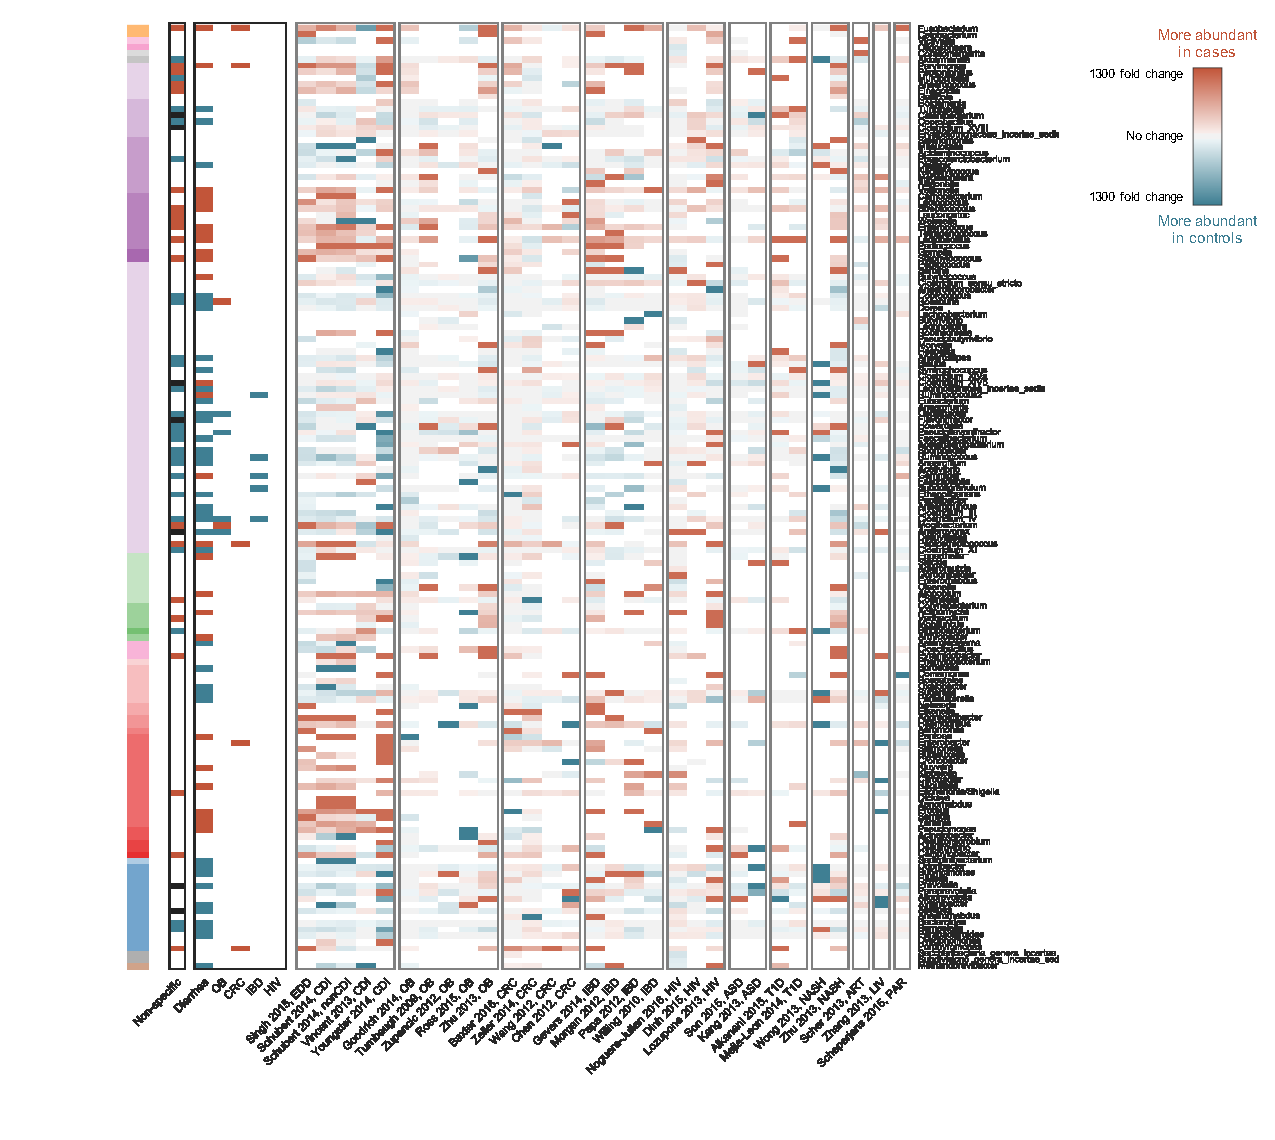
\includegraphics[width=1.2\textwidth]{overall_heatmap_log2change.pdf}}
	%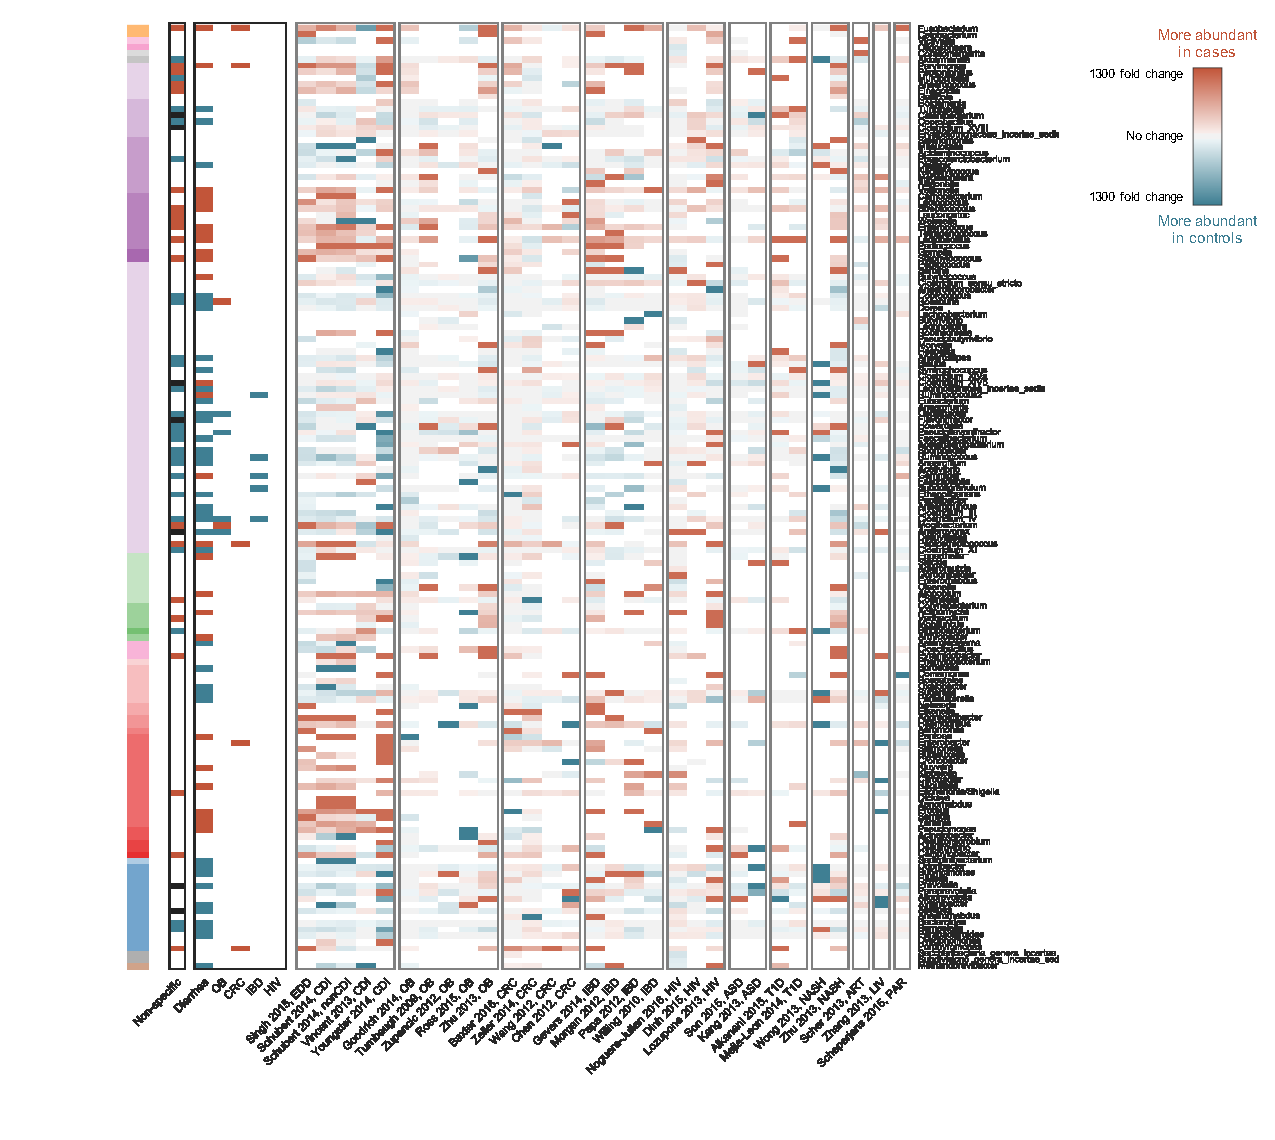
\includegraphics[width=24in]{overall_heatmap_log2change.pdf}
    \captionsetup{font=footnotesize,labelfont=footnotesize}
	\caption{Heatmap of log-fold change between cases and controls (i.e. $log_2(\frac{\text{mean abundance in cases}}{\text{mean abundance in controls}}$) for all genera which were significant (q $<$ 0.05) in at least one dataset, across all studies. Rows are genera, ordered phylogenetically (as in Figure 3A). Columns are datasets, grouped by disease and ordered according to total sample size (decreasing from left to right). The first and second heatmap panels from the left are the same as in Figure 3A. Values are colored according to directionality of the effect, where red indicates higher mean abundance in patients relative to controls and blue indicates higher mean abundance in controls. Opacity indicates fold change and ranges from 1300 to 0, where fold changes greater than 1300 are the darkest colors and fold changes close to 0 are gray. White indicates that the genus was not present in that dataset. ART = arthritis, ASD = autism spectrum disorder, CDI = \textit{Clostridium difficile} infection, CRC = colorectal cancer, EDD = enteric diarrheal disease, HIV = human immunodeficient virus, IBD = inflammatory bowel disease, LIV = liver disease, NASH = non-alcoholic steatohepatitis, nonCDI = non-\textit{Clostridium difficile} infection, OB = obesity, PAR = Parkinson's disease, T1D = type I diabetes.
}
	\label{fig:overall_heatmap_foldchange}
	\end{center}
\end{figure}

\begin{singlespace}
\bibliographystyle{unsrt}
\bibliography{meta-analysis/refs}
\end{singlespace}



% Include the biblio file if you want to have a single, monolithic list of references
% at the end of the thesis. If you do not include the biblio file, you'll have to put
% bibliographies at the end of each chapter.
%\include{biblio}

\end{document}
